\documentclass{beamer}

% PERGUNTAR PARA GONZALO
% - cronogroma?
% - falo da publicação em andamento?

% TODO
% - separar em colunas o sumário
% - mostrar sempre o sumário em inícios de seção
% - pontos em finais de frases
% x número de páginas
% - retirar equações, deixar descrições ao lado da figura de dialética/opos/inov
% - colocar essas medidas no seu devido lugar
% - melhorar tamanho de tabelas
% - adicionar imagens em miniatura depois de Artistas Escolhidos
% - no Período Barroco (e Moderno) mostrar imagens para cada item
% - adicionar imagens ilustrando cada passo de proc de imagem
% - Segmentação: adicionar os métodos usados (Watershed, ...), parâmetros do slic
% - Atributos: dividir a tabela em cada classe de atributos
% - Resultados: período barroco e moderno, colocar "closes" da projeção ou histograma, mudando a cada tópico

% adicionar quando falar sobre os vários movimentos artísticos: http://www.wardshelley.com/paintings/dtbody/downtownbody.jpg
% http://blog.ibs-b.hu/wp-content/uploads/2012/10/history_of_art_timeline.jpg
% http://blog.ibs-b.hu/wp-content/uploads/2012/10/ArtTheoryMap20100905103543-llfocrmsjlrckoy.png

%
% Choose how your presentation looks.
%
% For more themes, color themes and font themes, see:
% http://deic.uab.es/~iblanes/beamer_gallery/index_by_theme.html
%
\mode<presentation>
{
  \usetheme{Frankfurt}      % or try Darmstadt, Madrid, Warsaw, ...
  \definecolor{ifsc}{rgb}{.43,.61,.78} % ifsc mais escuro
  \usecolortheme[named=ifsc]{structure} % or try albatross, beaver, crane, ...
  \usefonttheme{default}  % or try serif, structurebold, ...
  \setbeamertemplate{navigation symbols}{}
  \setbeamertemplate{caption}[numbered]

  \setbeamertemplate{note page}[compress]

  \setbeamertemplate{itemize items}[default]
  \setbeamertemplate{enumerate items}[default]

  \setbeamercolor{frametitle}{fg = black}
  \setbeamercovered{transparent}

%\titlegraphic{
\includegraphics{figs/ifsc_usp}}

% \defbeamertemplate*{title page}{customized}[1][]
% {\centering
%  \setbeamercolor{title}{bg=ifsc,fg=white}
%  \begin{beamercolorbox}[sep=5pt,center]{title}
%  \usebeamerfont{title}\inserttitle\par
%   \usebeamerfont{subtitle}\insertsubtitle
%   \end{beamercolorbox}
%    \par\medskip
%   \usebeamerfont{author}\insertauthor\par\medskip
%   \inserttitlegraphic \par\medskip
%   \usebeamerfont{institute}\insertinstitute\par\medskip
  
%   \usebeamerfont{date}\insertdate\par
% }

\defbeamertemplate*{title page}{customized}[1][]
{\centering
 \setbeamercolor{title}{bg=ifsc,fg=white}
 \begin{beamercolorbox}[sep=5pt,center]{title}
 \usebeamerfont{title}\inserttitle\par
  \end{beamercolorbox}
   \par\medskip\medskip\medskip
   \begin{columns}
   \begin{column}{0.2\textwidth}
   
\includegraphics[width=.8\columnwidth]{figs/ifsc_usp}
   \end{column}

   \begin{column}{0.6\textwidth}
   \centering{
  \usebeamerfont{author}\insertauthor\par\medskip\medskip
  %\inserttitlegraphic \par\medskip
  \usebeamerfont{institute}\insertinstitute\par\medskip\medskip
  
  \usebeamerfont{date}\insertdate\par
  }
  \end{column}
  \begin{column}{0.2\textwidth}
  
\includegraphics[width=\columnwidth]{figs/brasao_usp_pb}
  \end{column}
  \end{columns}
}

\setbeamertemplate{footline}
{%
  \begin{beamercolorbox}[colsep=1.5pt]{upper separation line foot}
  \end{beamercolorbox}
  \hbox{%
 \begin{beamercolorbox}[wd=0.7\paperwidth, ht=2.5ex, dp=1.125ex, left]{title in head/foot}%
      \usebeamerfont{title in head/foot}\hspace*{2ex}\insertshorttitle
    \end{beamercolorbox}%

    \begin{beamercolorbox}[wd=0.2\paperwidth, ht=2.5ex, dp=1.125ex, center]{title in head/foot}%
      \usebeamerfont{author in head/foot}{\insertshortinstitute }
    \end{beamercolorbox}%
   
    \begin{beamercolorbox}[wd=0.1\paperwidth, ht=2.5ex, dp=1.125ex, right]{title in head/foot}%
      \usebeamerfont{title in head/foot}\insertframenumber/\inserttotalframenumber\hspace*{2ex}
    \end{beamercolorbox}}
  \begin{beamercolorbox}[colsep=1.5pt]{lower separation line foot}
  \end{beamercolorbox}
}

} 

\usepackage[brazil]{babel}
\usepackage[utf8x]{inputenc}
\usepackage{multirow}
\usepackage{tikz}
\usepackage{setspace}

\tikzset{
    vertex/.style = {
        circle,
        fill            = black,
        outer sep = 2pt,
        inner sep = 1pt,
    }
}
%\usepackage[numberedbib]{apacite}
\usepackage{natbib} 
\usepackage{multicol}

\title[Um estudo quantitativo sobre a evolução de
movimentos artísticos
]{Um estudo quantitativo sobre a evolução de
movimentos artísticos}
\author{Vilson Vieira}
\institute[IFSC/USP]{Instituto de Física de São Carlos \\
Universidade de São Paulo \\
Departamento de Física e Ciência dos Materiais \\
Grupo de Computação Interdisciplinar
}
\date{\today}

\begin{document}

\begin{frame}
  \titlepage
\end{frame}

%% sumário 
\begin{frame}[noframenumbering]{Estrutura da apresentação}
  \setstretch{1.2}
  \begin{multicols}{2}
  \begin{scriptsize}
 \tableofcontents
 \end{scriptsize}
 \end{multicols}
\end{frame}

\AtBeginSection[]{
\begin{frame}[noframenumbering]{Estrutura da apresentação}
\setstretch{1.2}
\begin{multicols}{2}
\tableofcontents[currentsection,currentsubsection, 
    hideothersubsections, 
    sectionstyle=show/shaded,
]
\end{multicols}
\end{frame}
}

%% introducao
\section{Introdução}

\begin{frame}{Introdução}
\setstretch{1.5}
\begin{itemize}
  \item Características das obras estão em constante transformação.
  \pause
  \item Comum a todas as formas de arte.
  \pause
  \item A Pintura possui vários exemplos deste fenômeno.
\end{itemize}

\end{frame}

% \begin{frame}

% \begin{figure}
% \begin{center}
%     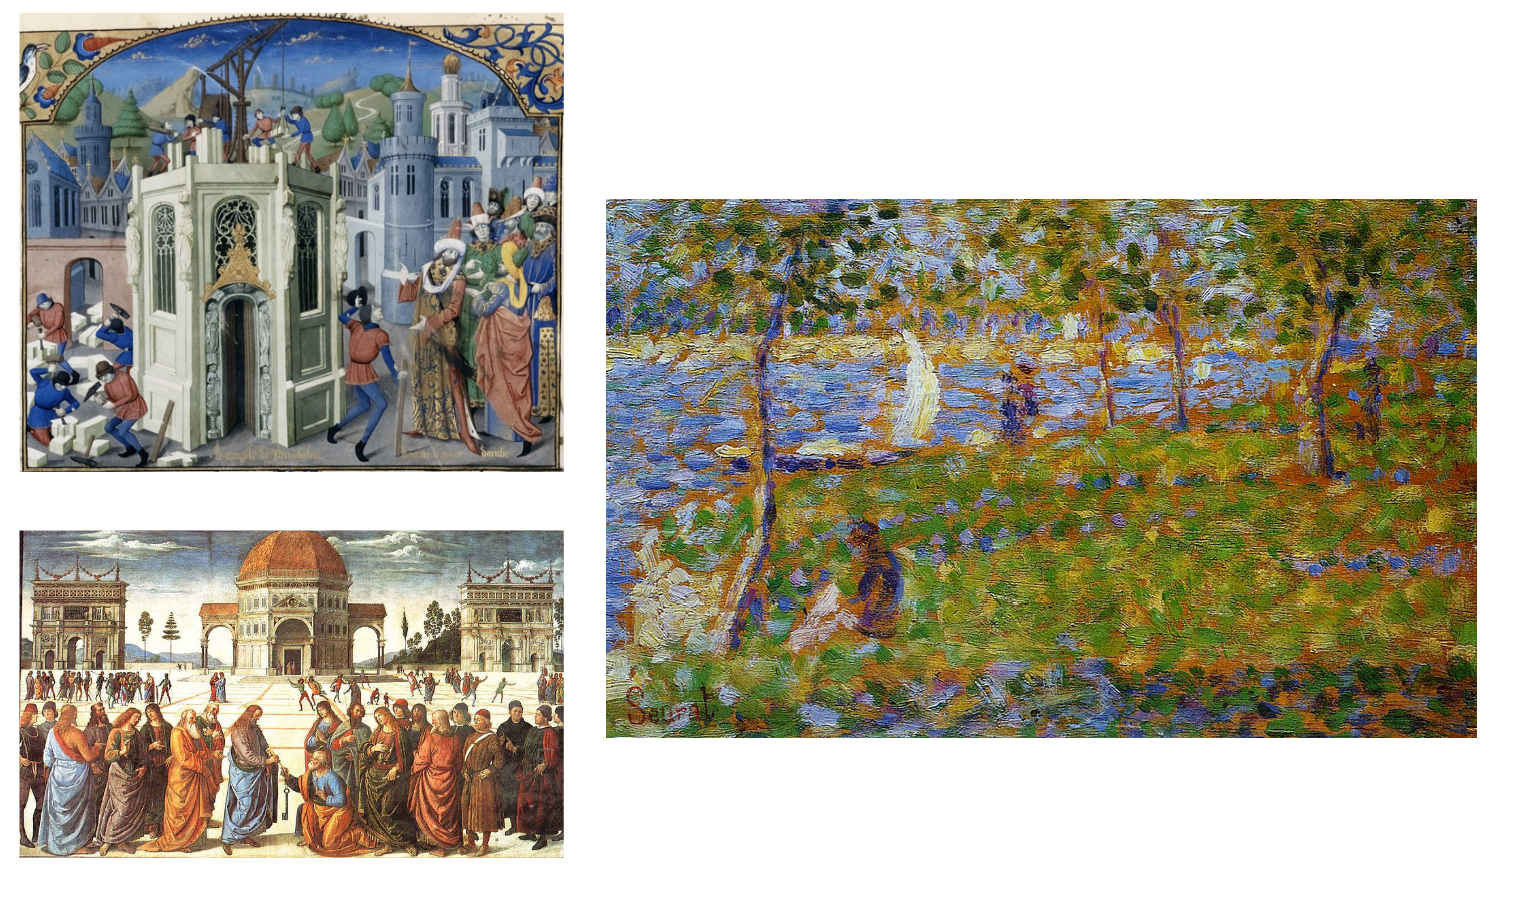
\includegraphics[width=0.9\textwidth]{figs/fig_perspec1.png}
%   \end{center}
%   \caption{Evolução da perspectiva: ``Reconstrução do
%         Templo de Jerusalém'', Guilherme de Tiro (1200); Afresco de Pietro
%         Perugino (1481); Pontilhismo de Seurat.%~\cite{figperspec}
%         }
%   \label{fig:perspec}
% \end{figure}

% \end{frame}

\begin{frame}

\begin{figure}
\begin{center}
    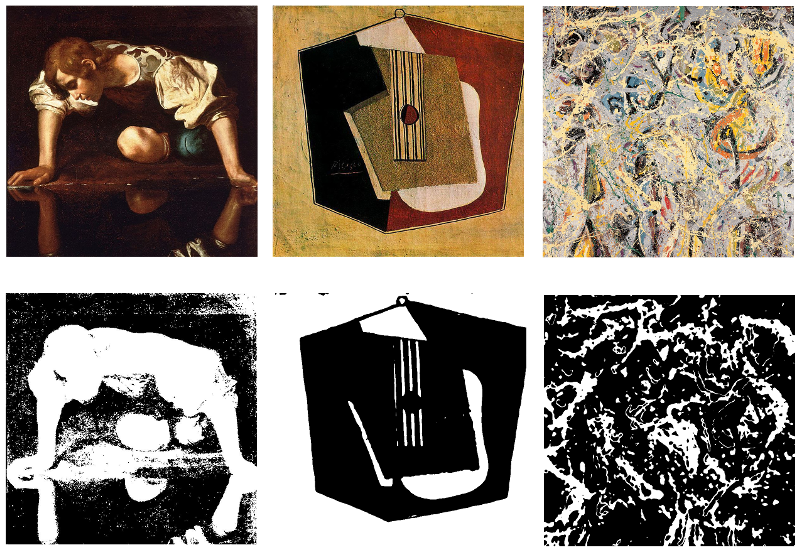
\includegraphics[width=0.9\textwidth]{figs/comp_formas.png}
  \end{center}
  \caption{Evolução da forma: Pinturas de Caravaggio, Picasso e Pollock. \textit{Fonte: Wikipedia}.
        }
  \label{fig:comp_formas}
\end{figure}

\end{frame}

\begin{frame}

\begin{figure}
\begin{center}
    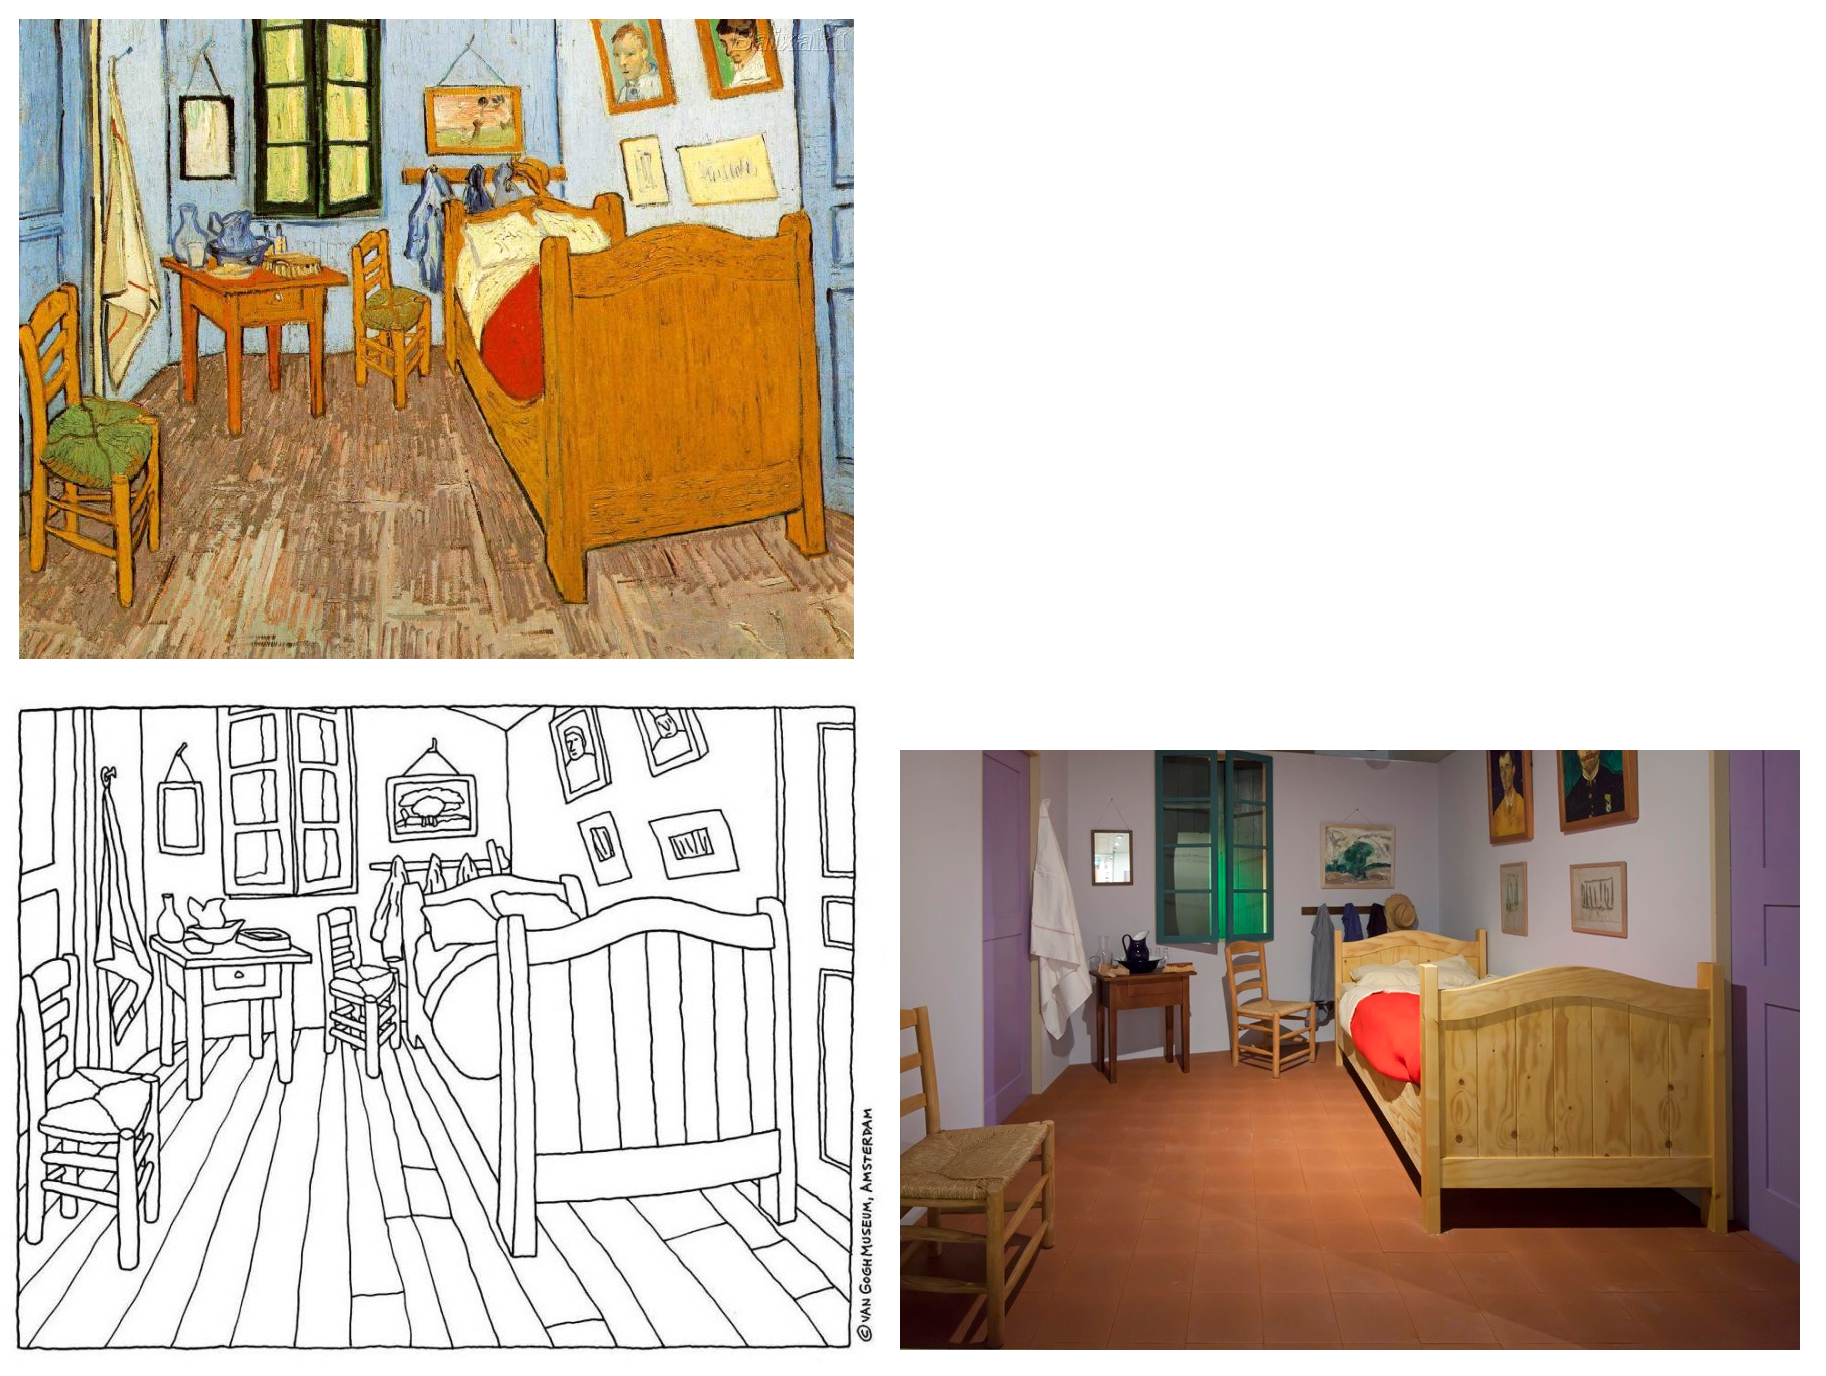
\includegraphics[width=0.75\textwidth]{figs/fig_profundidade1.png}
  \end{center}
  \caption{Evolução da profundidade e proporção: \emph{Quarto em Arles}, Van Gogh (1889). \textit{Fonte: Wikipedia}.}
  \label{fig:profundidade}
\end{figure}

\end{frame}

\begin{frame}

\begin{figure}
\begin{center}
    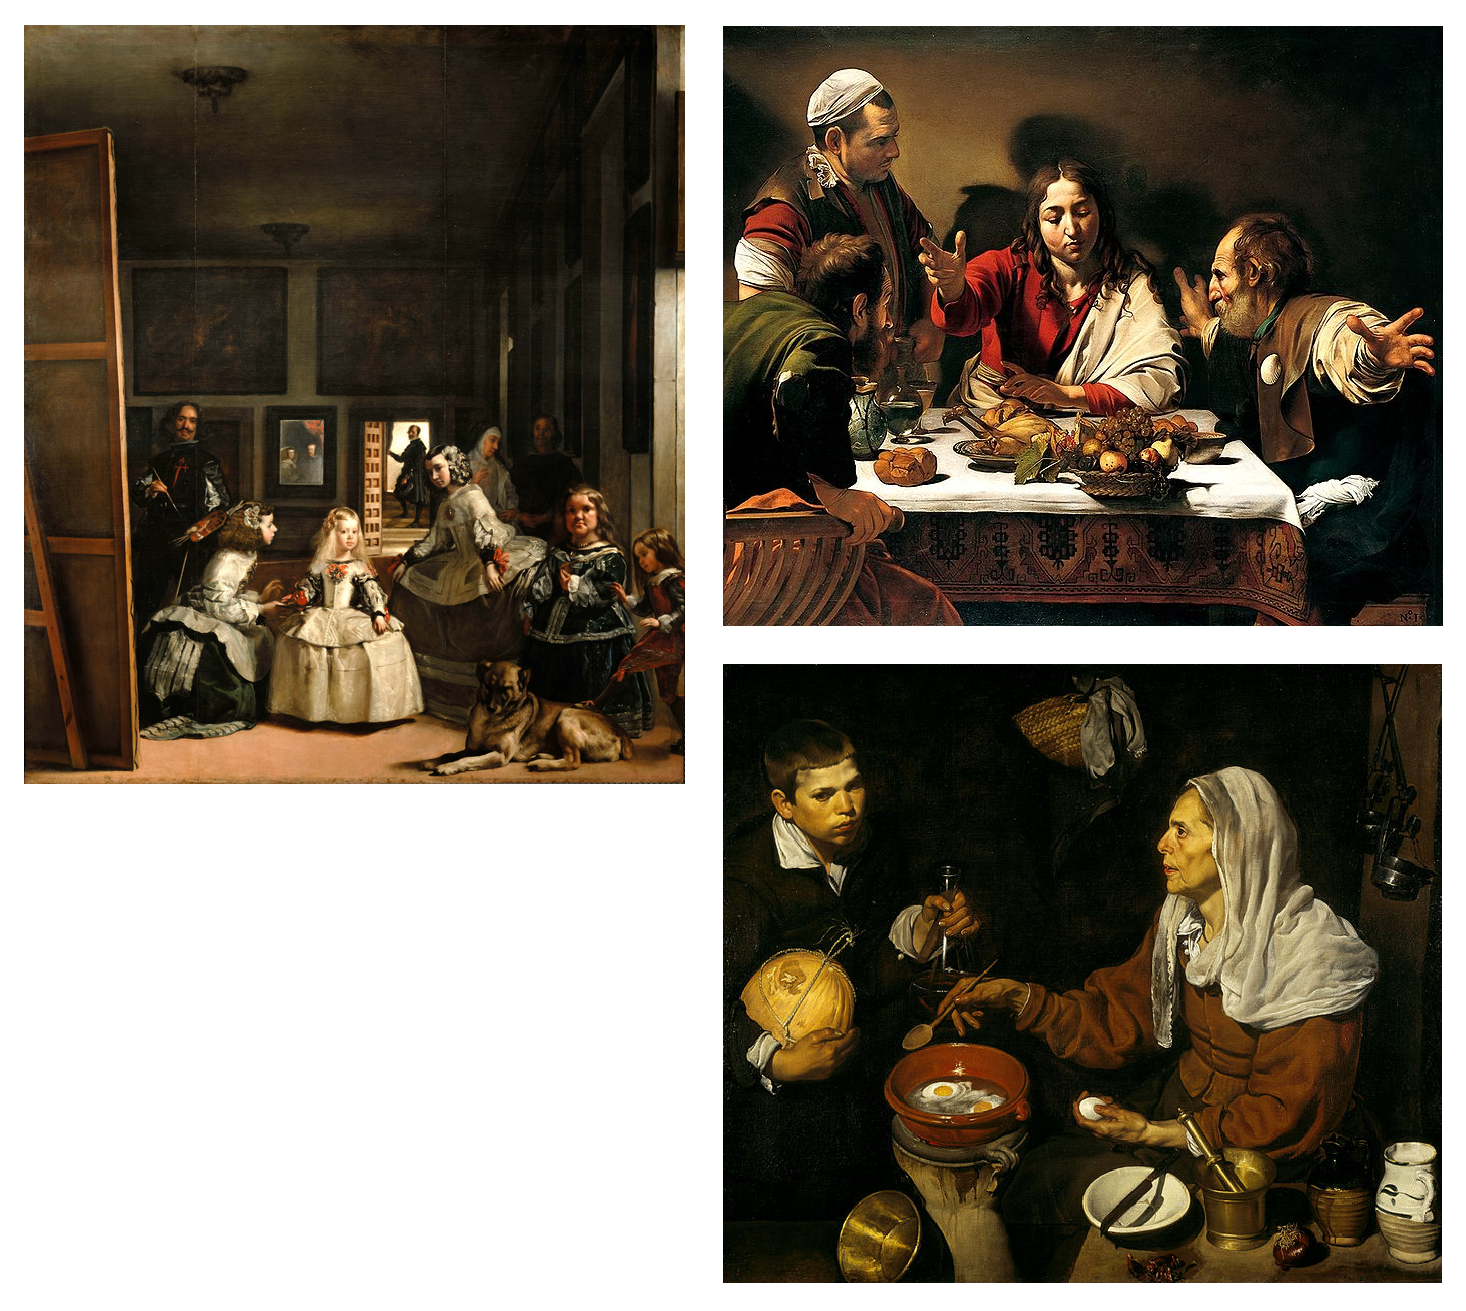
\includegraphics[height=0.55\textwidth]{figs/fig_car_vel.png}
  \end{center}
  \caption{Evolução da intensidade de luz (\textit{chiaroscuro}): Pinturas de Caravaggio e Velázquez. \textit{Fonte: Wikipedia}.}
  \label{fig:carvel}
\end{figure}

\end{frame}

%% motivacao
\subsection{Motivação}
\begin{frame}{Motivação}
\setstretch{1.5}
\begin{itemize}
  \item Estas diferenças e semelhanças possibilitam este estudo.
  \item É possível analisá-las de forma quantitativa?
  \item Confirma ou refuta a História da Arte?
\end{itemize}

\end{frame}

% objetivos
\subsection{Objetivos}
\begin{frame}{Objetivos}
\setstretch{1.5}
\begin{itemize}
  \item Analisar a evolução de estilos artísticos de maneira quantitativa.
  \pause
  \item Empregar conceitos qualitativos (e.g.\ dialética) de maneira quantitativa.
  \pause
  \item Interpretar a análise quantitativa, comparando-a com a História das Artes.
\end{itemize}

\end{frame}

% metodologia
\subsection{Metodologia}
\begin{frame}{Metodologia}
\setstretch{1.5}
\begin{itemize}
  \item Escolha de representantes de dois períodos distintos.
  \pause
  \item Construção de uma base de dados de pinturas.
  \pause
  \item Processamento de imagens para extração de características.
  \pause
  \item Seleção das melhores características.
  \pause
  \item Confirmação por LDA.
  \pause
  \item Cálculo de medidas de oposição, inovação e dialética.
  \pause
  \item Interpretação com base na História da Arte.
\end{itemize}

\end{frame}

% caso de estudo

\section{Caso de estudo}

\subsection{Base de imagens}
\begin{frame}{Base de imagens}
\setstretch{1.5}
  \begin{itemize}
    \item Período Barroco e de movimentos da Arte Moderna.
    \item 6 pintores de cada período, 12 ao total
    \item 20 obras de cada pintor, 240 ao total.
    \item Referenciam períodos marcantes na história de cada artista (e.g.\ Picasso $\to$ Cubismo).
  \end{itemize}

\end{frame}

\subsection{Artistas escolhidos}
\begin{frame}{Artistas escolhidos}

\begin{table}[h!]
\begin{center}
\caption{\label{tab:painters} Pintores escolhidos para a análise, exibidos em
  ordem cro\-no\-ló\-gi\-ca.}
\resizebox{\textwidth}{!}{
\begin{tabular}{l|l|l}
\hline \hline

 \textbf{Artistas}                      & \textbf{Estilos} & \textbf{Período} \\ 
 
 \hline

 Caravaggio                    & Barroco & 1593 - 1610 \\
 Frans Hals                    & Barroco, Idade de ouro Holandesa & 1620 - 1660\\
 Nicolas Poussin               & Barroco, Classicismo & 1620 - 1660\\
 Diego Velázquez           & Barroco & 1618 - 1660\\
 Rembrandt                     & Barroco, Idade de ouro Holandesa, Realismo & 1632 - 1650\\
 Johannes Vermeer              & Barroco, Idade de ouro Holandesa & 1632 - 1670\\
 
 \hline
 
 Vincent van Gogh              & Pós-Impressionismo & 1888 - 1890\\
 Wassily Kandinsky             & Expressionismo, Arte abstrata & 1922 - 1944\\
 Henri Matisse                 & Modernismo, Fauvismo & 1904 - 1910\\
 Pablo Picasso                 & Cubismo & 1909 - 1912\\
 Joan Miró                 & Surrealismo, Dada & 1922 - 1958\\
 Jackson Pollock               & Expressionismo abstrato & 1947 - 1950\\

\hline \hline
\end{tabular}}

\end{center}
\end{table}

\end{frame}

% \subsection{Amostras de pinturas estudadas}
% \begin{frame}{Amostras de pinturas estudadas}

% \begin{figure}[h!]
%   \begin{center}
%   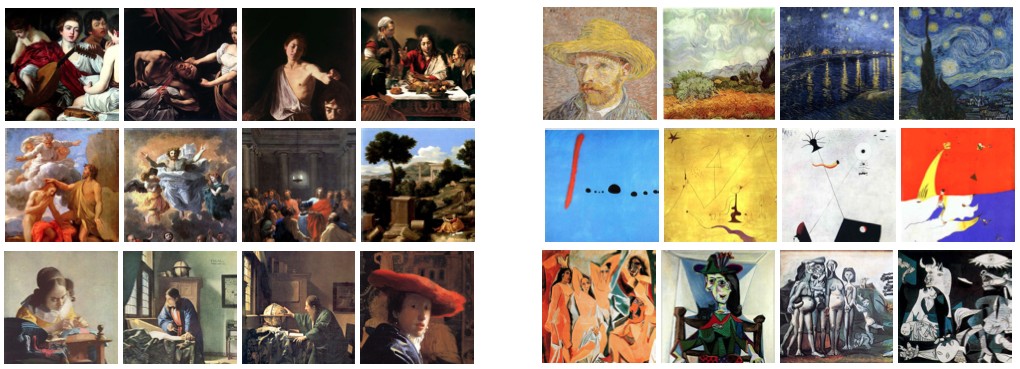
\includegraphics[width=\textwidth]{figs/compara_bar_mod.png} 
% \caption{Amostras de detalhes de pinturas estudadas.}
%     \label{fig:amostra_barroco}
    
      
% \end{center}
% \end{figure}

% \end{frame}

% \subsection{Amostras de pinturas modernas}
% \begin{frame}{Amostras de pinturas modernas}

% \begin{figure}[h!]
%   \begin{center}
%   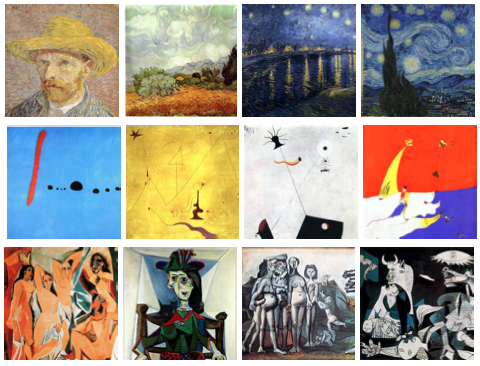
\includegraphics[width=0.8\textwidth]{figs/amostra_moderno} 
% \caption{Amostras de detalhes de pinturas modernas.}
%     \label{fig:amostra_moderno}
    
      
% \end{center}
% \end{figure}

% \end{frame}

% caso de estudo => período barroco

\subsection{Características do Barroco}
\begin{frame}{Características do Barroco}
\setstretch{1.5}
\begin{columns}
 \begin{column}{.49\textwidth}
 \begin{itemize}

\item<1> O Barroco tem como objetivo principal retratar emoções, movimento, o sagrado.

\item<2> Caravaggio é expoente no uso da técnica do
  \textit{chiaroscuro}.

\end{itemize}
 \end{column}

 \begin{column}{.49\textwidth}

\begin{figure}[h!]
  \begin{center}
    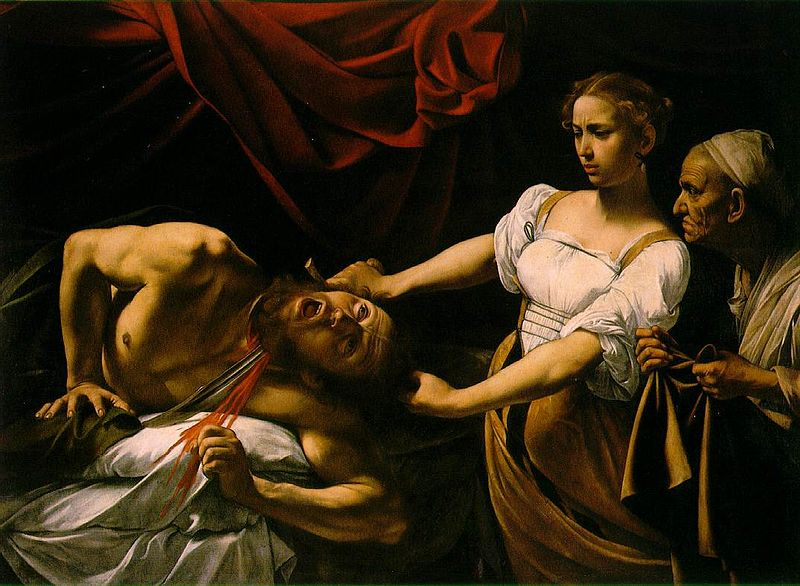
\includegraphics[width=1.0\textwidth]{figs/caravaggio_judite.png}
    \caption{\emph{Judite e Holoferne} (Caravaggio), c. 1599. \textit{Fonte: Wikipedia}.}
    \label{fig:caravaggio:judite}
\end{center}
\end{figure}

\end{column}
\end{columns}
\end{frame}

\begin{frame}{Características do Barroco}

Velázquez e Vermeer se assemelham com Caravaggio pois ambos
  utilizavam \textit{chiaroscuro}.

\begin{figure}[h!]
  \begin{center}
    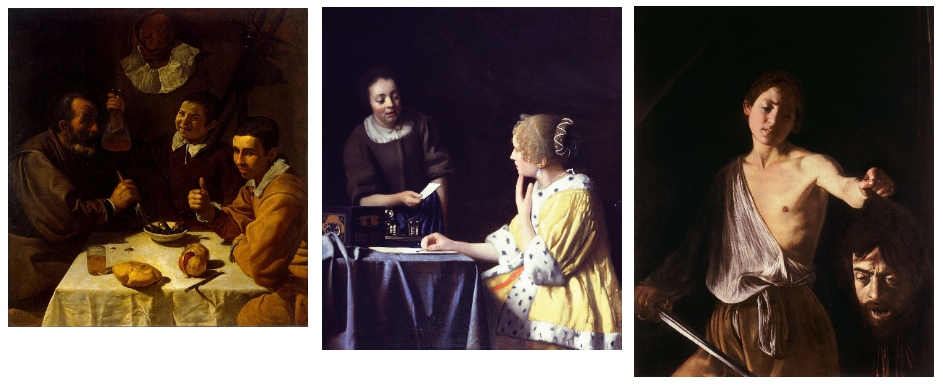
\includegraphics[width=1.0\textwidth]{figs/compara_vel_ver_car.png}
    \caption{Comparação entre pinturas de Velázquez, Vermeer e Caravaggio. \textit{Fonte: Wikipedia}.}
\end{center}
\end{figure}

\end{frame}

\begin{frame}{Características do Barroco}

Poussin se opõe à Caravaggio: ele não deseja retratar a verdade, 
mas sim o belo (influências de Carracci, Reni e Rafael).

\begin{figure}[h!]
  \begin{center}
    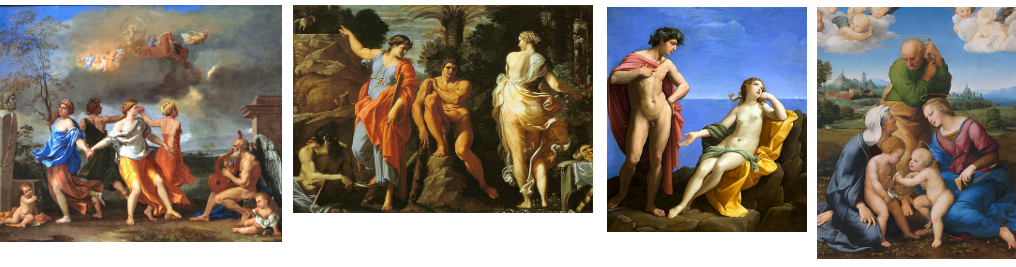
\includegraphics[width=1.0\textwidth]{figs/compara_poussin.png}
    \caption{Comparação entre pinturas de Poussin, Carracci, Reni e Rafael. \textit{Fonte: Wikipedia}.}
\end{center}
\end{figure}

\end{frame}

% caso de estudo => movimentos da arte moderna

\subsection{Características da Arte Moderna}

\begin{frame}{Características da Arte Moderna}
  
  Pintores modernos são, em geral, independentes em estilo. Barrocos compartilham estilos
  tradicionais.

  \begin{figure}[h!]
  \begin{center}
    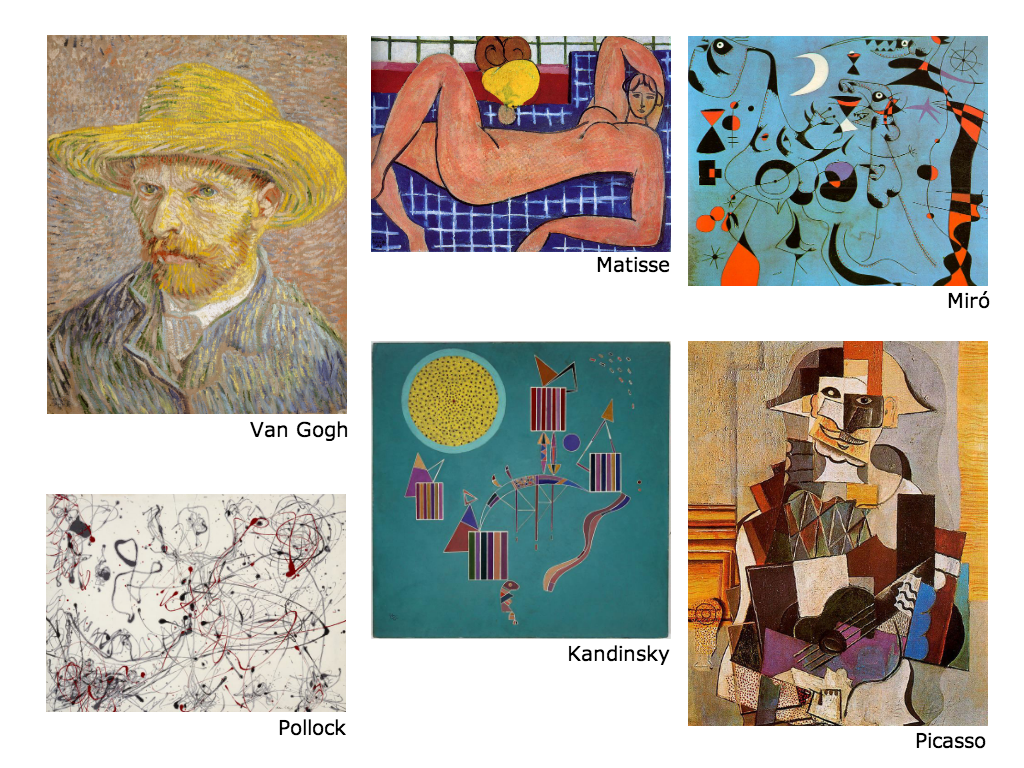
\includegraphics[width=0.65\textwidth]{figs/compara_moderno2.png}
    \caption{Comparação entre pinturas modernas. \textit{Fonte: Wikipedia}.}
\end{center}
\end{figure}

\end{frame}

\begin{frame}{Características da Arte Moderna}

  Diferença cronológica e estética entre o Barroco
  e os movimentos da Arte Moderna.

  \begin{figure}[h!]
  \begin{center}
    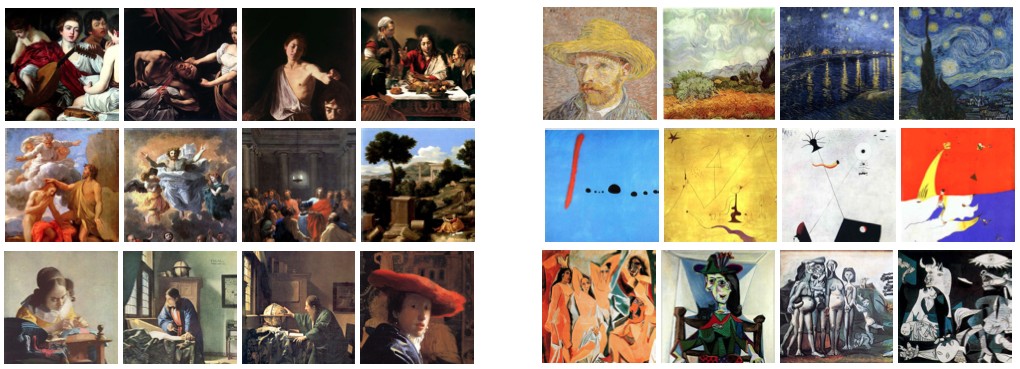
\includegraphics[width=1.0\textwidth]{figs/compara_bar_mod.png}
    \caption{Comparação entre pinturas barrocas e modernas. \textit{Fonte: Wikipedia}.}
\end{center}
\end{figure}

\end{frame}

\begin{frame}{Características da Arte Moderna}

  Pollock apresenta pinturas que diferem de todos os outros
  pintores escolhidos.

  \begin{figure}[h!]
  \begin{center}
  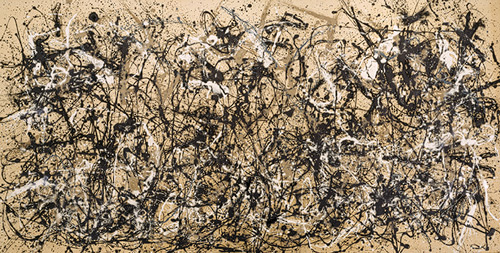
\includegraphics[width=0.9\textwidth]{figs/pollock_ritmo.png}
  \caption{\emph{Ritmo de Outono} (Jackson Pollock), c. 1950. \textit{Fonte: Wikipedia}.}
  \label{fig:pollock:ritmo}
  \end{center}
\end{figure}

\end{frame}

\subsection{Sumário de características}
\begin{frame}{Sumário de características}

\begin{table}[h]

  \begin{center}
\caption{\label{tab:caracarts} Sumário de características do período Barroco e de cada artista dos movimentos da Arte Moderna estudados.}
 \resizebox{\textwidth}{!}{%

\begin{tabular}{|l|ll|}
\hline \hline
\textbf{Barroco}                                                                                                                   & \multicolumn{2}{l|}{\textbf{Arte Moderna}}                                                                                                                               \\ \hline
\multirow{6}{*}{\begin{tabular}[c]{@{}l@{}}Contraste (e.g. claro-escuro); \\ emoção ao invés da razão; movimento; \\ dramaticidade; sensualidade; \\ beleza; fantasia; \\ a verdade; o sagrado\end{tabular}} & Van Gogh  & \begin{tabular}[c]{@{}l@{}}Sensação; movimento; textura; cores; \\ uso da perspectiva e profundidade de uma \\ nova maneira; distorção\end{tabular} \\ \cline{2-3} 
                                                                                                                          & Kandinsky & \begin{tabular}[c]{@{}l@{}}Abstrato; cromatismo; \\ interpretação psicológica; \\ formas geométricas, puras\end{tabular}                            \\ \cline{2-3} 
                                                                                                                          & Matisse   & \begin{tabular}[c]{@{}l@{}}Cores ``violentas''; desprezo às formas \\ naturais; decoração; simplicidade\end{tabular}                                \\ \cline{2-3} 
                                                                                                                          & Picasso   & \begin{tabular}[c]{@{}l@{}}Solidez; simplicidade; formas geométricas; \\ colagem de várias perspectivas\end{tabular}                                \\ \cline{2-3} 
                                                                                                                          & Miró      & \begin{tabular}[c]{@{}l@{}}Surreal; automatismo; símbolos e seus \\ significados; negação das técnicas de \\ pintura existentes\end{tabular}        \\ \cline{2-3} 
                                                                                                                          & Pollock   & Abstrato; pintura de ação, pura, espontânea                                                                                                         \\ \hline \hline
\end{tabular}
}
\end{center}

\end{table}

\end{frame}

% análise das pinturas

\section{Análise das pinturas}

\subsection{Etapas para processamento das imagens}
\begin{frame}{Etapas para processamento das imagens}

\begin{figure}[ht!]
\begin{center}
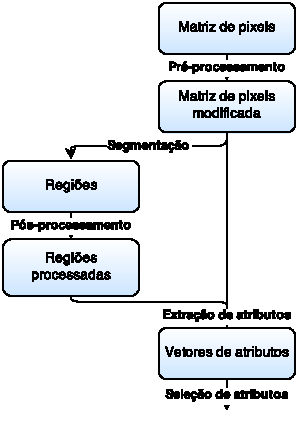
\includegraphics[scale=0.8]{figs/etapas_pdi2} 
\caption{Etapas para processamento das pinturas.}
\label{fig:etapas-pdi}
        
\end{center}
\end{figure}

\end{frame}

\subsection{Janelamento}
\begin{frame}{Janelamento}

\begin{columns}
 \begin{column}{.49\textwidth}
 Imagens foram recortadas em janelas de $800 \times 800$ \textit{pixels}.
 \end{column}

 \begin{column}{.49\textwidth}

\begin{figure}[h!]
\begin{center}
  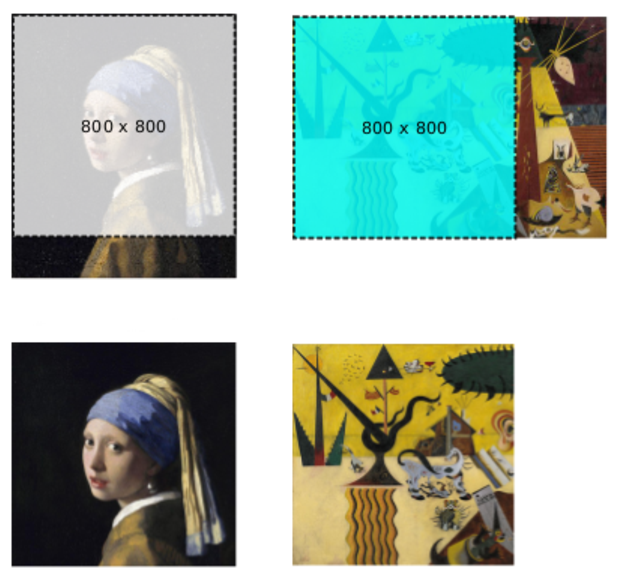
\includegraphics[width=\columnwidth]{figs/passos_janelamento2}
        \caption{Exemplos de janelamento.}
        \label{fig:janelamento}
\end{center}
\end{figure}

\end{column}
\end{columns}

\end{frame}

\subsection{Pré-processamento}
\begin{frame}{Pré-processamento}

 \begin{itemize}
    \item<1> Equalização por histograma para ajustar o nível de contraste das imagens.

    \item<2> Filtro por mediana para suavização, porém preservando detalhes de borda.
  \end{itemize}

\begin{figure}[h!]
\begin{center}
  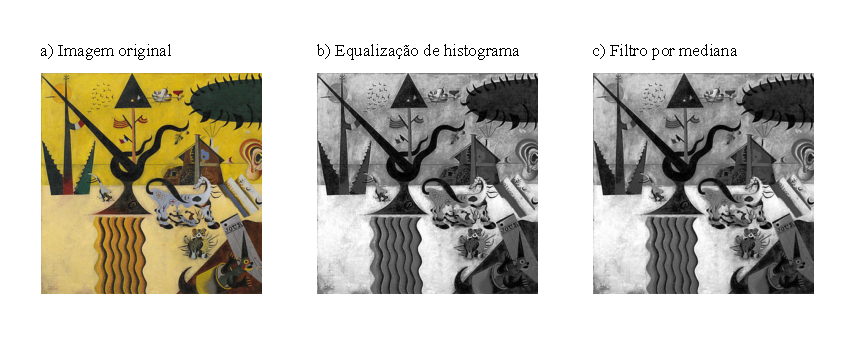
\includegraphics[width=.9\textwidth]{figs/passos_eq}
         \caption{Pré-processamento utilizando equalização de histograma
        e filtro por mediana.}
        \label{fig:eq}
\end{center}
\end{figure}

\end{frame}

\subsection{Segmentação}
\begin{frame}{Segmentação}
\setstretch{1.5}
  \begin{itemize}
    \item{ Comparação empírica entre métodos.
      \begin{itemize}
        \item Watershed;
        \item Felzenswald;
        \item SLIC (\textit{Simple Linear Iterative Clustering}).%~\cite{slic}
      \end{itemize}
    }
    \pause
    \item Aplicação de SLIC com $k=10$ (número de \textit{clusters}).
    \pause
    \item $k>10$ não revelaram bons resultados.
  \end{itemize}

\end{frame}

\begin{frame}{Segmentação}

  \begin{figure}[h!]
\begin{center}
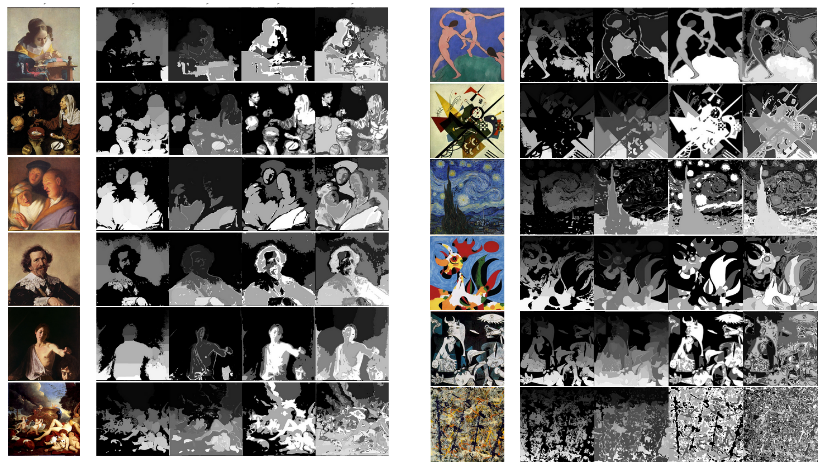
\includegraphics[scale=.35]{figs/compara_segmentacao}
        \caption{Experimentos realizados para segmentação de
        pinturas. Imagem original; Watershed; Felzenswald; SLIC com $k=10$; SLIC com $k=20$.} 
         \label{fig:expsegs} 
\end{center}
\end{figure}

\end{frame}

\subsection{Pós-processamento}

\begin{frame}{Rotulação e remoção de imperfeições}

  \begin{itemize}
    \item<1> Rotulação das regiões conexas.
    %\pause
    \item<2> Remoção de ``buracos'': operação morfológica binária de fechamento.
    %\pause
    \item<3> Remoção de ruídos: filtro de áreas $< \theta$.
  \end{itemize}

\begin{figure}[h!]
\begin{center}
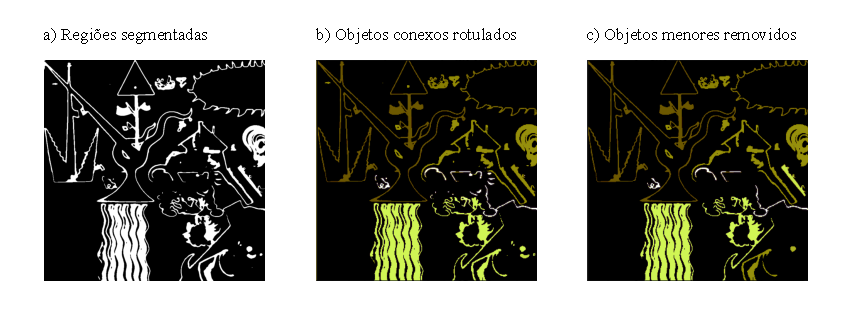
\includegraphics[scale=0.8]{figs/passos_rotulacao}
          \caption{Etapas de pós-processamento.}
        \label{fig:rotulacao}
\end{center}
\end{figure}

\end{frame}

% análise das pinturas => características extraídas

\subsection{Atributos extraídos}

\begin{frame}{Atributos extraídos (das imagens)}
 
    \textbf{Atributos espectrais} através do cálculo de densidade espectral para as imagens e colunas, linhas e centróides das imagens.

\begin{table}
  \begin{center}
  
 \resizebox{\textwidth}{!}{%
  \begin{tabular}{l|l}
    \hline \hline
    \textbf{$\mathcal{A}_i$} & \textbf{Descrição} \\
    \hline  

    %%>>
$\mathcal{A}_1$ & 
    Média das energias nas linhas $x$ da imagem em tons de cinza \\
    %$\mathcal{A}_1  = \frac{\sum_j E_{(i,j)}}{N_j}$ \\

    $\mathcal{A}_2$ &
    Desvio padrão das energias nas linhas $x$ da imagem em tons de cinza \\
    %$\mathcal{A}_2 = \sqrt{\frac{\sum_j (E_{(i,j)} - \mu)^2}{N_j}}$ \\

    $\mathcal{A}_3$ &
    Média das energias nas colunas $y$ da imagem em tons de cinza \\
    %$\mathcal{A}_3 = \frac{\sum_i E_{(i,j)}}{N_i}$ \\

    $\mathcal{A}_4$ &
    Desvio padrão das energias nas colunas $y$ da imagem em tons de cinza \\
    %$\mathcal{A}_4 = \sqrt{\frac{\sum_i (E_{(i,j)} - \mu)^2}{N_i}}$ \\

    $\mathcal{A}_5$ &
    Centroide das energias nas linhas $x$ da imagem em tons de cinza \\
    %$\mathcal{A}_5 = \frac{\sum_j j E_{(i,j)}}{N_j}$ \\

    $\mathcal{A}_6$ &
    Centroide das energias nas colunas $y$ da imagem em tons de cinza \\
    %$\mathcal{A}_6 = \frac{\sum_i i E_{(i,j)}}{N_i}$ \\

    $\mathcal{A}_7$ &
    Média das energias nas linhas $x$ e colunas $y$ da imagem em tons de cinza \\
    %$\mathcal{A}_7 = \frac{\sum E_{(i,j)}}{N_i + N_j}$ \\

    $\mathcal{A}_8$ &
    Desvio padrão das energias nas linhas $x$ e colunas $y$ da imagem em tons de
    cinza \\
    %$\mathcal{A}_8 = \sqrt{\frac{\sum (E_{(i,j)} - \mu)^2}{N_i + N_j}}$ \\

    $\mathcal{A}_{9-16}$ &
    As mesmas medidas $\mathcal{A}_{1-8}$ mas aplicadas à banda vermelha da
    imagem \\

    $\mathcal{A}_{17-24}$ &
    As mesmas medidas $\mathcal{A}_{1-8}$ mas aplicadas à banda verde da
    imagem \\

    $\mathcal{A}_{25-32}$ &
    As mesmas medidas $\mathcal{A}_{1-8}$ mas aplicadas à banda azul da
    imagem \\
    %%<<  

     \hline
    \end{tabular}}

  \end{center}
\end{table}

\end{frame}

\begin{frame}{Atributos extraídos (das imagens)}
 
    \textbf{Atributos de textura e complexidade} por 14 medidas de Haralick.%~\cite{haralick}

\begin{table}
  \begin{center}
  
 \resizebox{\textwidth}{!}{%
  \begin{tabular}{l|l}
    \hline \hline
    \textbf{$\mathcal{A}_i$} & \textbf{Descrição} \\
    \hline  

    %%>>
$\mathcal{A}_{33-46}$ &
    As 14 medidas de textura de Haralick para a direção $\beta = 0^o$ ou $\vec{d} = (1, 0)$ \\

$\mathcal{A}_{47-60}$ &
    As 14 medidas de textura de Haralick para a direção $\beta = 45^o$ ou $\vec{d} = (1, 1)$ \\

$\mathcal{A}_{61-74}$ &
    As 14 medidas de textura de Haralick para a direção $\beta = 90^o$ ou $\vec{d} = (0, 1)$ \\

$\mathcal{A}_{75-88}$ &
    As 14 medidas de textura de Haralick para a direção $\beta = 135^o$ ou $\vec{d} = (-1, 1)$ \\
    %%<<  

     \hline
    \end{tabular}}

  \end{center}
\end{table}

\end{frame}

\begin{frame}{Atributos extraídos (das regiões conexas)}
 
    \textbf{Atributos de contorno e forma} pelo cálculo da curvatura das regiões conexas; sua área e perímetro, assim como área e perímetro da região convexa (obtida por \textit{convex-hull}).%~\cite{luciano}

\only<1>{
  \begin{figure}[h!]
\begin{center}
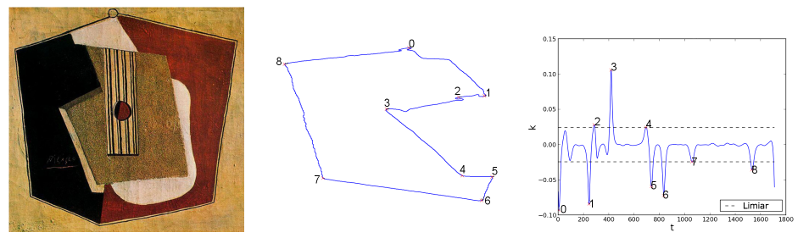
\includegraphics[width=.9\textwidth]{figs/curvatura}
          \caption{Cálculo de curvatura.}
        \label{fig:calccurvatura}
\end{center}
\end{figure}
}

\only<2>{
\begin{table}
  \begin{center}
  
 \resizebox{\textwidth}{!}{%
  \begin{tabular}{l|l}
    \hline \hline
    \textbf{$\mathcal{A}_i$} & \textbf{Descrição} \\
    \hline  

    %%>>
$\mathcal{A}_{89}$ &
    Média das distâncias (euclidiana) entre os picos de curvatura \\

    $\mathcal{A}_{90}$ &
    Desvio padrão das distâncias (euclidiana) entre os picos de curvatura \\

    $\mathcal{A}_{91}$ &
    Média das distâncias (em \textit{pixels} do contorno) entre os picos de curvatura \\

    $\mathcal{A}_{92}$ &
    Desvio padrão das distâncias (em \textit{pixels} do contorno) entre os picos de
    curvatura \\

    $\mathcal{A}_{93}$ &
    Quantidade de picos de curvatura \\

    $\mathcal{A}_{94}$ &
    Perímetro da curvatura \\

    $\mathcal{A}_{95}$ &
    Área da região conexa \\

    $\mathcal{A}_{96}$ &
    Razão entre o perímetro e a área da região \\

    $\mathcal{A}_{97}$ &
    Quantidade de segmentos de uma pintura \\

    $\mathcal{A}_{98}$ &
    Área da região convexa \\

    $\mathcal{A}_{99}$ &
    Razão entre a área da região convexa e a área da região conexa original \\
    %%<<  

     \hline \hline
    \end{tabular}}

  \end{center}
\end{table}    
}
\end{frame}

% análise das pinturas => escolha das melhores características

%%%% SELECAO DE FISCHER EXPLICAR E CURVATURA
\subsection{Seleção de atributos}
\begin{frame}{Seleção de atributos}

  \begin{itemize}
    \item Cálculo da razão de Fisher entre todos os pares $(a,b)$ de atributos para as $240$ pinturas e $12$ classes.
    \pause
    \item Matriz $S_{intra}$ determina o espalhamento intra-classe.
    % \begin{equation}
    % S_{intra} = \sum_{i=1}^K S_i
    % \end{equation}
    \pause
    \item Matriz $S_{inter}$ determina o espalhamento inter-classe.
    % \begin{equation}
    % S_{inter} = \sum_{i=1}^K N_i(\vec{\mu_i} - \vec{M})(\vec{\mu_i} - \vec{M})^T
    % \end{equation}
    \pause
%     Sendo $N_i$ o número de amostras para a classe $C_i$ e a matriz de
% espalhamento para a classe $C_i$ definida como
%     \begin{equation}
%     S_i = \sum_{i \in C_i} (\vec{f_i} - \vec{\mu_i})(\vec{f_i} - \vec{\mu_i})^T
%     \end{equation}
    \item O traço da razão entre as matrizes resulta na razão de Fisher $\alpha$.
    \begin{equation} \label{eq:alpha}
    \alpha = \mathrm{tr}(S_{inter} S_{intra}^{-1})
    \end{equation}
  \end{itemize}

\end{frame}

\begin{frame}{Seleção de atributos}

\begin{table}[ht] \footnotesize
  \begin{center}
  \caption{\label{tab:alpha} Melhores pares $(a,b)$ de atributos
    segundo
    $\alpha$.}
 \resizebox{\textwidth}{!}{%
 \begin{tabular}{@{}llll}
 \hline \hline
 \textbf{Par} & \textbf{Atributo $a$}    & \textbf{Atributo $b$}   & \textbf{$\alpha$} \\ 
 
 \hline
 
 1 & \textbf{média do número de picos} & \textbf{média do número de segmentos} & \textbf{42.445} \\
 2 & média do número de segmentos & média da área de convex-hull & 37.406 \\
 3 & média do perímetro do segmento & média do número de segmentos & 36.703 \\
 4 & média da área do segmento & média do número de segmentos & 36.214 \\
 5 & média do número de segmentos & média área convexa / área total & 34.885 \\
 6 & média de circularidade ($\mathrm{Per.}^2/\mathrm{Area}$) & média do número
 de segmentos & 33.540 \\
 7 & média da energia das linhas (canal verde) & média do número de segmentos & 32.954 \\
 8 & média da energia das linhas e colunas (canal verde) & média do número de segmentos & 32.954 \\
 9 & d.p. da energia das linhas (canal verde) & média do número de segmentos & 32.932 \\
 10 & d.p. da energia das linhas e colunas (canal verde) & média do número
 de segmentos & 32.906 \\
 11 & média de entropia local (janela de dimensão 5) & média do número de segmentos & 32.898 \\
 12 & entropia (Haralick adj. 4) & média do número de segmentos & 32.898 \\
 13 & entropia (Haralick adj. 3) & média do número de segmentos & 32.883 \\
 14 & entropia (Haralick adj. 1) & média do número de segmentos & 32.874 \\
 15 & entropia (Haralick adj. 2) & média do número de segmentos & 32.869 \\
 16 & média da energia das linhas (canal vermelho) & média do número de segmentos & 32.865 \\
\hline \hline
 \end{tabular}}
\end{center}
\end{table}

\end{frame}

% resultados => resultados para melhores atributos

\section{Resultados}

\subsection{Resultados para melhores atributos}
\begin{frame}{Resultados para melhores atributos}

\only<1>{
\begin{figure}[h!]
\begin{center}

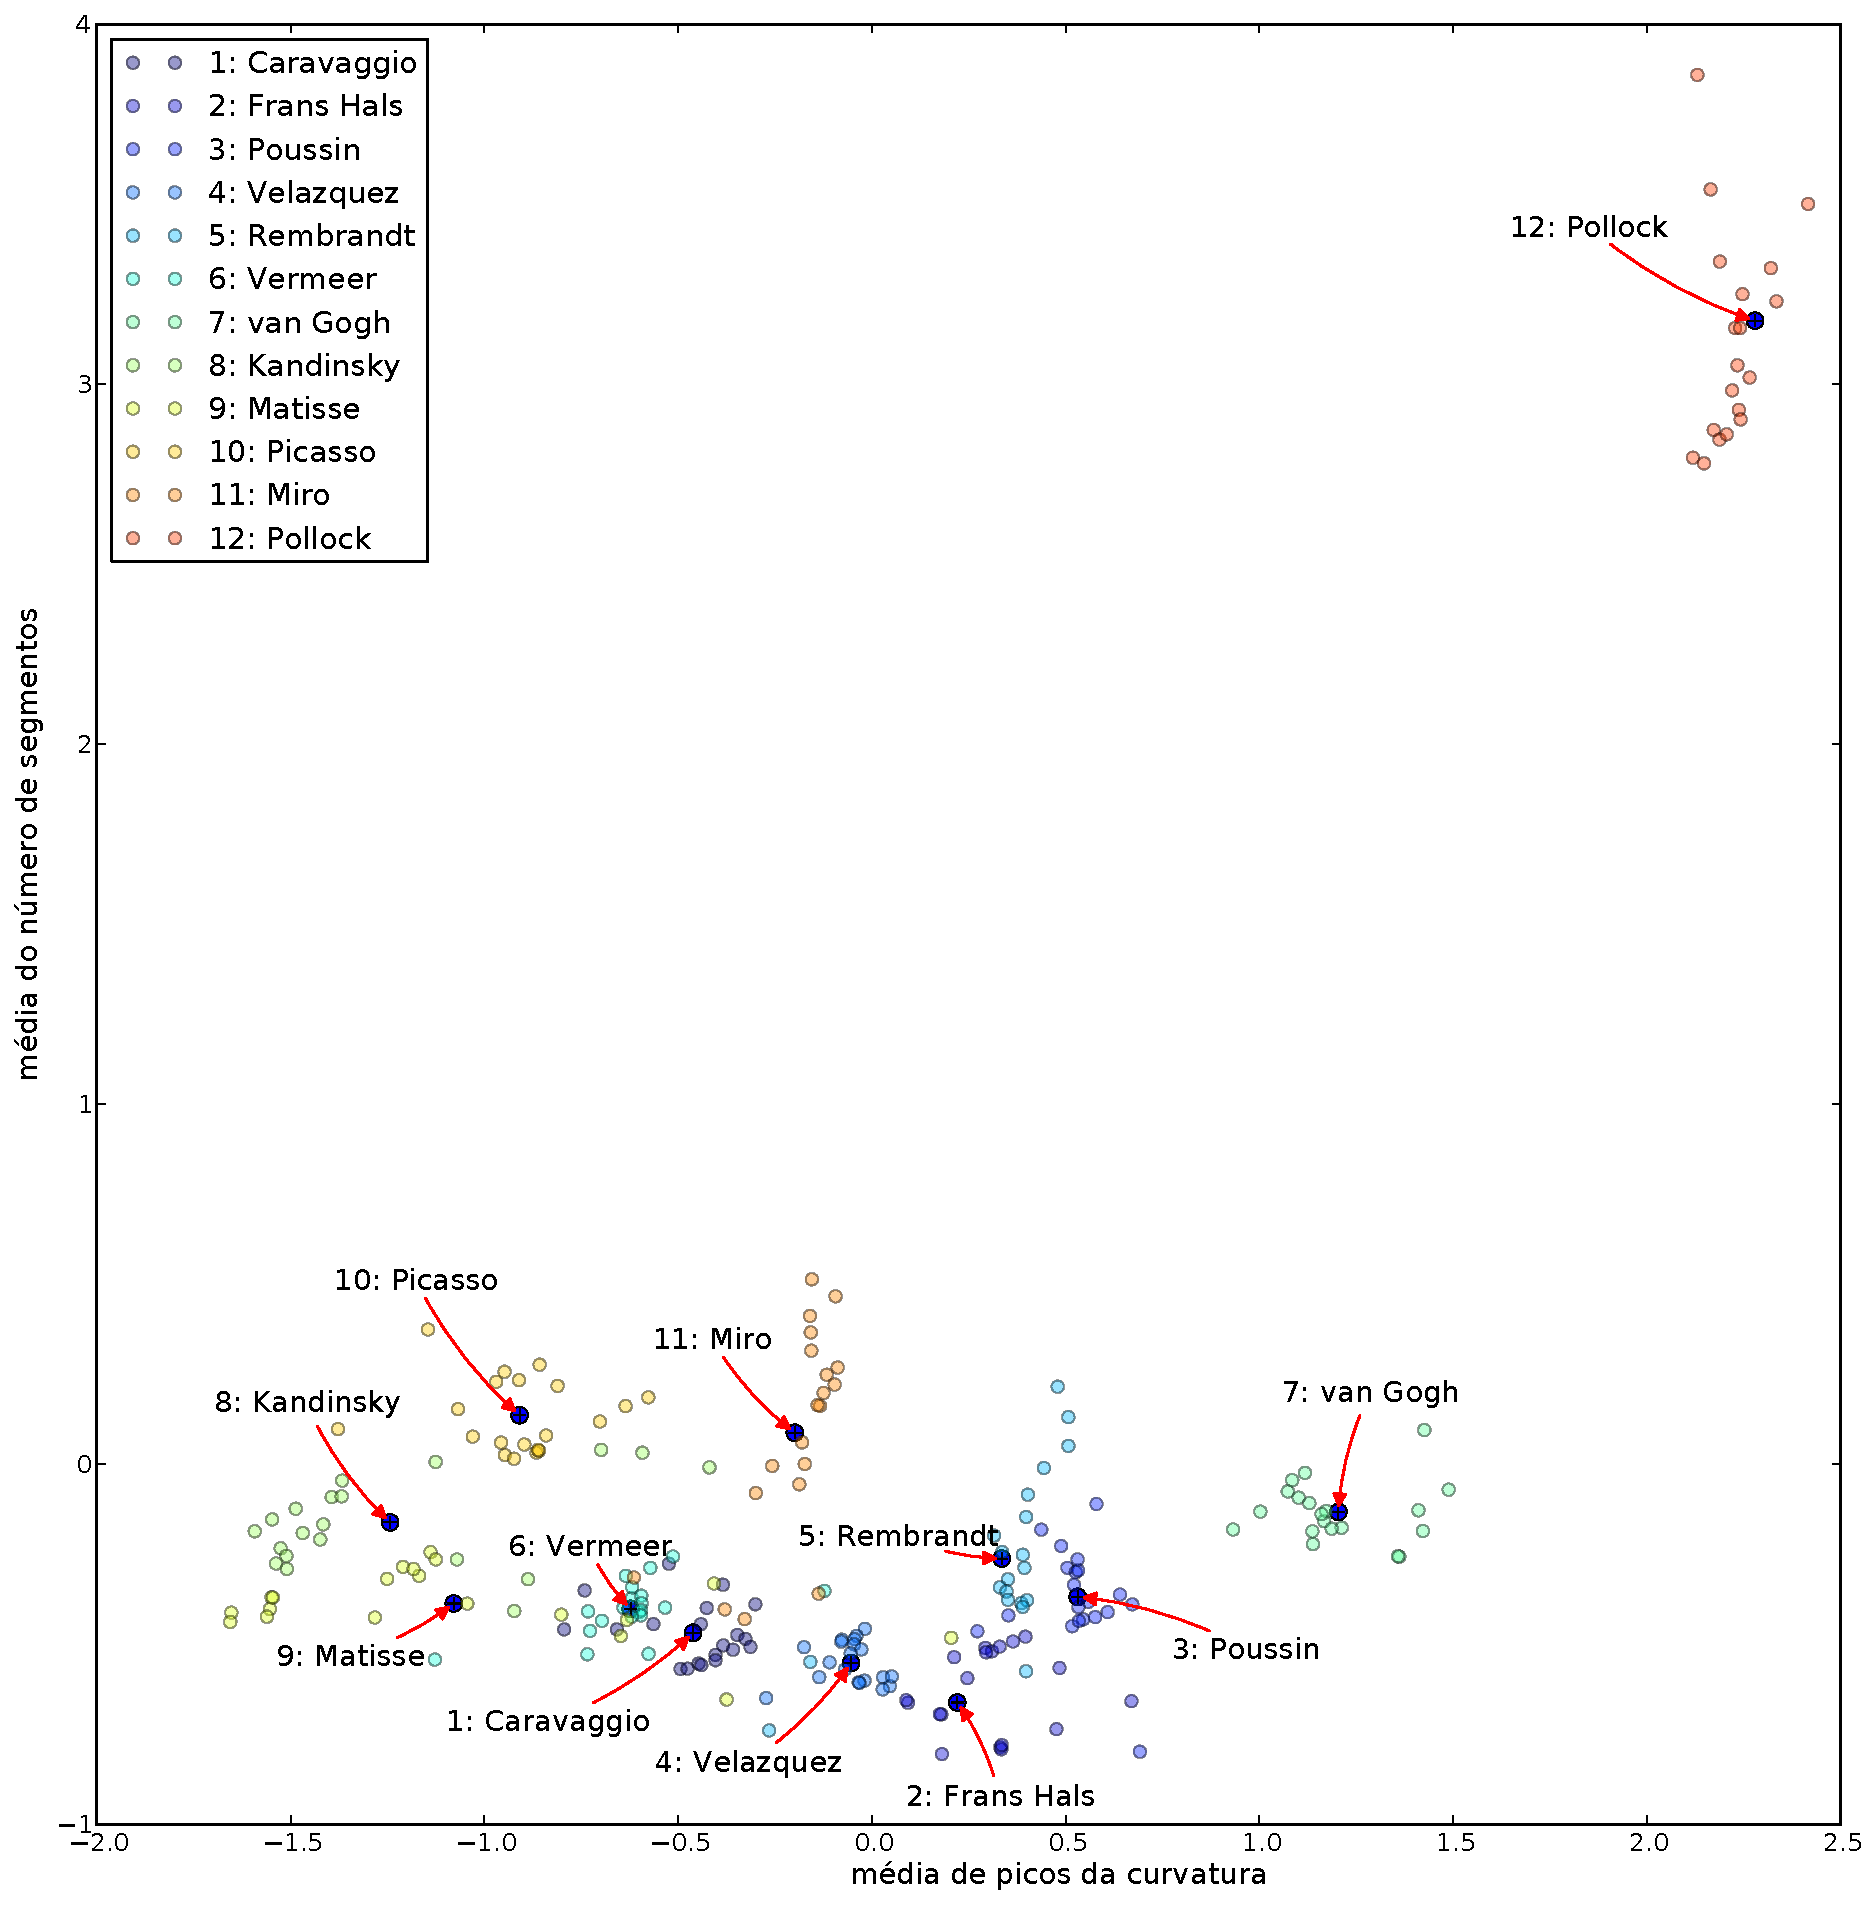
\includegraphics[width=.55\textwidth]{figs/caso1_g1}
      \caption{Projeção do \textit{espaço criativo} considerando \emph{média de picos da curvatura} e
        \emph{média do número de segmentos}.}
        \label{fig:caso1_g1}
        
       
\end{center}
\end{figure}
}

\only<2>{
\begin{figure}[h!]
\begin{center}

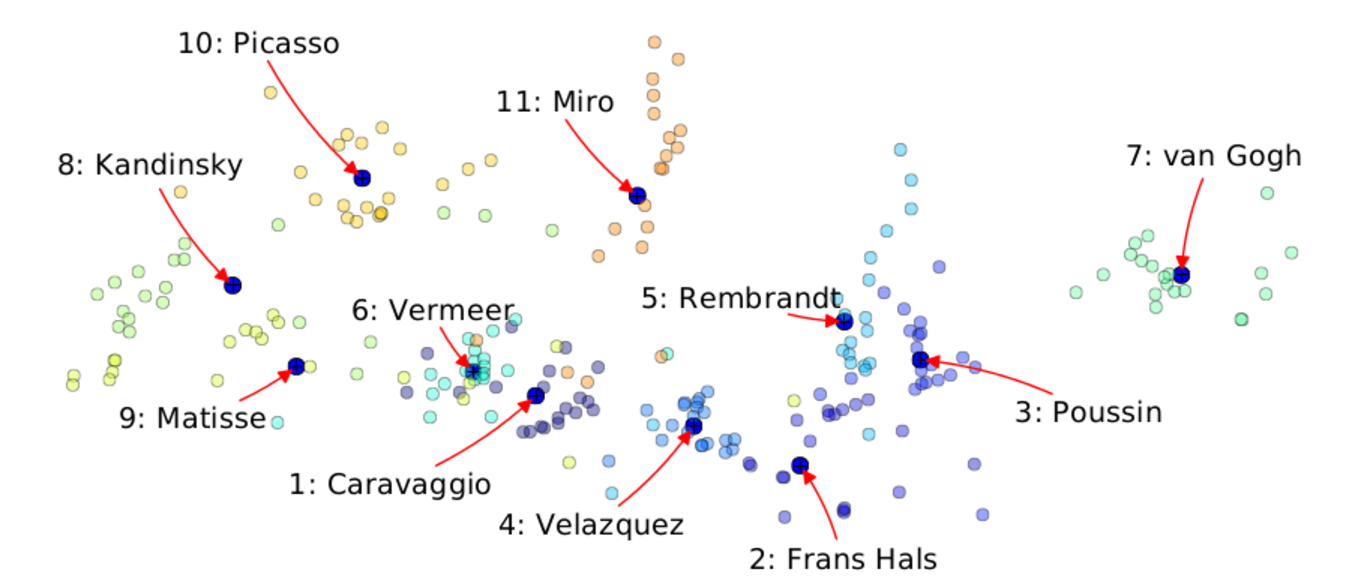
\includegraphics[width=.9\textwidth]{figs/caso1_g1_zoom1}
      \caption{Detalhe da projeção.}
        \label{fig:caso1_g1_zoom1}
\end{center}
\end{figure}
}

\end{frame}

\begin{frame}{Resultados para melhores atributos}

\only<1>{
\begin{figure}[h!]
\begin{center}
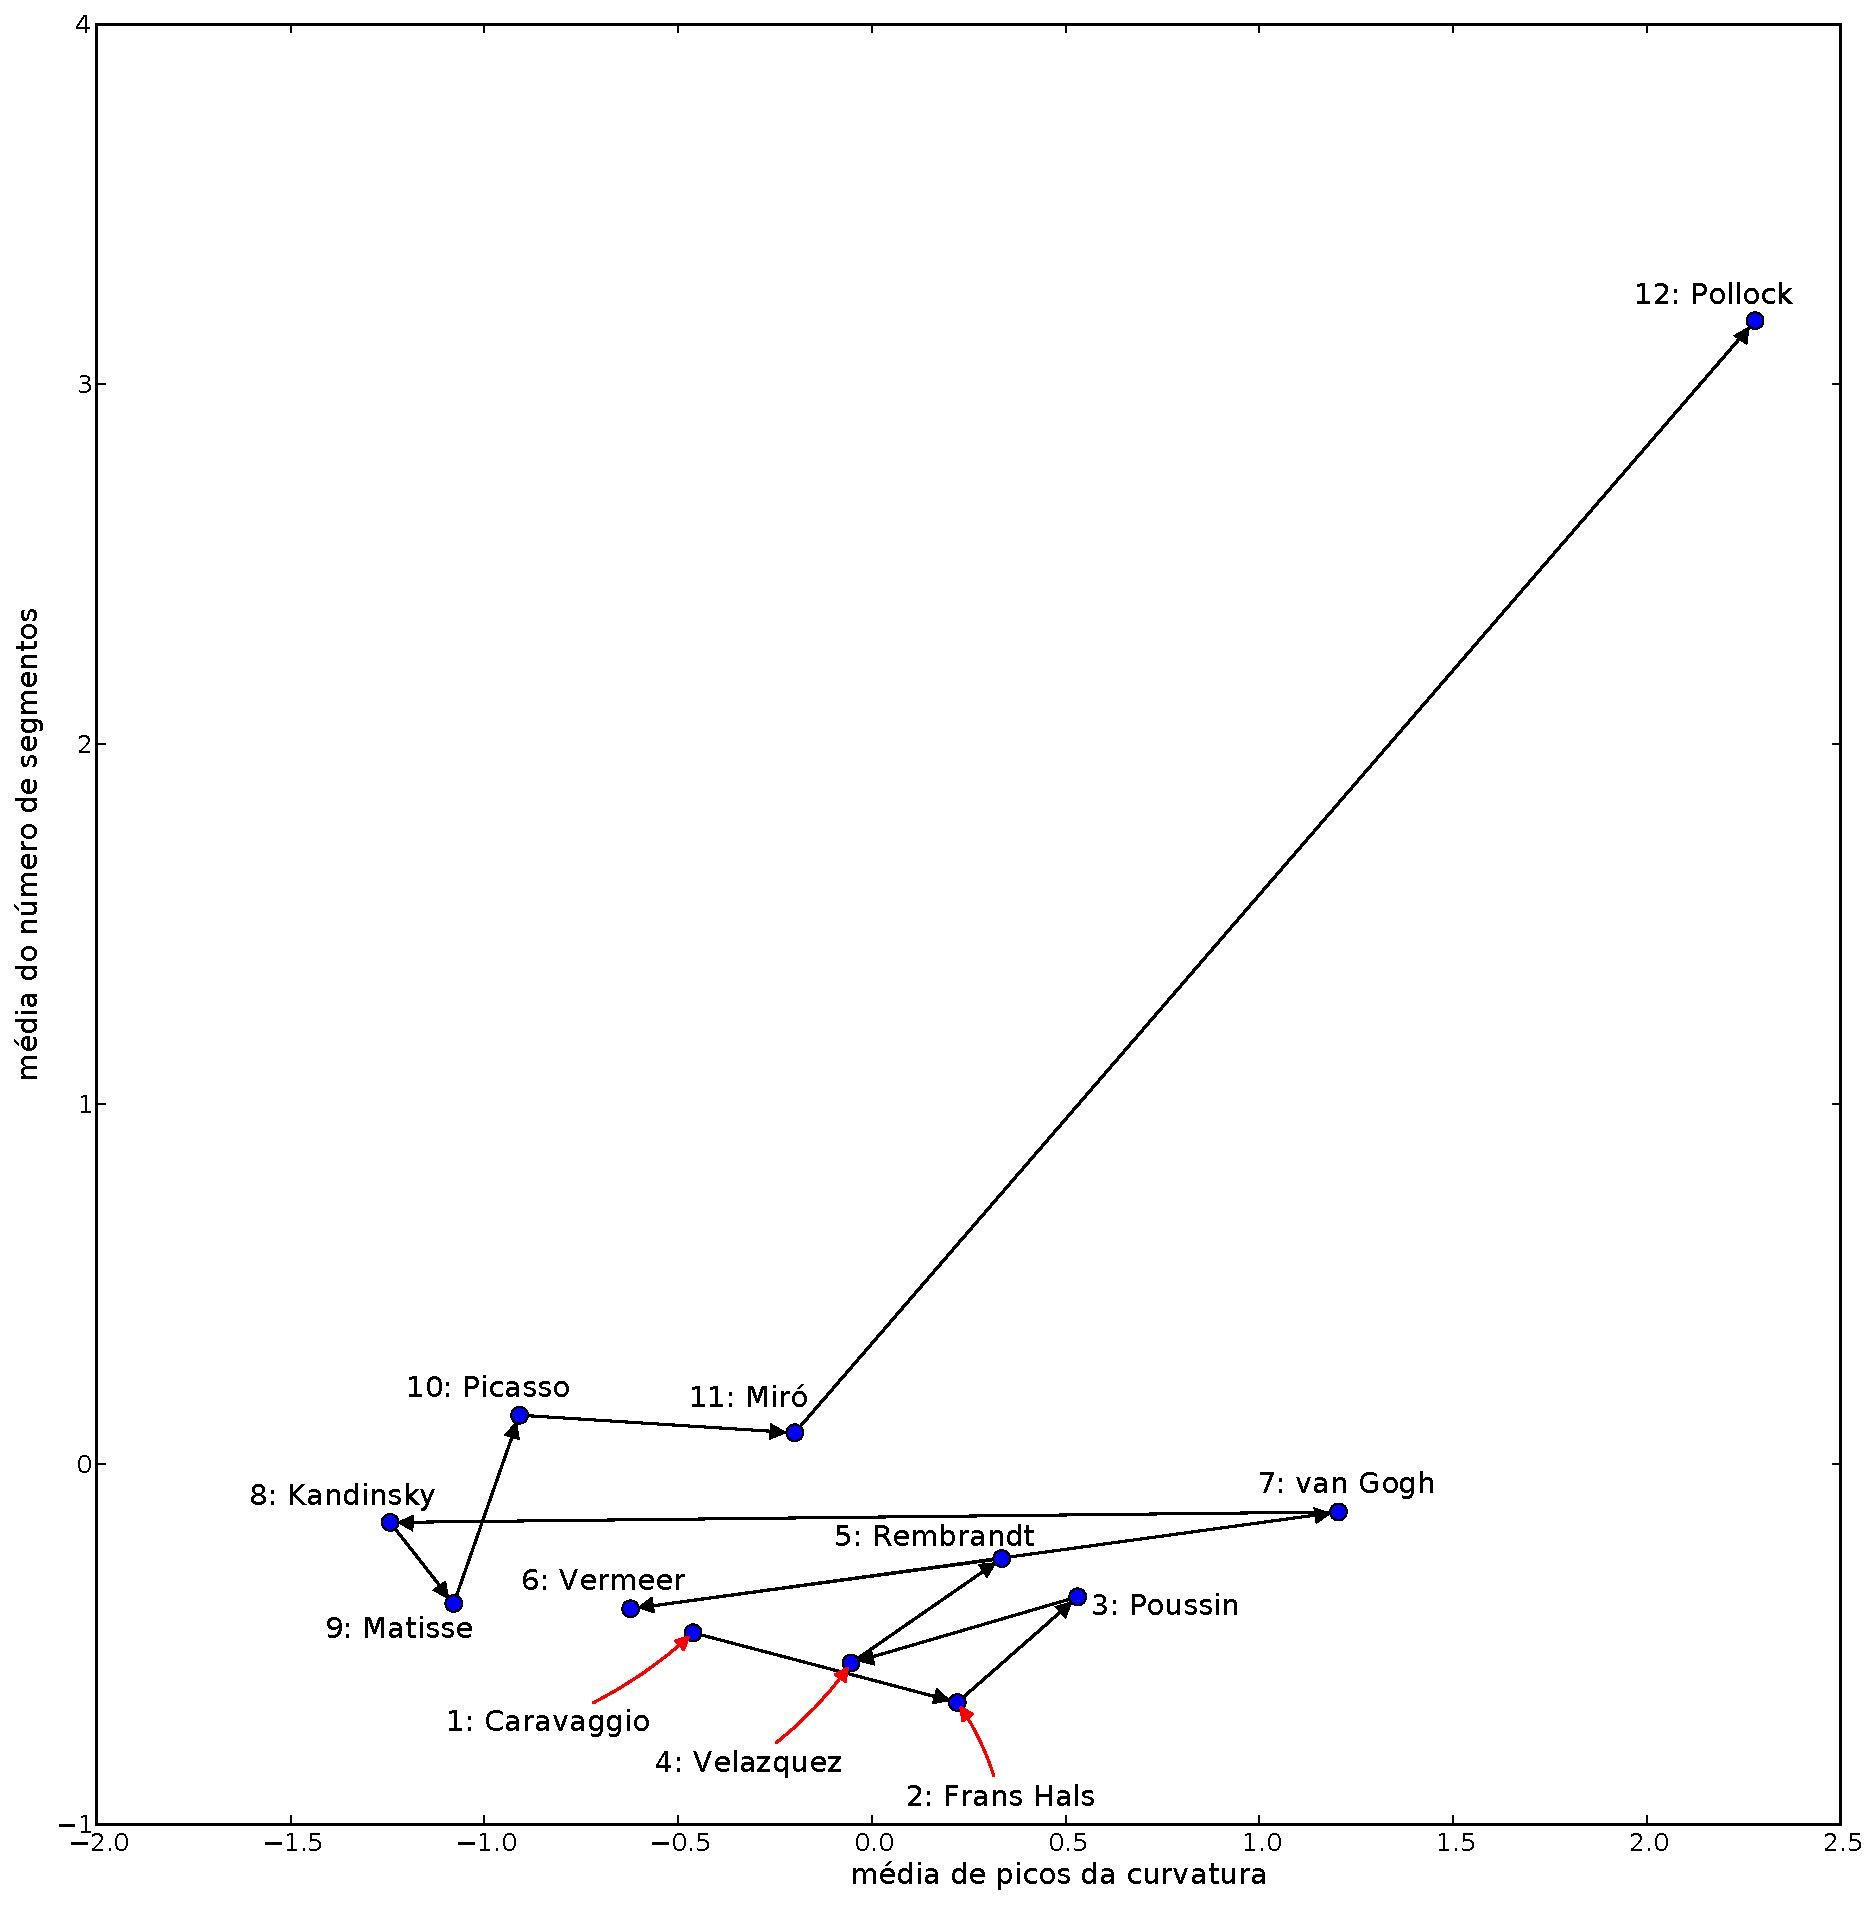
\includegraphics[width=.55\textwidth,keepaspectratio]{figs/caso1_g2}
         \caption{Série temporal considerando
        \emph{média de picos da curvatura} e \emph{média do número de
          segmentos}.}
        \label{fig:caso1_g2}
\end{center}
\end{figure}
}

\only<2>{
\begin{figure}[h!]
\begin{center}

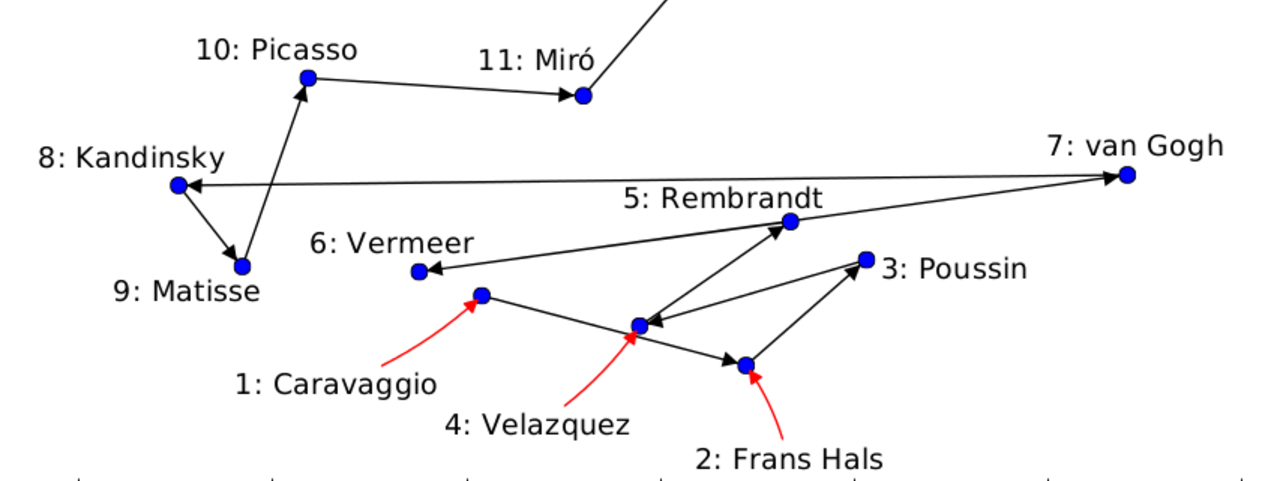
\includegraphics[width=.9\textwidth]{figs/caso1_g2_zoom1}
      \caption{Detalhe da série temporal.}
        \label{fig:caso1_g1_zoom1}
\end{center}
\end{figure}
}

\end{frame}


%%%%%%%%%%%%%%%%%%%%%%%
\subsection{Releitura do Barroco}
\begin{frame}{Releitura do Barroco}

Velázquez e Vermeer se assemelham com Caravaggio pois ambos
  utilizavam \textit{chiaroscuro}.

\begin{figure}[h!]
  \begin{center}
    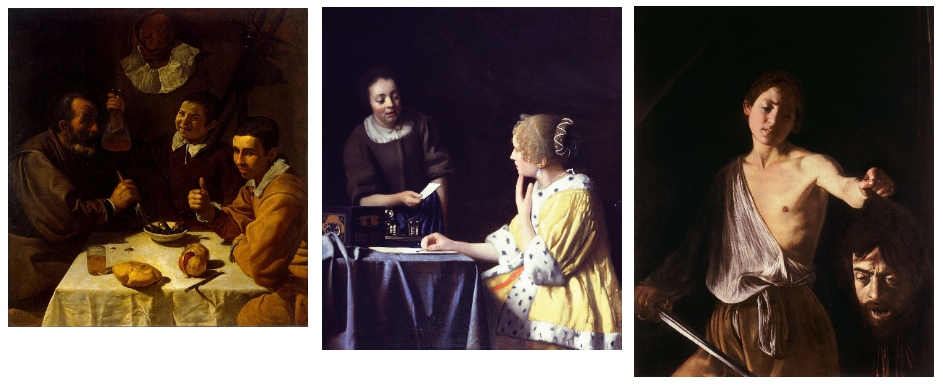
\includegraphics[width=1.0\textwidth]{figs/compara_vel_ver_car.png}
    \caption{Comparação entre pinturas de Velázquez, Vermeer e Caravaggio. \textit{Fonte: Wikipedia}.}
\end{center}
\end{figure}

\end{frame}
\begin{frame}{Releitura do Barroco}

\begin{columns}
 \begin{column}{.49\textwidth}
 \only<1>{
\begin{figure}[h!]
  \begin{center}
    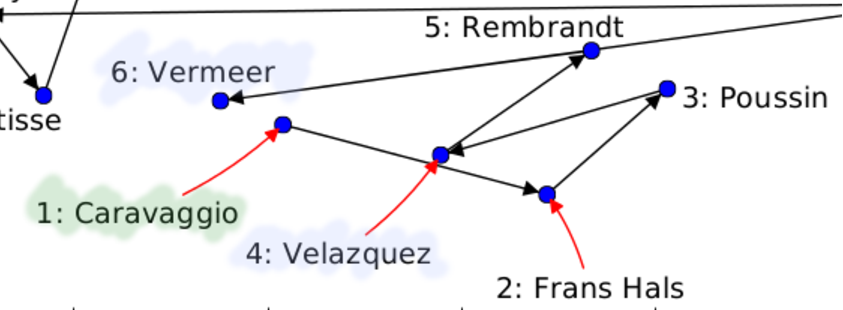
\includegraphics[width=1.2\columnwidth]{figs/caso1_g2_zoom2}
    \caption{Detalhe da série temporal.}
\end{center}
\end{figure}
}
 \only<2>{
\begin{figure}[h!]
  \begin{center}
    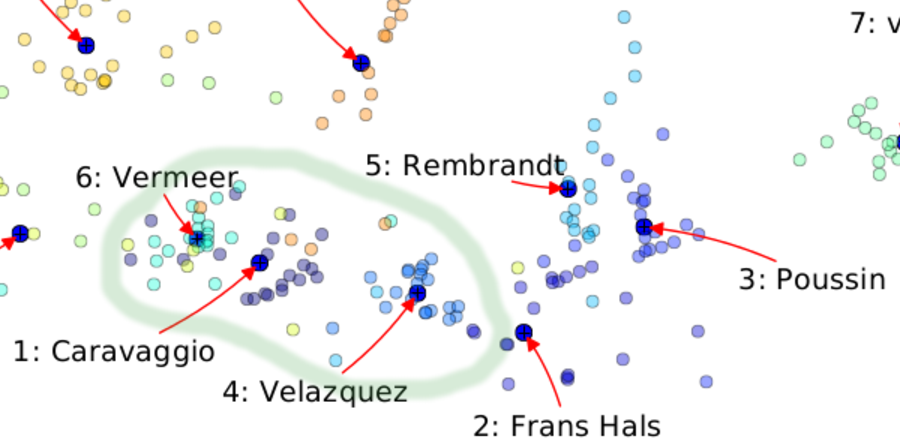
\includegraphics[width=1.2\columnwidth]{figs/caso1_g1_zoom2}
    \caption{Detalhe da projeção.}
\end{center}
\end{figure}
}
 \only<3>{
\begin{figure}[h!]
  \begin{center}
    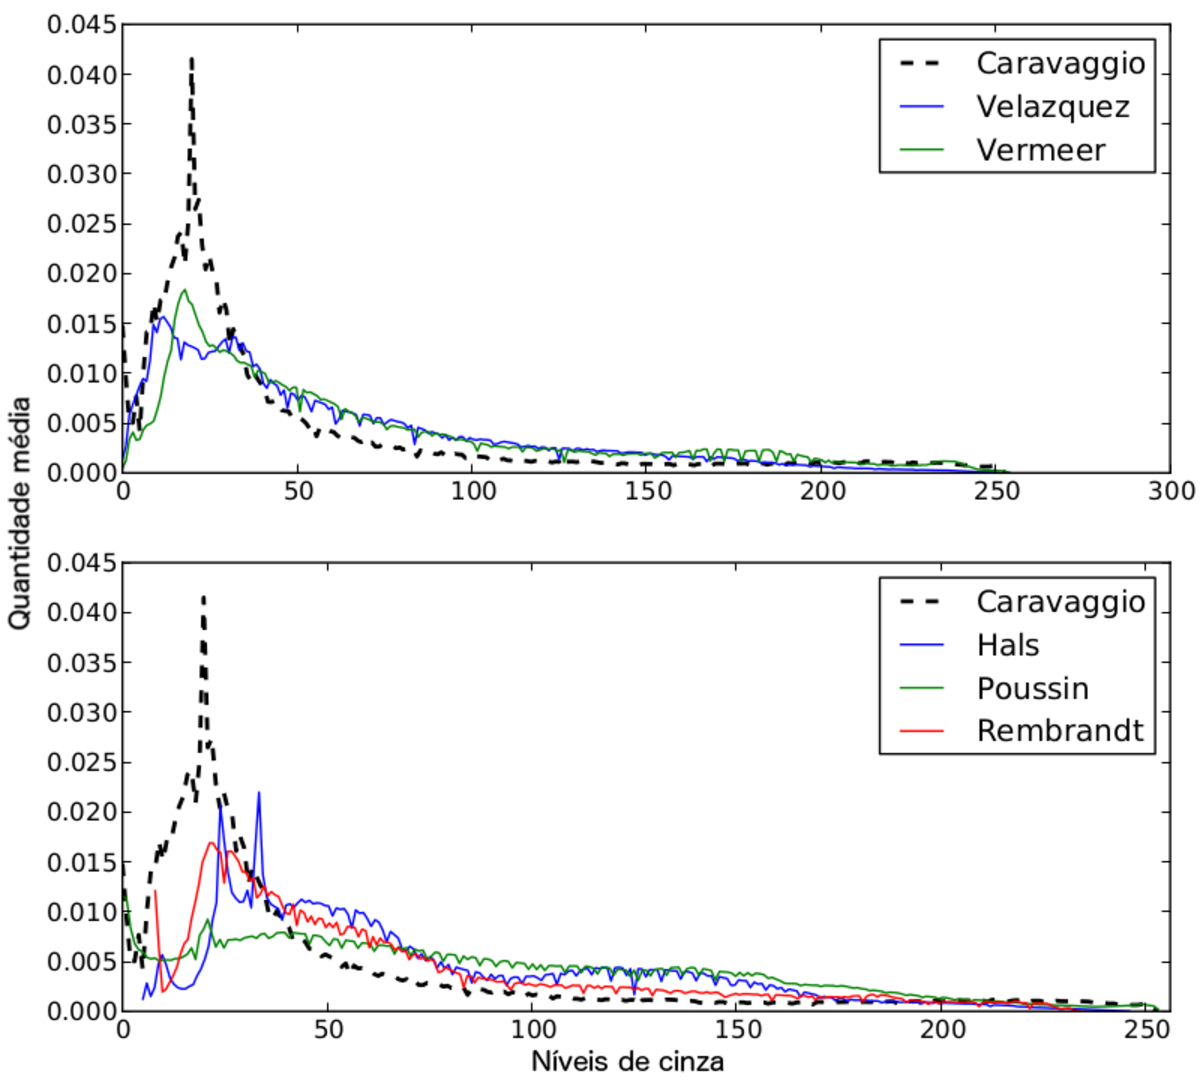
\includegraphics[width=1.1\columnwidth]{figs/chiaroscuro2}
    \caption{Histogramas dos níveis médios de cinza.}
\end{center}
\end{figure}
}
 \end{column}

 \begin{column}{.49\textwidth}
  \begin{itemize}
    \item<1> Velázquez e Vermeer parecem ``voltar'' a Caravaggio.

    \item<2> Sobreposição entre seus clusters.

    \item<3> Similaridade entre seus histogramas de constraste. 

    \item<3> Rembrandt e Frans Hals também possuem similaridade, pois usavam \textit{chiaroscuro}.

    \item<3> Poussin se opõe, suas pinturas são mais claras.
    \end{itemize}
 \end{column}
\end{columns}

\end{frame}

% \begin{frame}{Período Barroco}

%   \begin{figure}[h!]
% \begin{center}
%   { \centering 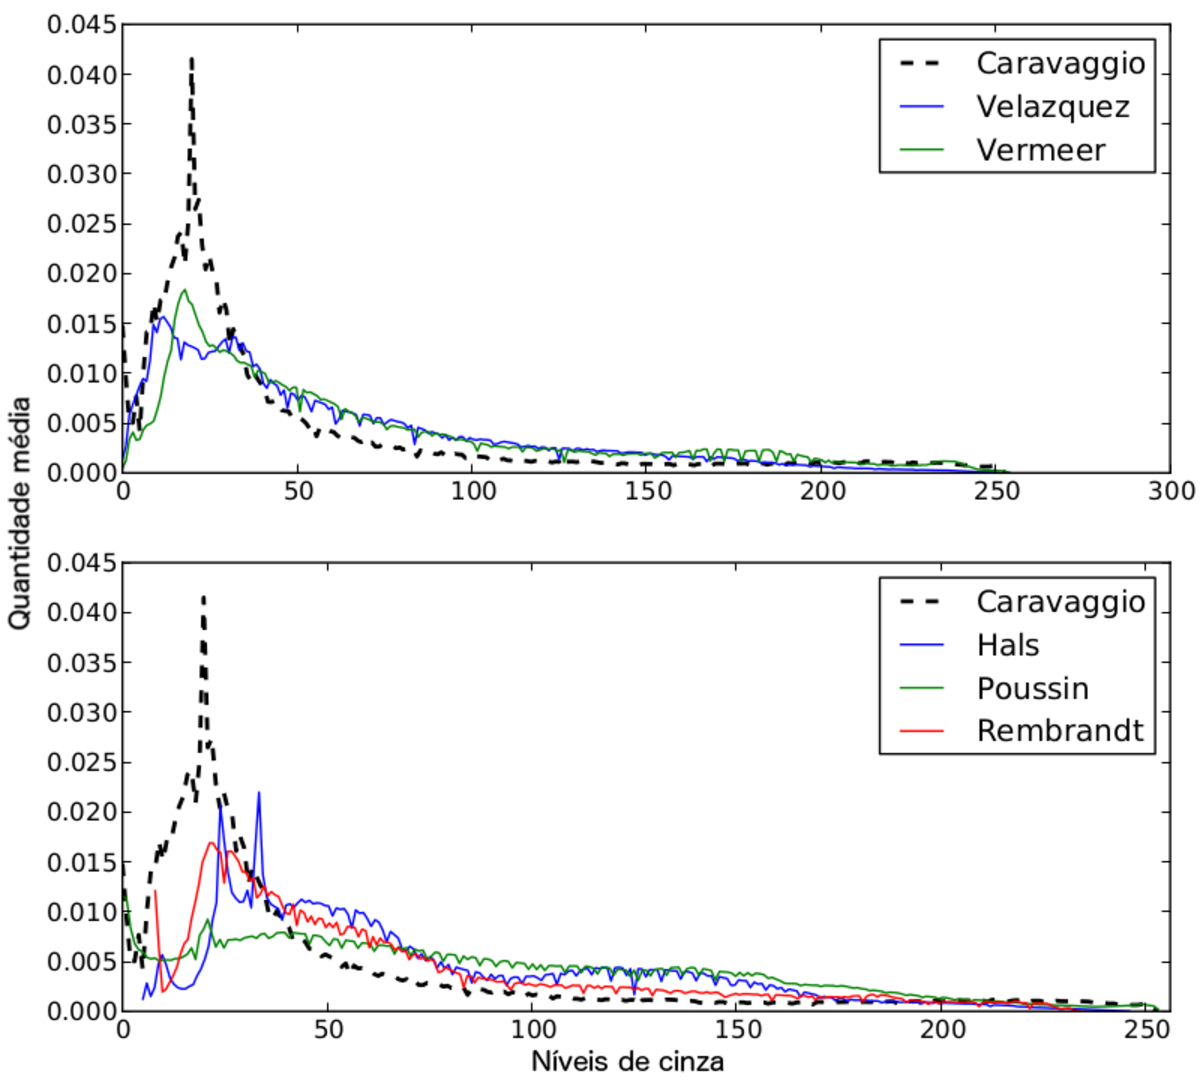
\includegraphics[width=.7\textwidth]{figs/chiaroscuro2}}
%       \caption{Histogramas dos níveis médios de cinza para todos os
%         pintores barrocos.} \label{fig:chiaroscuro}
%         \end{center}
% \end{figure}

% \end{frame}



\begin{frame}{Releitura do Barroco}
\setstretch{1.5}
\begin{columns}
 \begin{column}{.49\textwidth}
Caravaggio é expoente no uso da técnica do
  \textit{chiaroscuro}.

 \end{column}

 \begin{column}{.49\textwidth}

\begin{figure}[h!]
  \begin{center}
    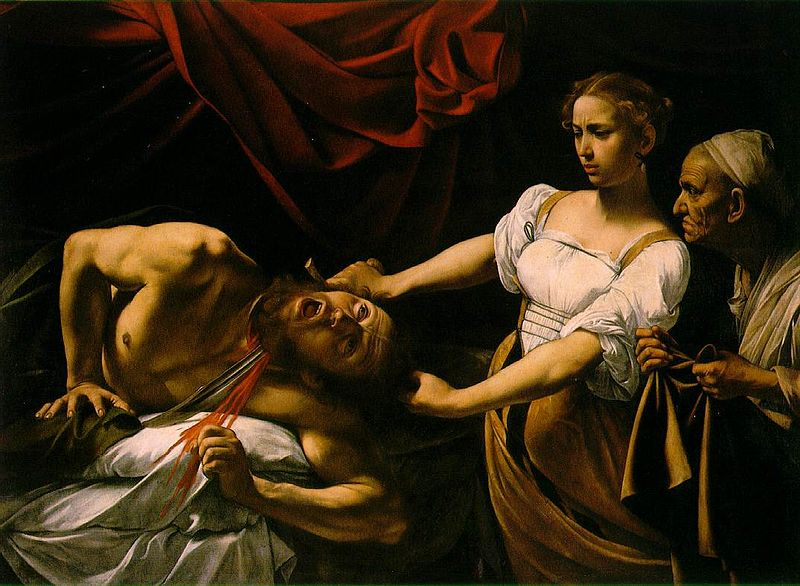
\includegraphics[width=1.0\textwidth]{figs/caravaggio_judite.png}
    \caption{\emph{Judite e Holoferne} (Caravaggio), c. 1599. \textit{Fonte: Wikipedia}.}
    \label{fig:caravaggio:judite}
\end{center}
\end{figure}

\end{column}
\end{columns}
\end{frame}

\begin{frame}{Releitura do Barroco}

  \begin{itemize}
    \item Influência de Caravaggio em
      pintores como Velázquez e Vermeer.

    \item Baixa similaridade entre histogramas de contrastes do período Barroco e Moderno.
    \end{itemize}

\end{frame}


\begin{frame}{Releitura do Barroco}

\begin{columns}
 \begin{column}{.4\textwidth}
  \begin{figure}[h!]
\begin{center}
  { \centering 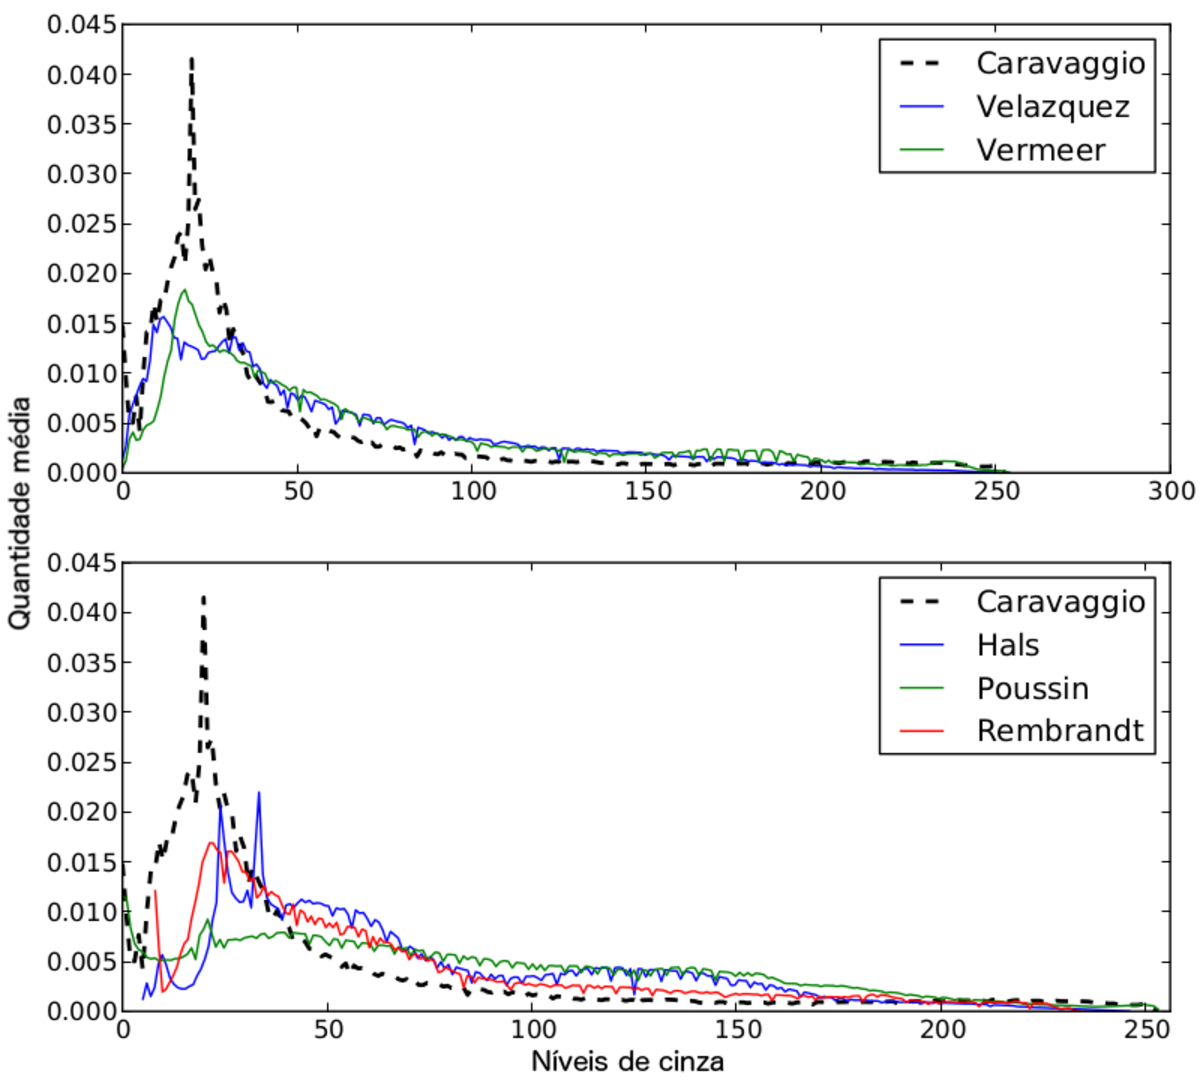
\includegraphics[width=\columnwidth]{figs/chiaroscuro2}}
      \caption{Barroco.} \label{fig:chiaroscuro}
        \end{center}
\end{figure}
 \end{column}

 \begin{column}{.6\textwidth}
 \begin{figure}[h!]
    
\begin{center}
{    \centering
        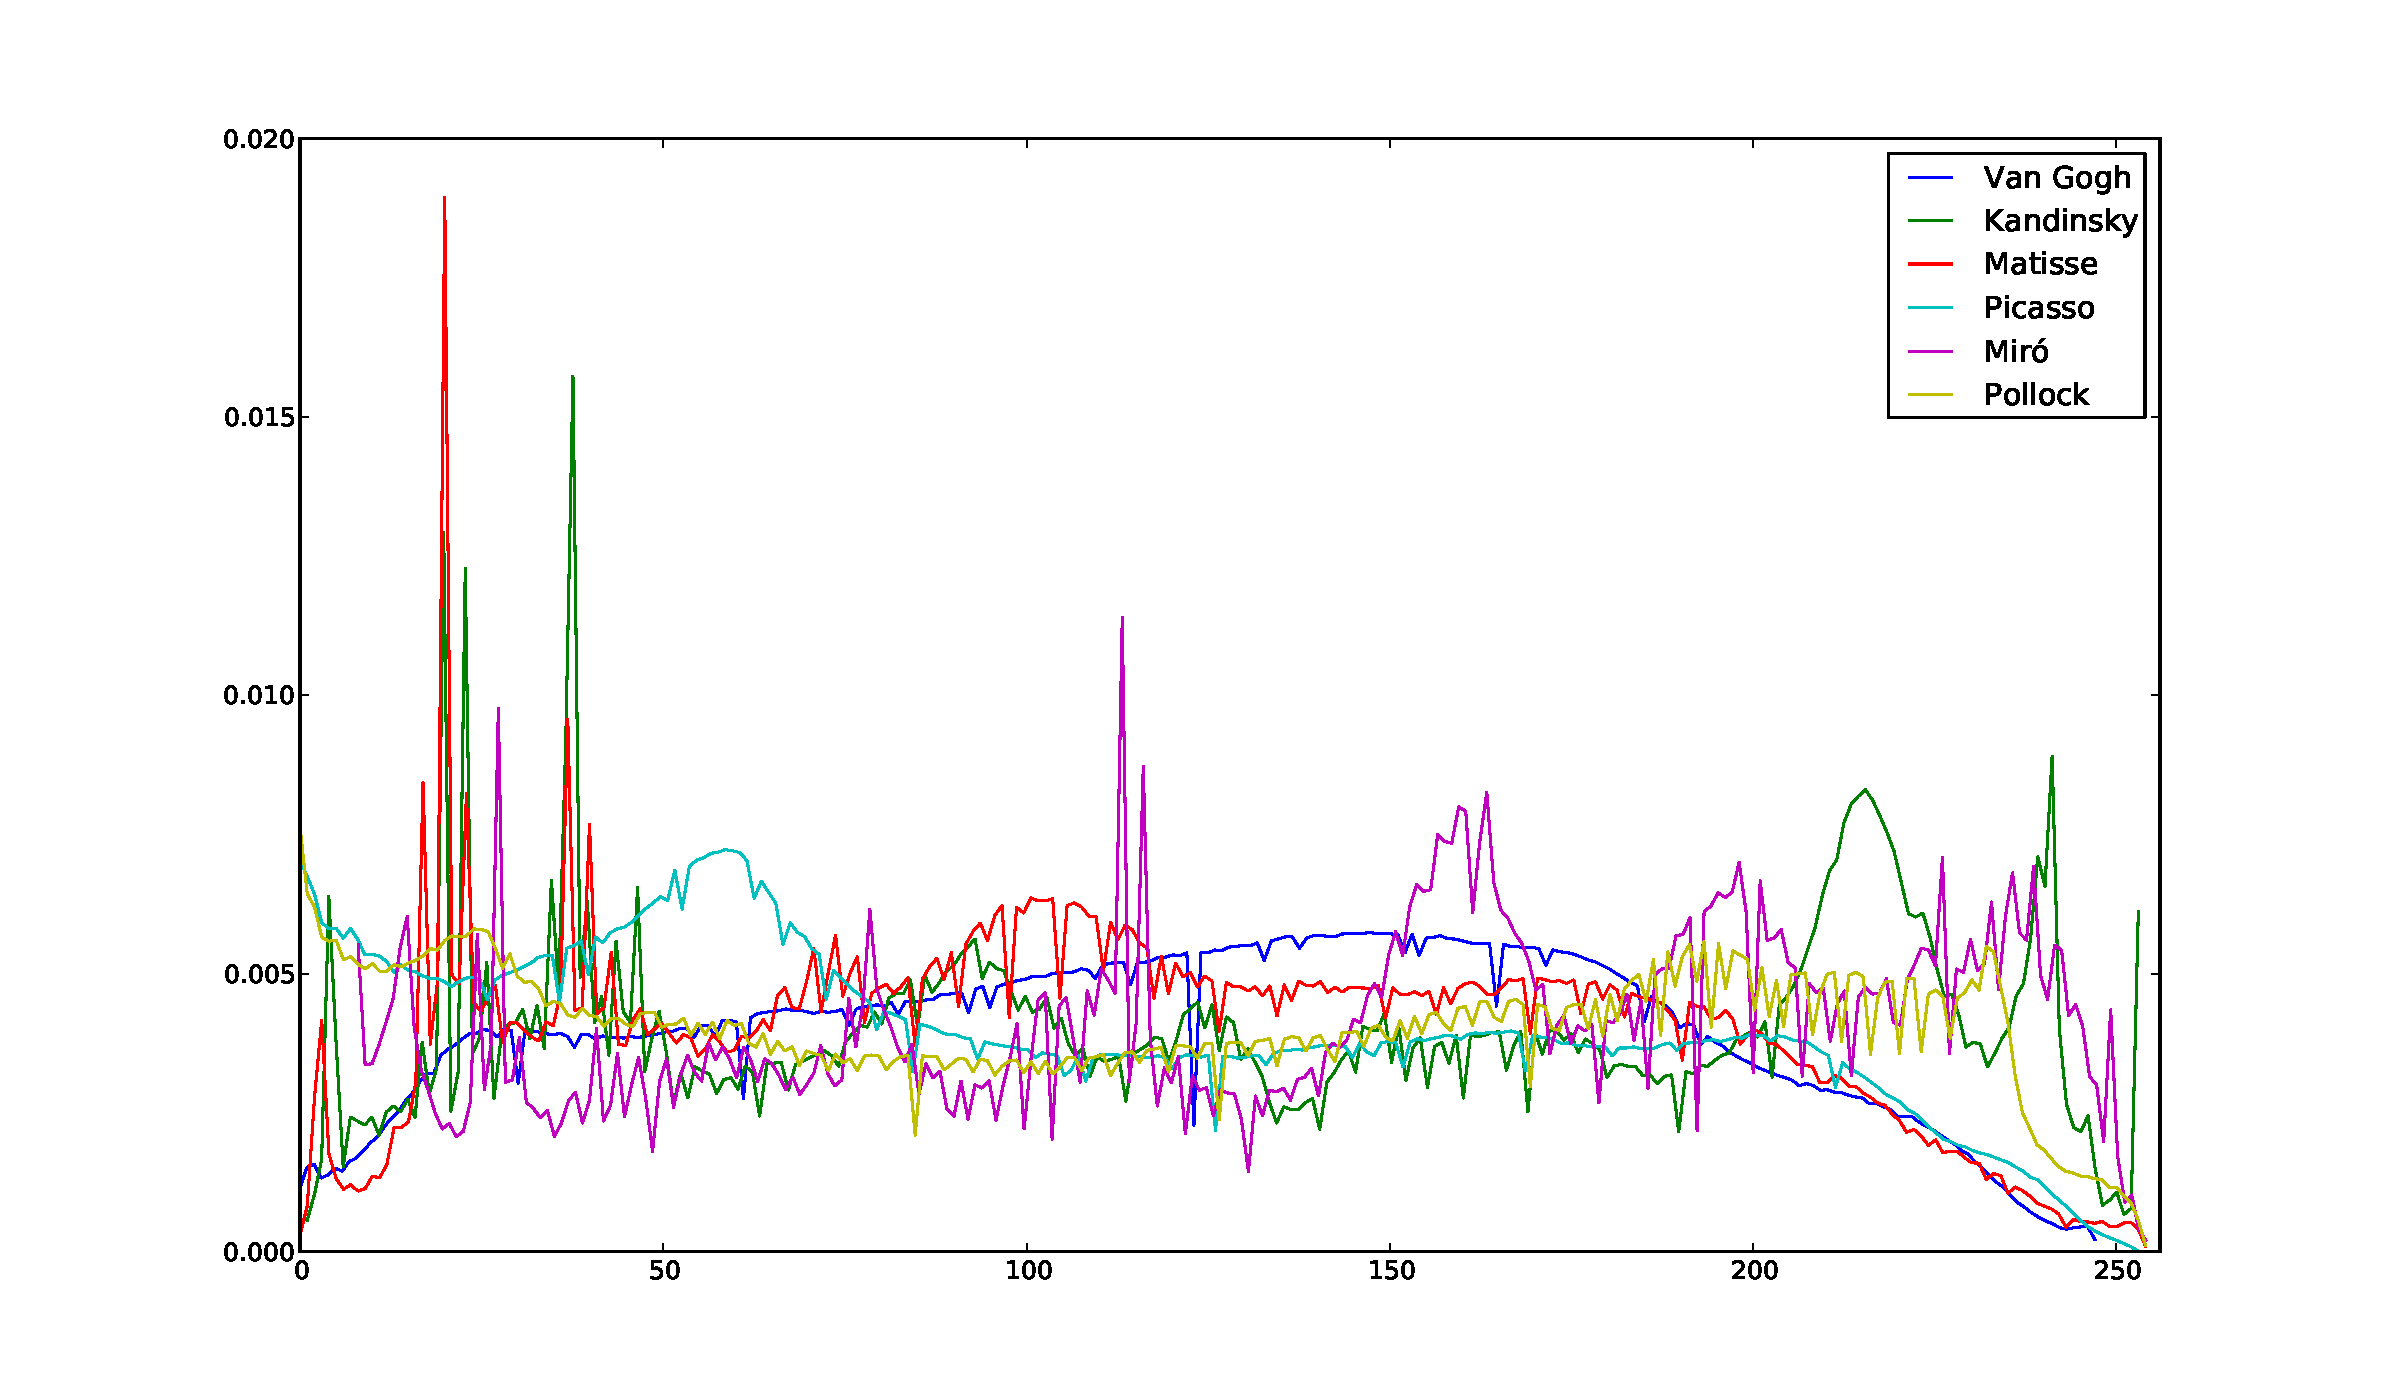
\includegraphics[width=\columnwidth]{figs/chiaroscuro_modernos}}
      \caption{Arte Moderna.}
        \label{fig:chiaroscuro_modernos}
  \end{center}
\end{figure}
  \end{column}
\end{columns}

\end{frame}



\begin{frame}{Releitura do Barroco}

Poussin se opõe à Caravaggio: ele não deseja retratar a verdade, 
mas sim o belo (influências de Carracci, Reni e Rafael).

\begin{figure}[h!]
  \begin{center}
    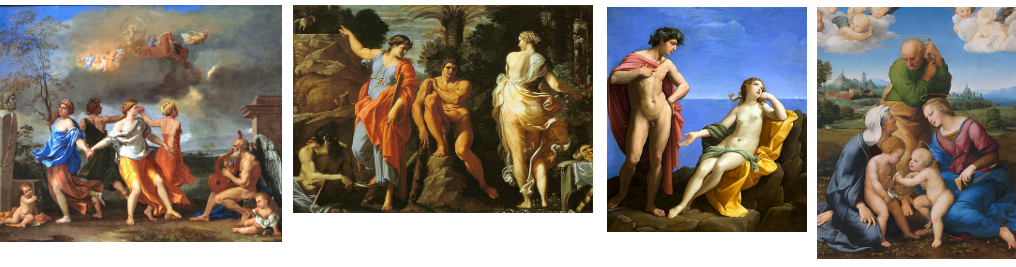
\includegraphics[width=1.0\textwidth]{figs/compara_poussin.png}
    \caption{Comparação entre pinturas de Poussin, Carracci, Reni e Rafael. \textit{Fonte: Wikipedia}.}
\end{center}
\end{figure}

\end{frame}

\begin{frame}{Releitura do Barroco}

\begin{columns}
 \begin{column}{.49\textwidth}
 \only<1>{
\begin{figure}[h!]
  \begin{center}
    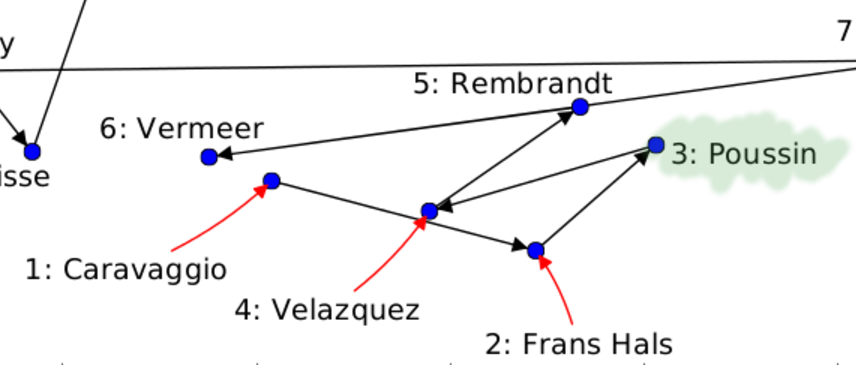
\includegraphics[width=1.2\columnwidth]{figs/caso1_g2_zoom3}
    \caption{Detalhe da série temporal.}
\end{center}
\end{figure}
}
 \only<2>{
\begin{figure}[h!]
  \begin{center}
    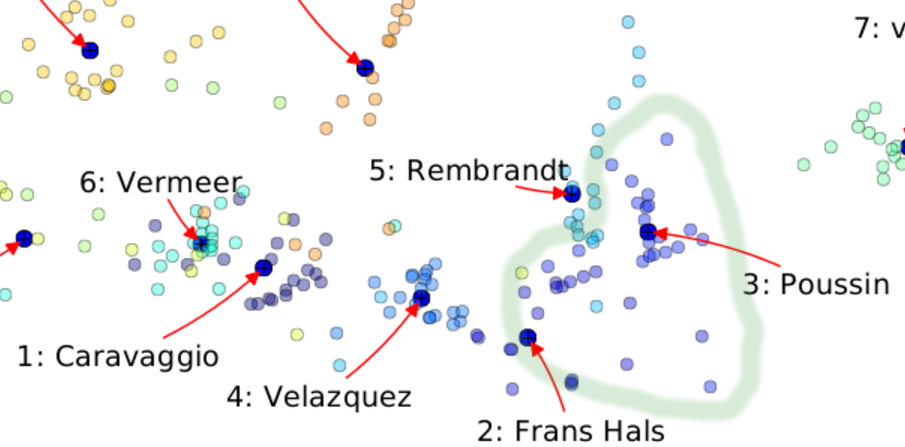
\includegraphics[width=1.2\columnwidth]{figs/caso1_g1_zoom3}
    \caption{Detalhe da projeção.}
\end{center}
\end{figure}
}
 \end{column}

 \begin{column}{.49\textwidth}
  \begin{itemize}
    \item<1>  É o pintor Barroco que mais se distancia de Caravaggio e do grupo Barroco.

    \item<2> Compreende o grupo de pinturas com
menor sobreposição.
  \end{itemize}
 \end{column}
\end{columns}

\end{frame}

% caso de estudo => movimentos da arte moderna



\subsection{Releitura da Arte Moderna}

\begin{frame}{Releitura da Arte Moderna}
  
  Pintores modernos são, em geral, independentes em estilo. Barrocos compartilham estilos
  tradicionais.

  \begin{figure}[h!]
  \begin{center}
    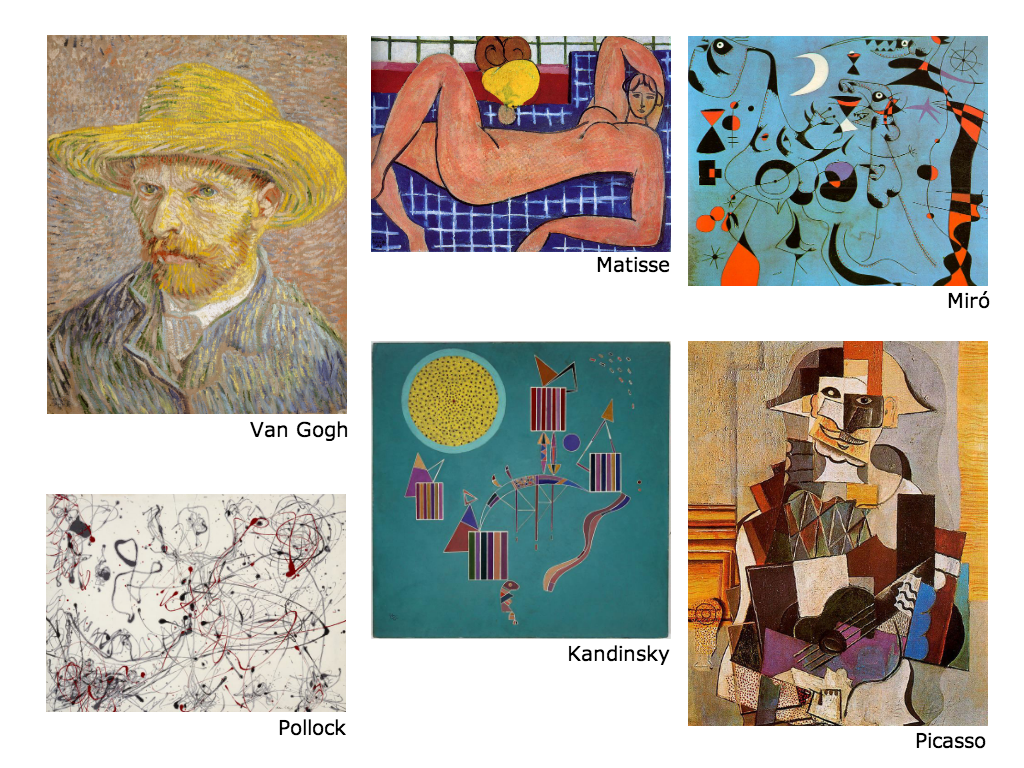
\includegraphics[width=0.65\textwidth]{figs/compara_moderno2.png}
    \caption{Comparação entre pinturas modernas. \textit{Fonte: Wikipedia}.}
\end{center}
\end{figure}

\end{frame}

\begin{frame}{Releitura da Arte Moderna}

\begin{columns}
 \begin{column}{.49\textwidth}
 \only<1>{
\begin{figure}[h!]
  \begin{center}
    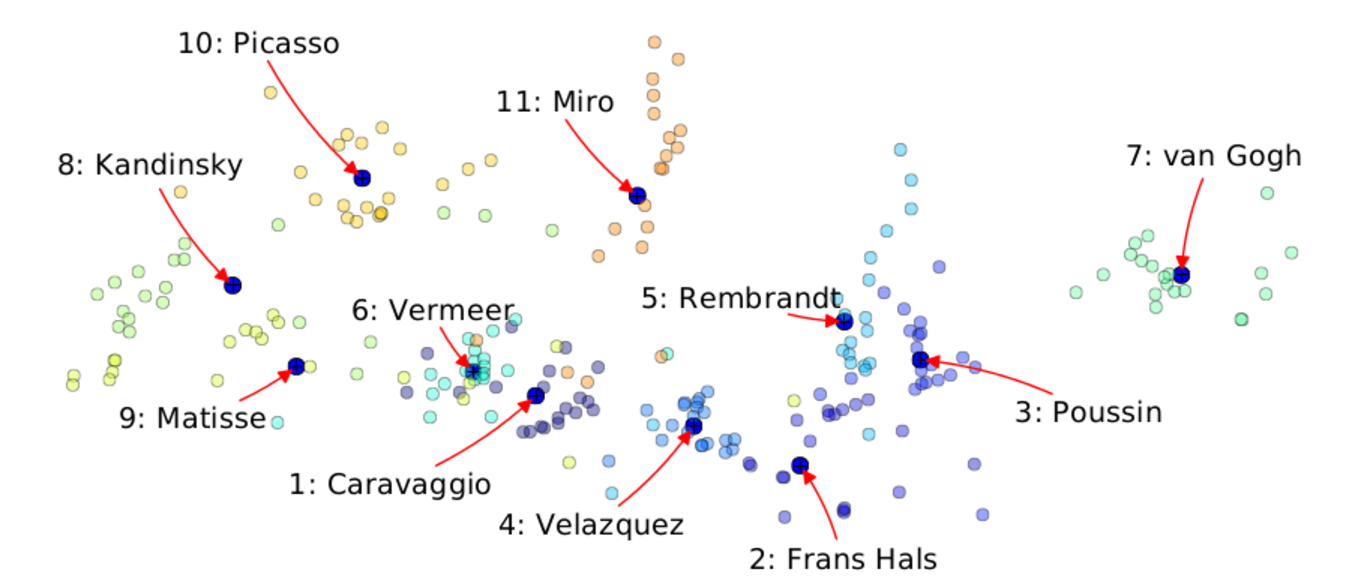
\includegraphics[width=1.2\columnwidth]{figs/caso1_g1_zoom1}
    \caption{Detalhe da série temporal.}
\end{center}
\end{figure}
}
 \only<2>{
\begin{figure}[h!]
  \begin{center}
    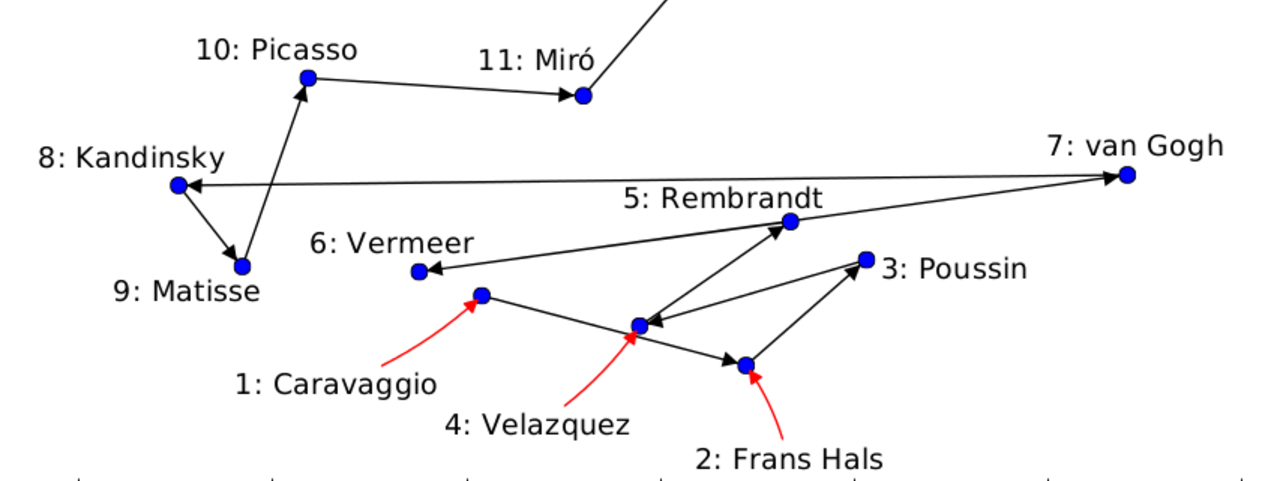
\includegraphics[width=1.2\columnwidth]{figs/caso1_g2_zoom1}
    \caption{Detalhe da projeção.}
\end{center}
\end{figure}
}
 \end{column}

 \begin{column}{.49\textwidth}
  \begin{itemize}
    \item<1> Há maior sobreposição entre pintores barrocos do que modernos.

    \item<2> Os deslocamentos entre pintores modernos são, em geral, maiores.

    \item<2> Maior exploração do espaço por parte dos artistas modernos.
  \end{itemize}
 \end{column}
\end{columns}

\end{frame}



% \begin{frame}{Releitura da Arte Moderna}

%   Diferença cronológica e estética entre o Barroco
%   e os movimentos da Arte Moderna.

%   \begin{figure}[h!]
%   \begin{center}
%     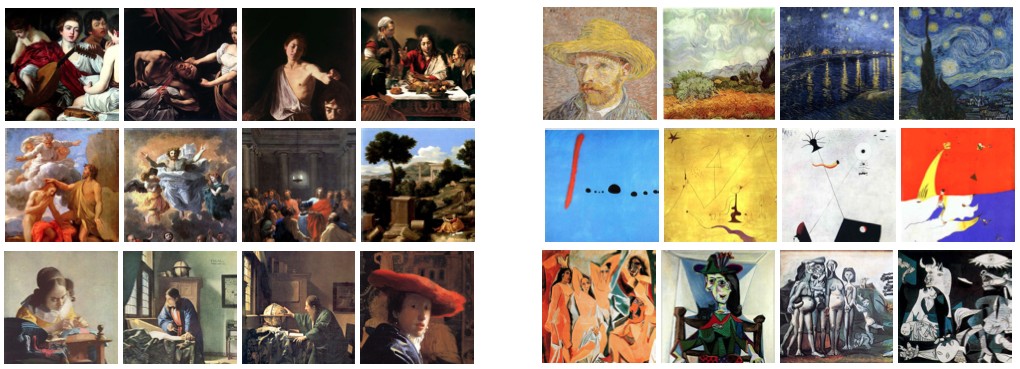
\includegraphics[width=1.0\textwidth]{figs/compara_bar_mod.png}
%     \caption{Comparação entre pinturas barrocas e modernas.}
% \end{center}
% \end{figure}

% \end{frame}

% \begin{frame}{Releitura da Arte Moderna}

% \begin{columns}
%  \begin{column}{.49\textwidth}
% \begin{figure}[h!]
%   \begin{center}
%     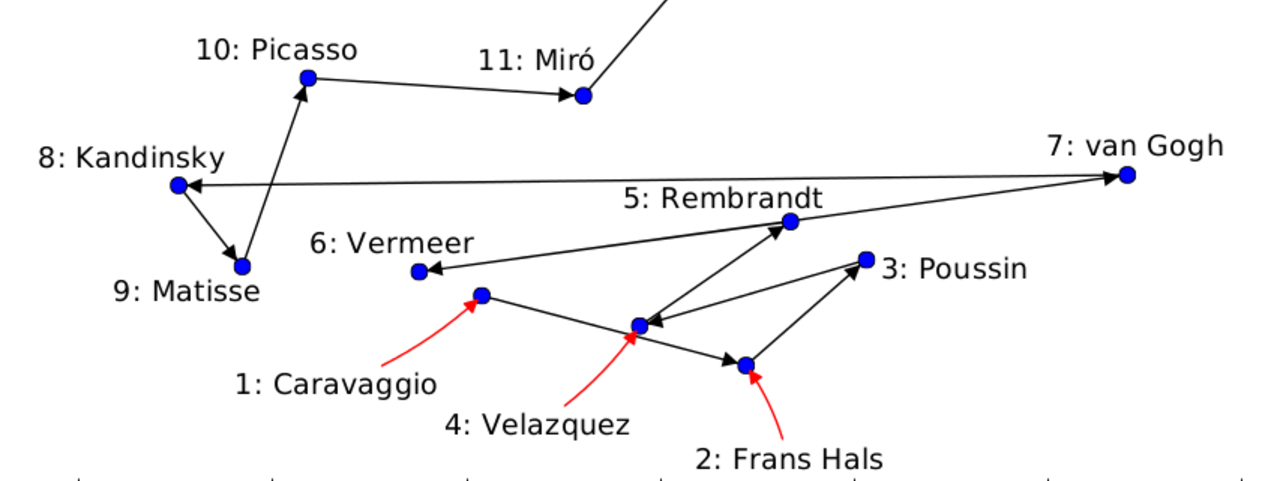
\includegraphics[width=1.2\columnwidth]{figs/caso1_g2_zoom1}
%     \caption{Detalhe da projeção.}
% \end{center}
% \end{figure}
%  \end{column}

%  \begin{column}{.49\textwidth}
%   \begin{itemize}
%     \item Os barrocos retornam uns aos outros.

%     \item Há deslocamento abrupto em Van Gogh.
%   \end{itemize}
%  \end{column}
% \end{columns}

% \end{frame}

%%%%%%
%%%%%%
%%%%%%

\begin{frame}{Releitura da Arte Moderna}

  Pollock apresenta pinturas que diferem de todos os outros
  pintores escolhidos.

  \begin{figure}[h!]
  \begin{center}
  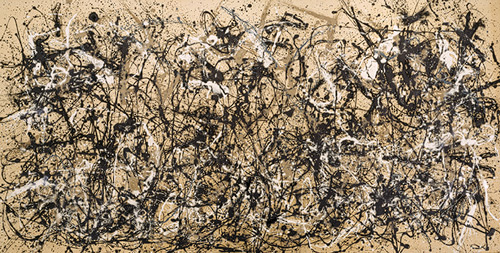
\includegraphics[width=0.9\textwidth]{figs/pollock_ritmo.png}
  \caption{\emph{Ritmo de Outono} (Jackson Pollock), c. 1950. \textit{Fonte: Wikipedia}.}
  \label{fig:pollock:ritmo}
  \end{center}
\end{figure}

\end{frame}

\begin{frame}{Releitura da Arte Moderna}

\begin{columns}
 \begin{column}{.49\textwidth}
\begin{figure}[h!]
  \begin{center}
    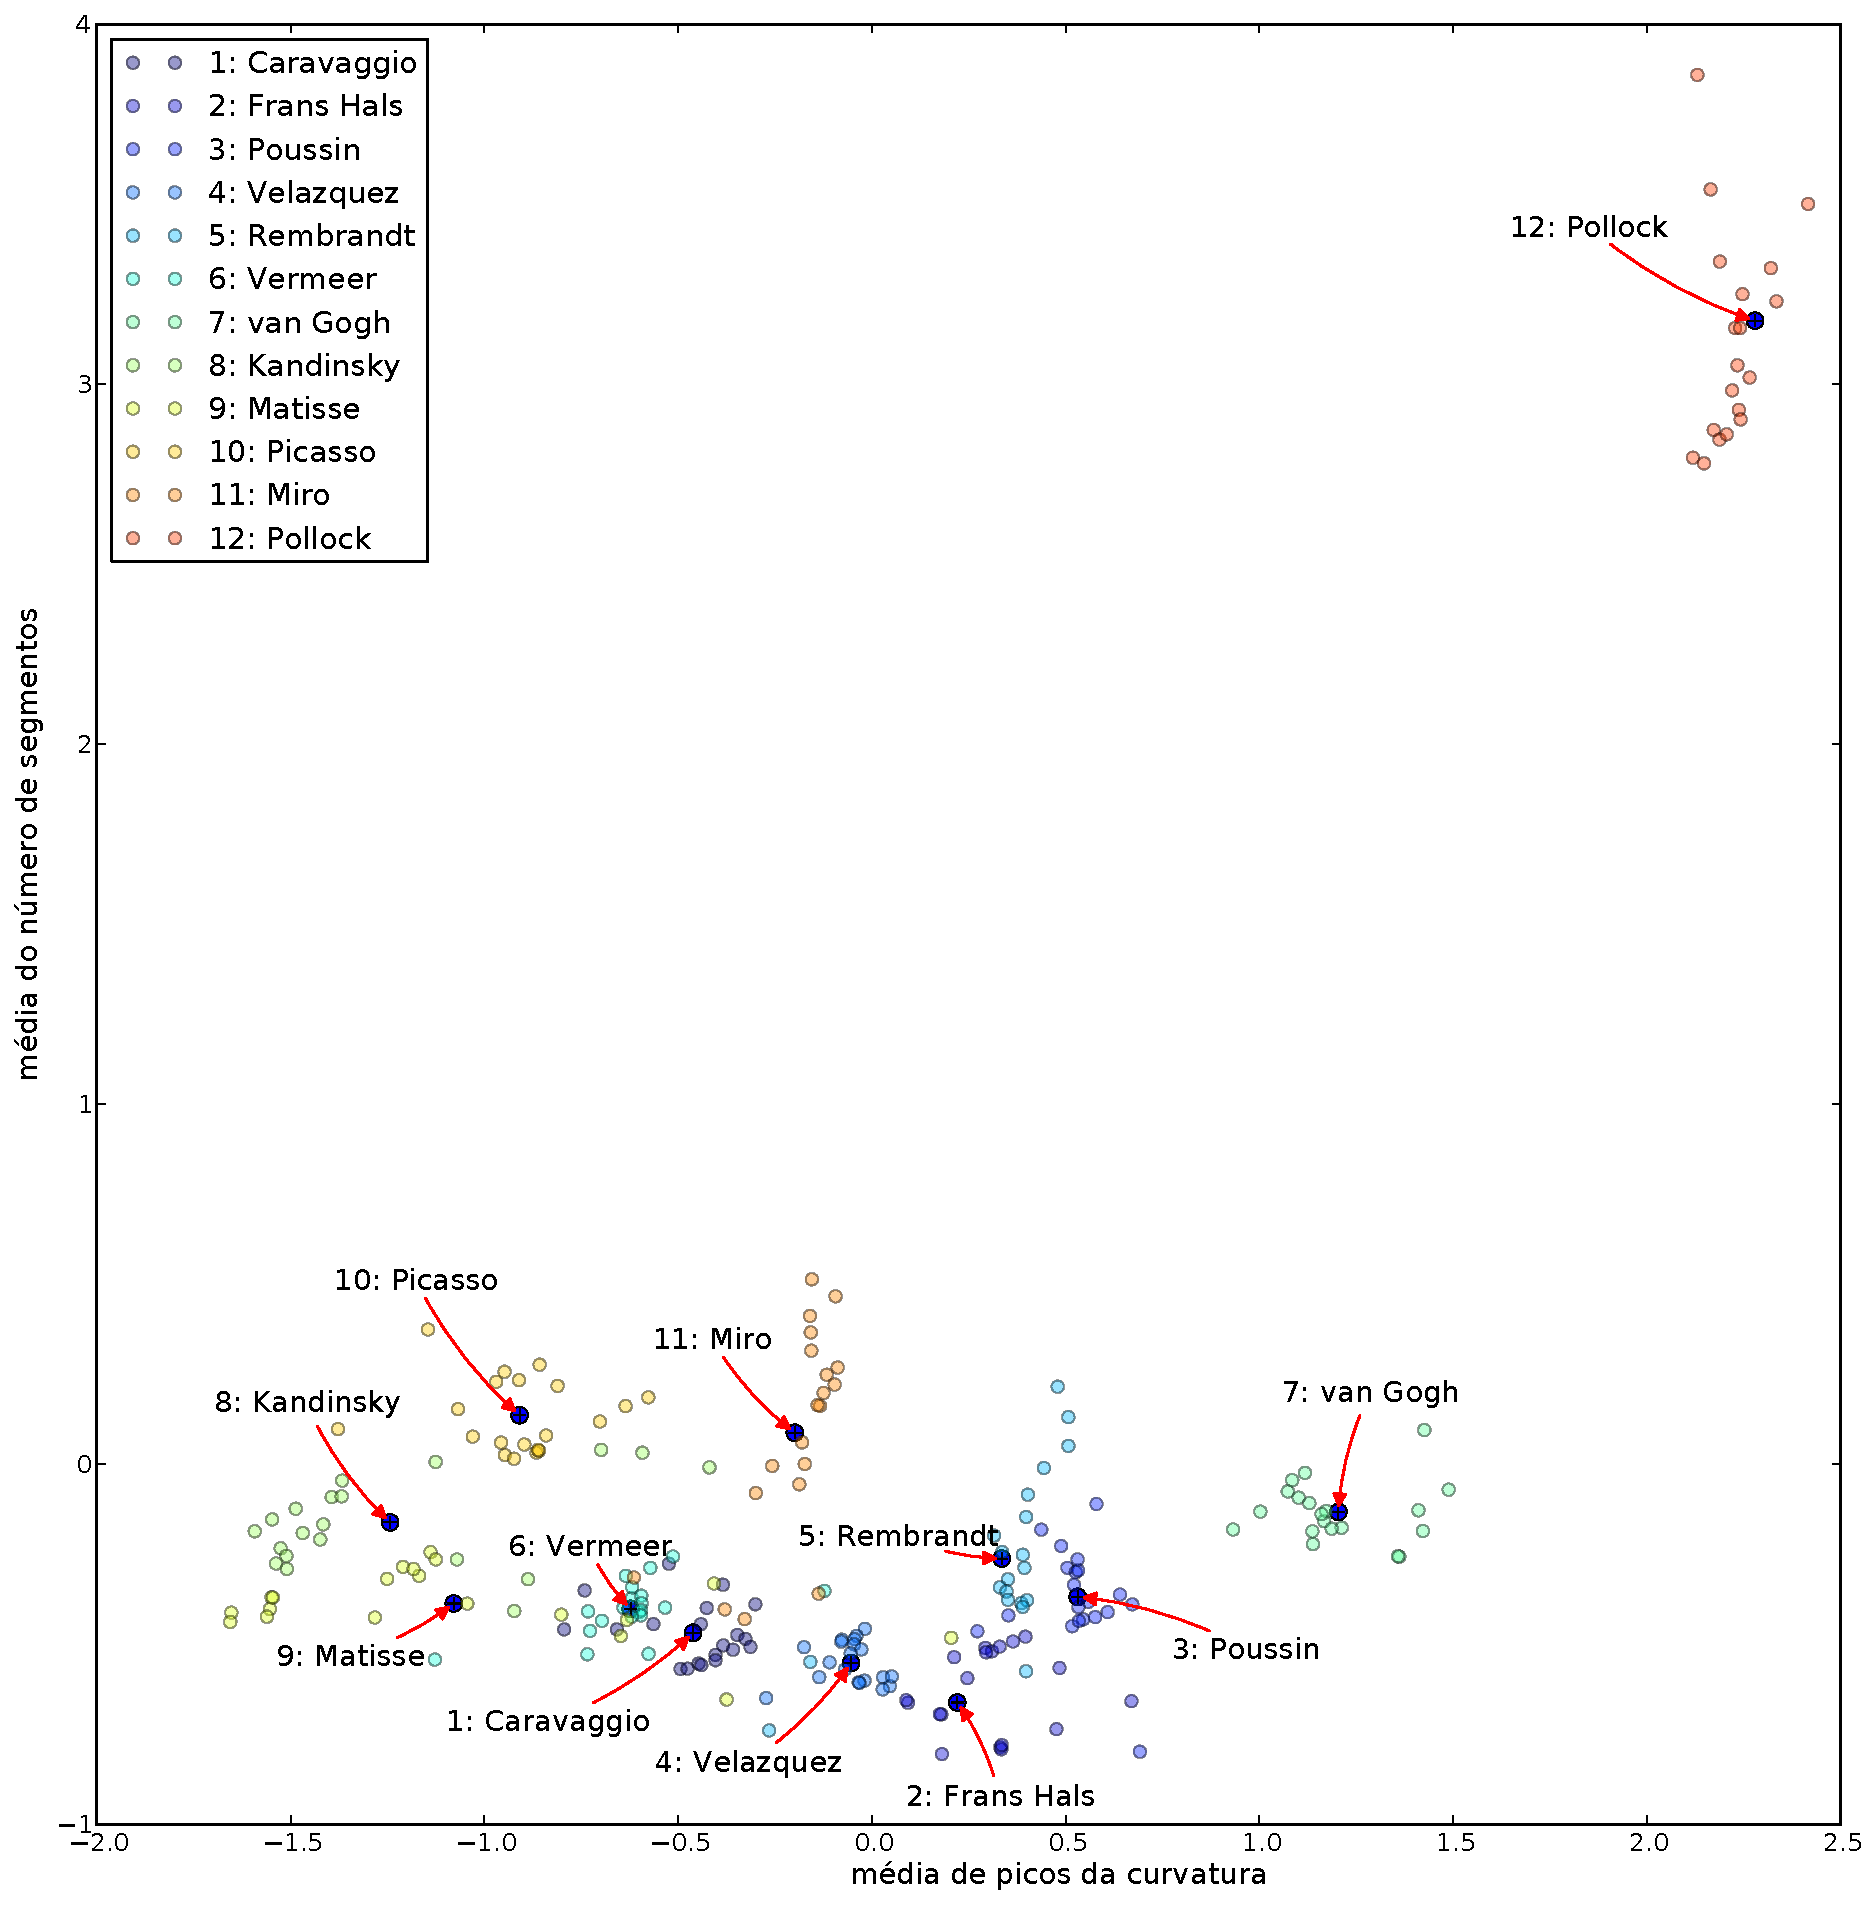
\includegraphics[width=\columnwidth]{figs/caso1_g1}
    \caption{Detalhe da projeção.}
\end{center}
\end{figure}
 \end{column}

 \begin{column}{.49\textwidth}
  \begin{itemize}
    \item O ``cluster'' de Pollock é o que mais se distancia dos demais.

    \item Principalmente considerando-se o eixo-$y$ (média do número de segmentos).
  \end{itemize}
 \end{column}
\end{columns}

\end{frame}


%%%%

\begin{frame}{Medidas de oposição, inovação e dialética}

\begin{figure}[ht!]
\begin{center}
% \caption{\textit{a)} \textit{Dialética}: um argumento chamado \textit{tese}, até então
%   tomado como verdade, é confrontado por um argumento oposto,
%   chamado \textit{antítese}. O resultado do confronto destas duas
%   ideias é a \textit{síntese} que poderá gerar uma nova ideia ou
%   argumento; \textit{b)} \textit{Oposição}: é um argumento que se opõe
%   a um argumento original; \textit{c)} \textit{Inovação}: um movimento
%   de inovação é aquele que se afasta do argumento original, inovando.}
% \label{fig:conceitos}

\begin{tikzpicture}[scale=.8]
  % Dialética
  \node[draw] (Tese) at (0,0) {Tese};
  \node[draw,fill=black,text=white] (Antitese) at (2.3,0) {Antítese};
  \node[draw,fill=gray,text=white] (Sintese) at (1,2) {Síntese};
  
  \draw node[vertex] (Juncao) at (1,0) {};
  
  \draw[-,draw=blue] (Tese) to (Juncao);
  \draw[->,draw=blue] (Juncao) to (Antitese);
  \draw[->,draw=blue] (Juncao) to (Sintese);
  %\draw[->,draw=blue] (Sintese) to[in=180,out=180] (Tese);
  
  \node at (1.0, -1.0) {\textit{a) Dialética}};
  
  % Oposição
  \node[draw] (ArgumentoA) at (5,0) {Argumento};
  \node[draw,fill=black,text=white] (ArgumentoB) at (7.5,0) {Oposição};
  
  \draw[->,draw=blue] (ArgumentoA) to (ArgumentoB);
  
  \node at (6., -1.0) {\textit{b) Oposição}};
  
  % Inovação
  \node[draw] (ArgumentoA) at (10.1,0) {Argumento};
  %\node[draw,fill=black,text=white] (ArgumentoB) at (12.8,0) {Oposição};
  \node[draw,fill=yellow] (ArgumentoC) at (12,2) {Inovação};
  
  %\draw node[vertex] (Juncao) at (11.5,0) {};
  
  %\draw[-] (ArgumentoA) to (Juncao);
  %\draw[->] (Juncao) to (ArgumentoB);
  \draw[->,draw=blue] (ArgumentoA) to (ArgumentoC);
  
  \node at (11.5, -1.0) {\textit{c) Inovação}};

\end{tikzpicture}
\caption{Representação em diagrama para conceitos da Filosofia.}
\end{center}
\end{figure}

\end{frame}

% \begin{frame}{Como medidas}

%   \begin{itemize}
%   \item Define-se um espaço $N_f$-dimensional a partir dos $N_f$ vetores de atributos $\vec{f_i}$
%   \item Esse espaço é chamado de \textit{espaço criativo} ou \textit{espaço de pinturas}
%   \item Cada pintura $\vec{f_i} \in C_p$, sendo $C_p$ uma classe de pinturas ou um pintor
%   \item Define-se um protótipo $\vec{p_i}$ para cada classe $C_p$
%   \item O protótipo $\vec{p_i}$ equivale ao centróide das pinturas de uma classe
%   \begin{equation}
%     \vec{p_i} = \frac{1}{N_p} \sum_{i=1}^{N_p} \vec{f_i}
%   \end{equation}
%   \end{itemize}
% \end{frame}

% \begin{frame}{O método quantitativo}

%   \begin{itemize}
%     \item $S$ define uma série temporal de $\vec{p_i}$ estados, modelando o que seria a linha cronológica das pinturas
%     \item $\vec{a}_i$: estado médio em dado tempo $i$ abrangendo os estados $\vec{p_1}$ até $\vec{p_i}$
%     \begin{equation}
%       \vec{a}_i = \frac{1}{i}\sum_{j=1}^i\vec{p}_j
%     \end{equation}
%     \item $\vec{r}_i$: medida de oposição à $\vec{p_i}$
%     \begin{equation}
%       \vec{r}_i = \vec{p}_i + 2(\vec{a}_i - \vec{p}_i)
%     \end{equation}
%     \item $\vec{D}_i$: vetor de oposição, representando o deslocamento do estado $\vec{r}_i$ em relação a $\vec{p}_i$
%     \begin{equation}
%       \vec{D}_i=\vec{r}_i - \vec{p}_i
%     \end{equation}
%     \item $\vec{M}_{i,j}$: deslocamento de um estado $\vec{p}_i$ até outro estado a $\vec{p}_j$
%     \begin{equation}
%     \vec{M}_{i,j} = \vec{p}_j - \vec{p}_i
%     \end{equation}

%   \end{itemize}

% \end{frame}

% \begin{frame}{Medidas de oposição, inovação e dialética}

%   \begin{itemize}
%     \item Índice de oposição $W_{i,j}$ entre $\vec{p}_i$ e $\vec{p}_j$
%     \begin{equation}
%     W_{i,j} = \frac{\left< \vec{M}_{i,j}, \vec{D}_i\right>}{||\vec{D}_i||^2}
%     \end{equation}
%     \item Índice de inovação $s_{i,j}$
%     \begin{equation}
%     s_{i,j} = \sqrt{\frac{|\vec{p}_i-\vec{p}_j|^2
%           |\vec{a}_i-\vec{p}_i|^2 - 
%           [(\vec{p}_i-\vec{p}_j) . 
%             (\vec{a}_i-\vec{p}_i)]^2}
%         {|\vec{a}_i-\vec{p}_i|^2}}
%     \end{equation}
%     \item Índice de contra-dialética $d_{i}$ entre tese, antítese e síntese
%     \begin{equation}
%     d_{i \rightarrow k} = 
%       \frac{|\left< \vec{p}_j-\vec{p}_i,\vec{p}_k \right> + 
%         \frac{1}{2}\left<\vec{p}_i-\vec{p}_j, \vec{p}_i+\vec{p}_j\right>|}
%            {|\vec{p}_j-\vec{p}_i|}
%     \end{equation}
%   \end{itemize}

% \end{frame}

\begin{frame}{Medidas de oposição e inovação}

% \begin{columns}
%  \begin{column}{.49\textwidth}
%  \begin{itemize}
%   \item<1> $S$: série temporal de $\vec{p}_i$ estados
%   \item<2> $\vec{a}_i$: estado médio em dado tempo $i$ abrangendo os estados $\vec{p_1}$ até $\vec{p_i}$
%   \item<3> $\vec{r}_i$: medida de oposição à $\vec{p_i}$
%   \item<4> $\vec{D}_i$: vetor de oposição, representando o deslocamento do estado $\vec{r}_i$ em relação a $\vec{p}_i$
%   \item<5> $W_{i,j}$: índice de oposição
%   \item<6> $s_{i,j}$: índice de inovação
%  \end{itemize}
%  \end{column}

%  \begin{column}{.49\textwidth}
\begin{figure}[ht!]
\begin{center}
        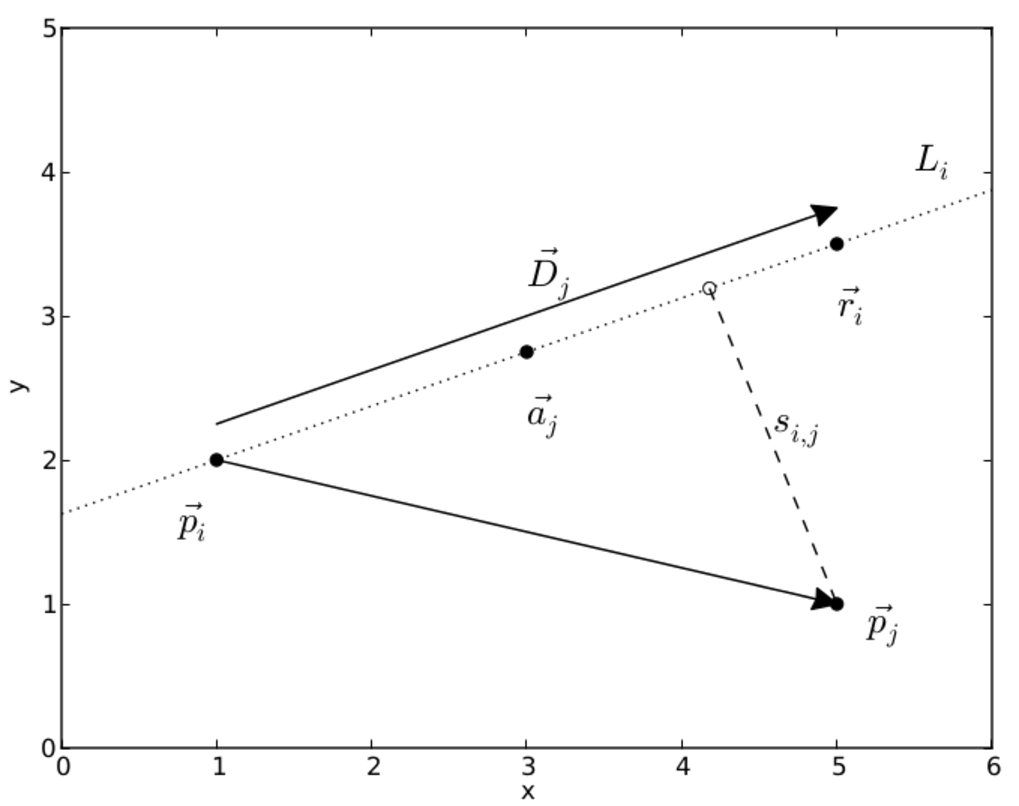
\includegraphics[width=.7\textwidth]{figs/desc_opos2.pdf}
              \caption{Exemplo de cálculo de $W_{i,j}$ e $s_{i,j}$.}
        \label{fig:desc_opos_inov}
\end{center}
\end{figure}
% \end{column}
% \end{columns}
\end{frame}

\begin{frame}{Medida de dialética}

% LEGENDAR ESTADOS

% \begin{columns}
%  \begin{column}{.49\textwidth}
%  \begin{itemize}
%   \item<1> $\vec{p_i}$: tese
%   \item<1> $\vec{p_j}$: antítese
%   \item<1> $\vec{p_k}$: síntese
%   \item<2> $B_{i,j}$: mediatriz entre $\vec{p_i}$ e $\vec{p_j}$
%   \item<3> $d_{i \rightarrow k}$: índice de contra-dialética
% \end{itemize}
% \end{column}
%  \begin{column}{.49\textwidth}
\begin{figure}[ht!]
\begin{center}
      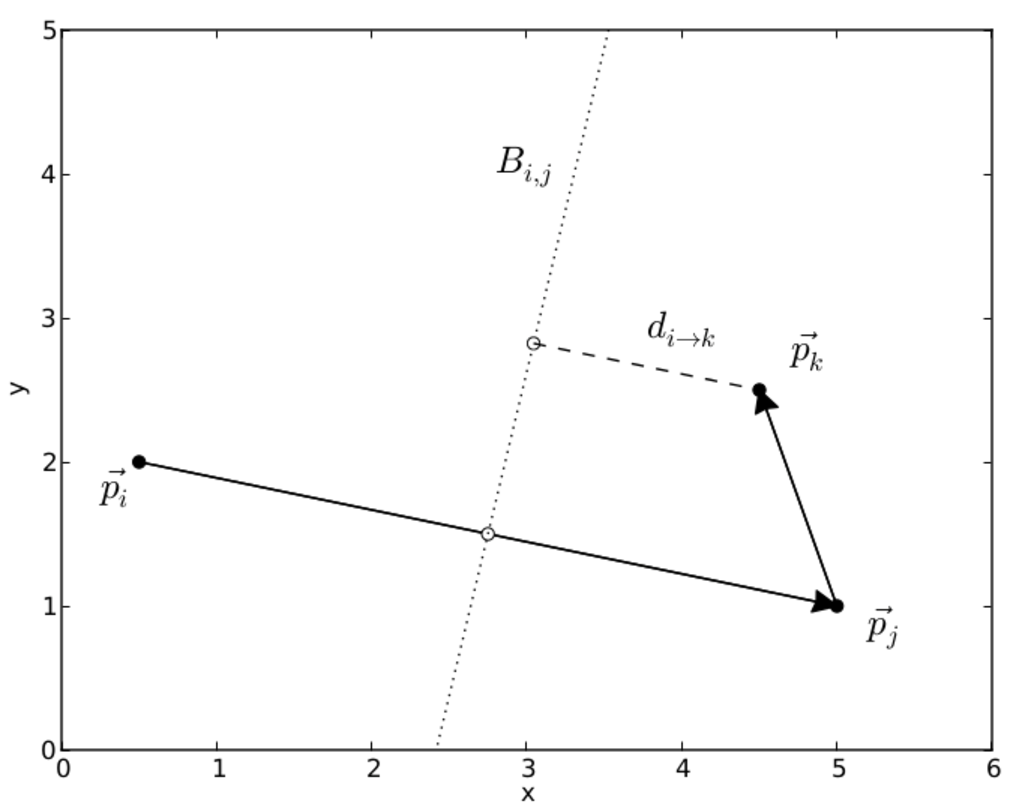
\includegraphics[width=.7\textwidth]{figs/desc_dialetica2.pdf}
      \caption{Exemplo de cálculo de $d_{i \rightarrow k}$.}
        \label{fig:desc_dialetica}
\end{center}
\end{figure}
% \end{column}
% \end{columns}
\end{frame}

\begin{frame}{Interpretação das medidas de oposição e inovação}
  \begin{figure}[h!]
\begin{center}
        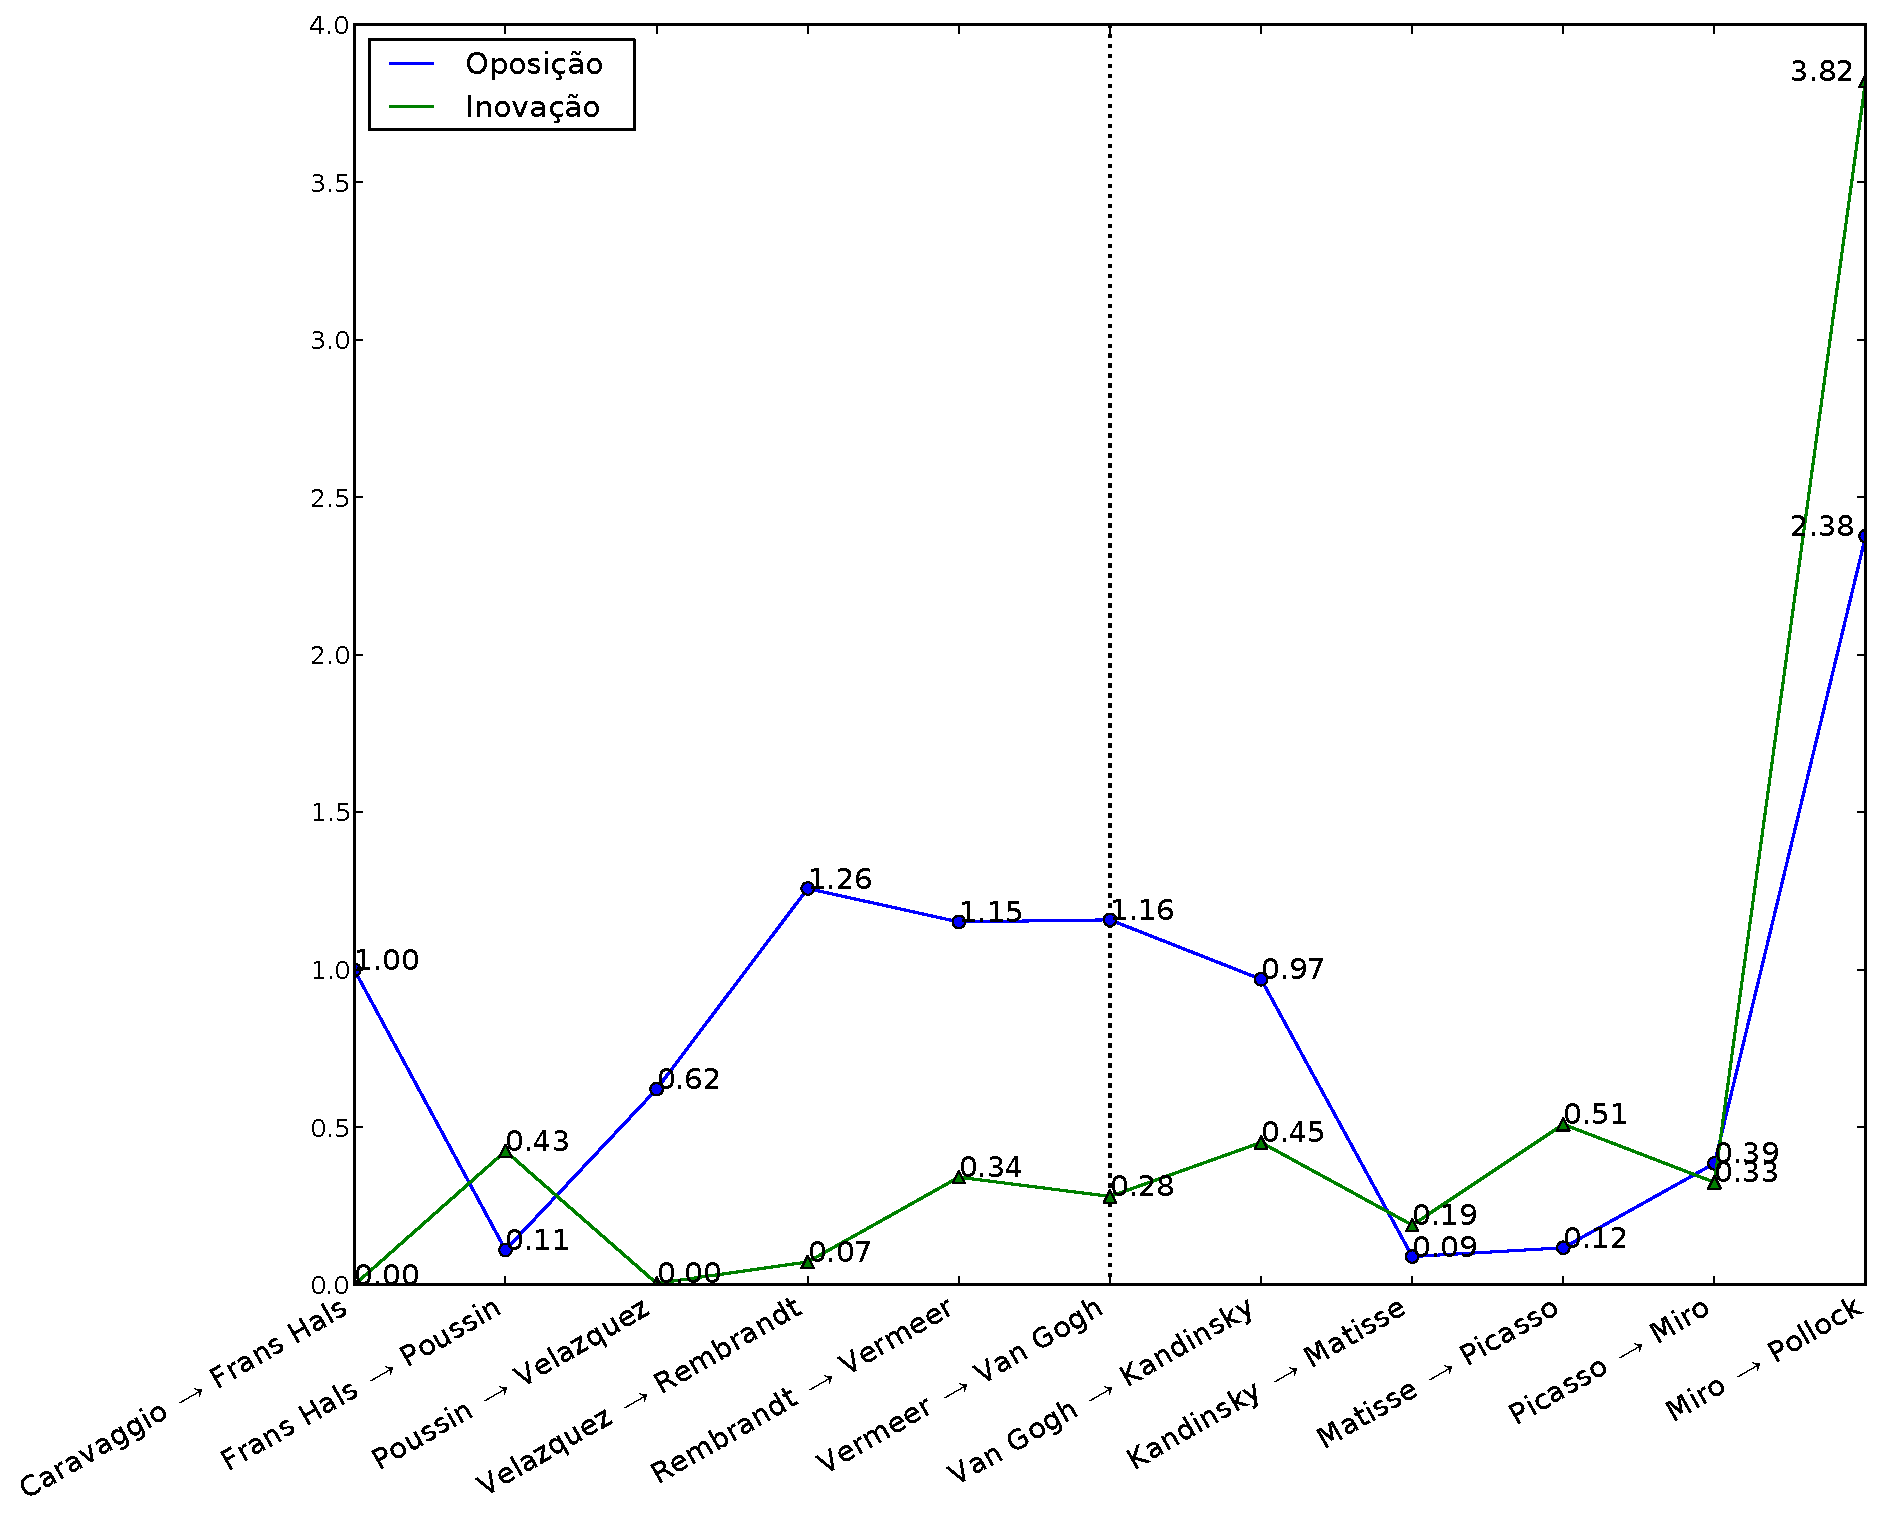
\includegraphics[width=.7\textwidth]{figs/caso1_oposEinov}
         \caption{Valores de $W_{i,j}$ e $s_{i,j}$ considerando
        os dois melhores atributos.}
        \label{fig:caso1_oposEinov}
\end{center}
\end{figure}
\end{frame}

\begin{frame}{Interpretação das medidas de oposição e inovação}
\setstretch{1.5}
      \begin{itemize}

  \item<1> Embora oscilante, a inovação é crescente.

  \item<2> Grande oposição entre Vermeer e Van Gogh.
  \item<2> $\to$ Quando há a transição do Barroco para o Moderno.

  \item<3> Maiores valores de oposição e inovação em Pollock.
  \item<3> $\to$ Pollock é o pintor que mais se diferencia de todos os demais.

  \item<4> Maior oposição está entre Velázquez e Rembrandt.
  \item<4> $\to$ Pinturas de Rembrandt nada têm de parecido com as de Velázquez.

 % \item<5> Grande inovação entre Van Gogh e Kandinsky.
 %  \item<5> $\to$ Obras de Kandinsky são abstratas, comparadas às de Van Gogh.

 %  \item<6> Maior inovação da Arte Moderna está entre Matisse e Picasso.
 %  \item<6> $\to$ Início do Cubismo.
  

    \end{itemize}
 \end{frame}

% \begin{frame}{Interpretação das medidas de oposição e inovação}

%       \begin{itemize}

%   \item<1> Grande inovação entre Van Gogh e Kandinsky.
%   \item<1> $\to$ Obras de Kandinsky são abstratas, comparadas às de Van Gogh.

%   \item<2> Maior inovação da Arte Moderna está entre Matisse e Picasso.
%   \item<2> $\to$ Início do Cubismo.

%   % \item<3> Baixa oposição entre Matisse e Picasso.
%   % \item<3> $\to$ Ambos retratavam formas humanas com preferência por linhas retas.

%     \end{itemize}

% \end{frame}

\begin{frame}{Interpretação das medidas de dialética}
  \begin{figure}[h!]
\begin{center}
        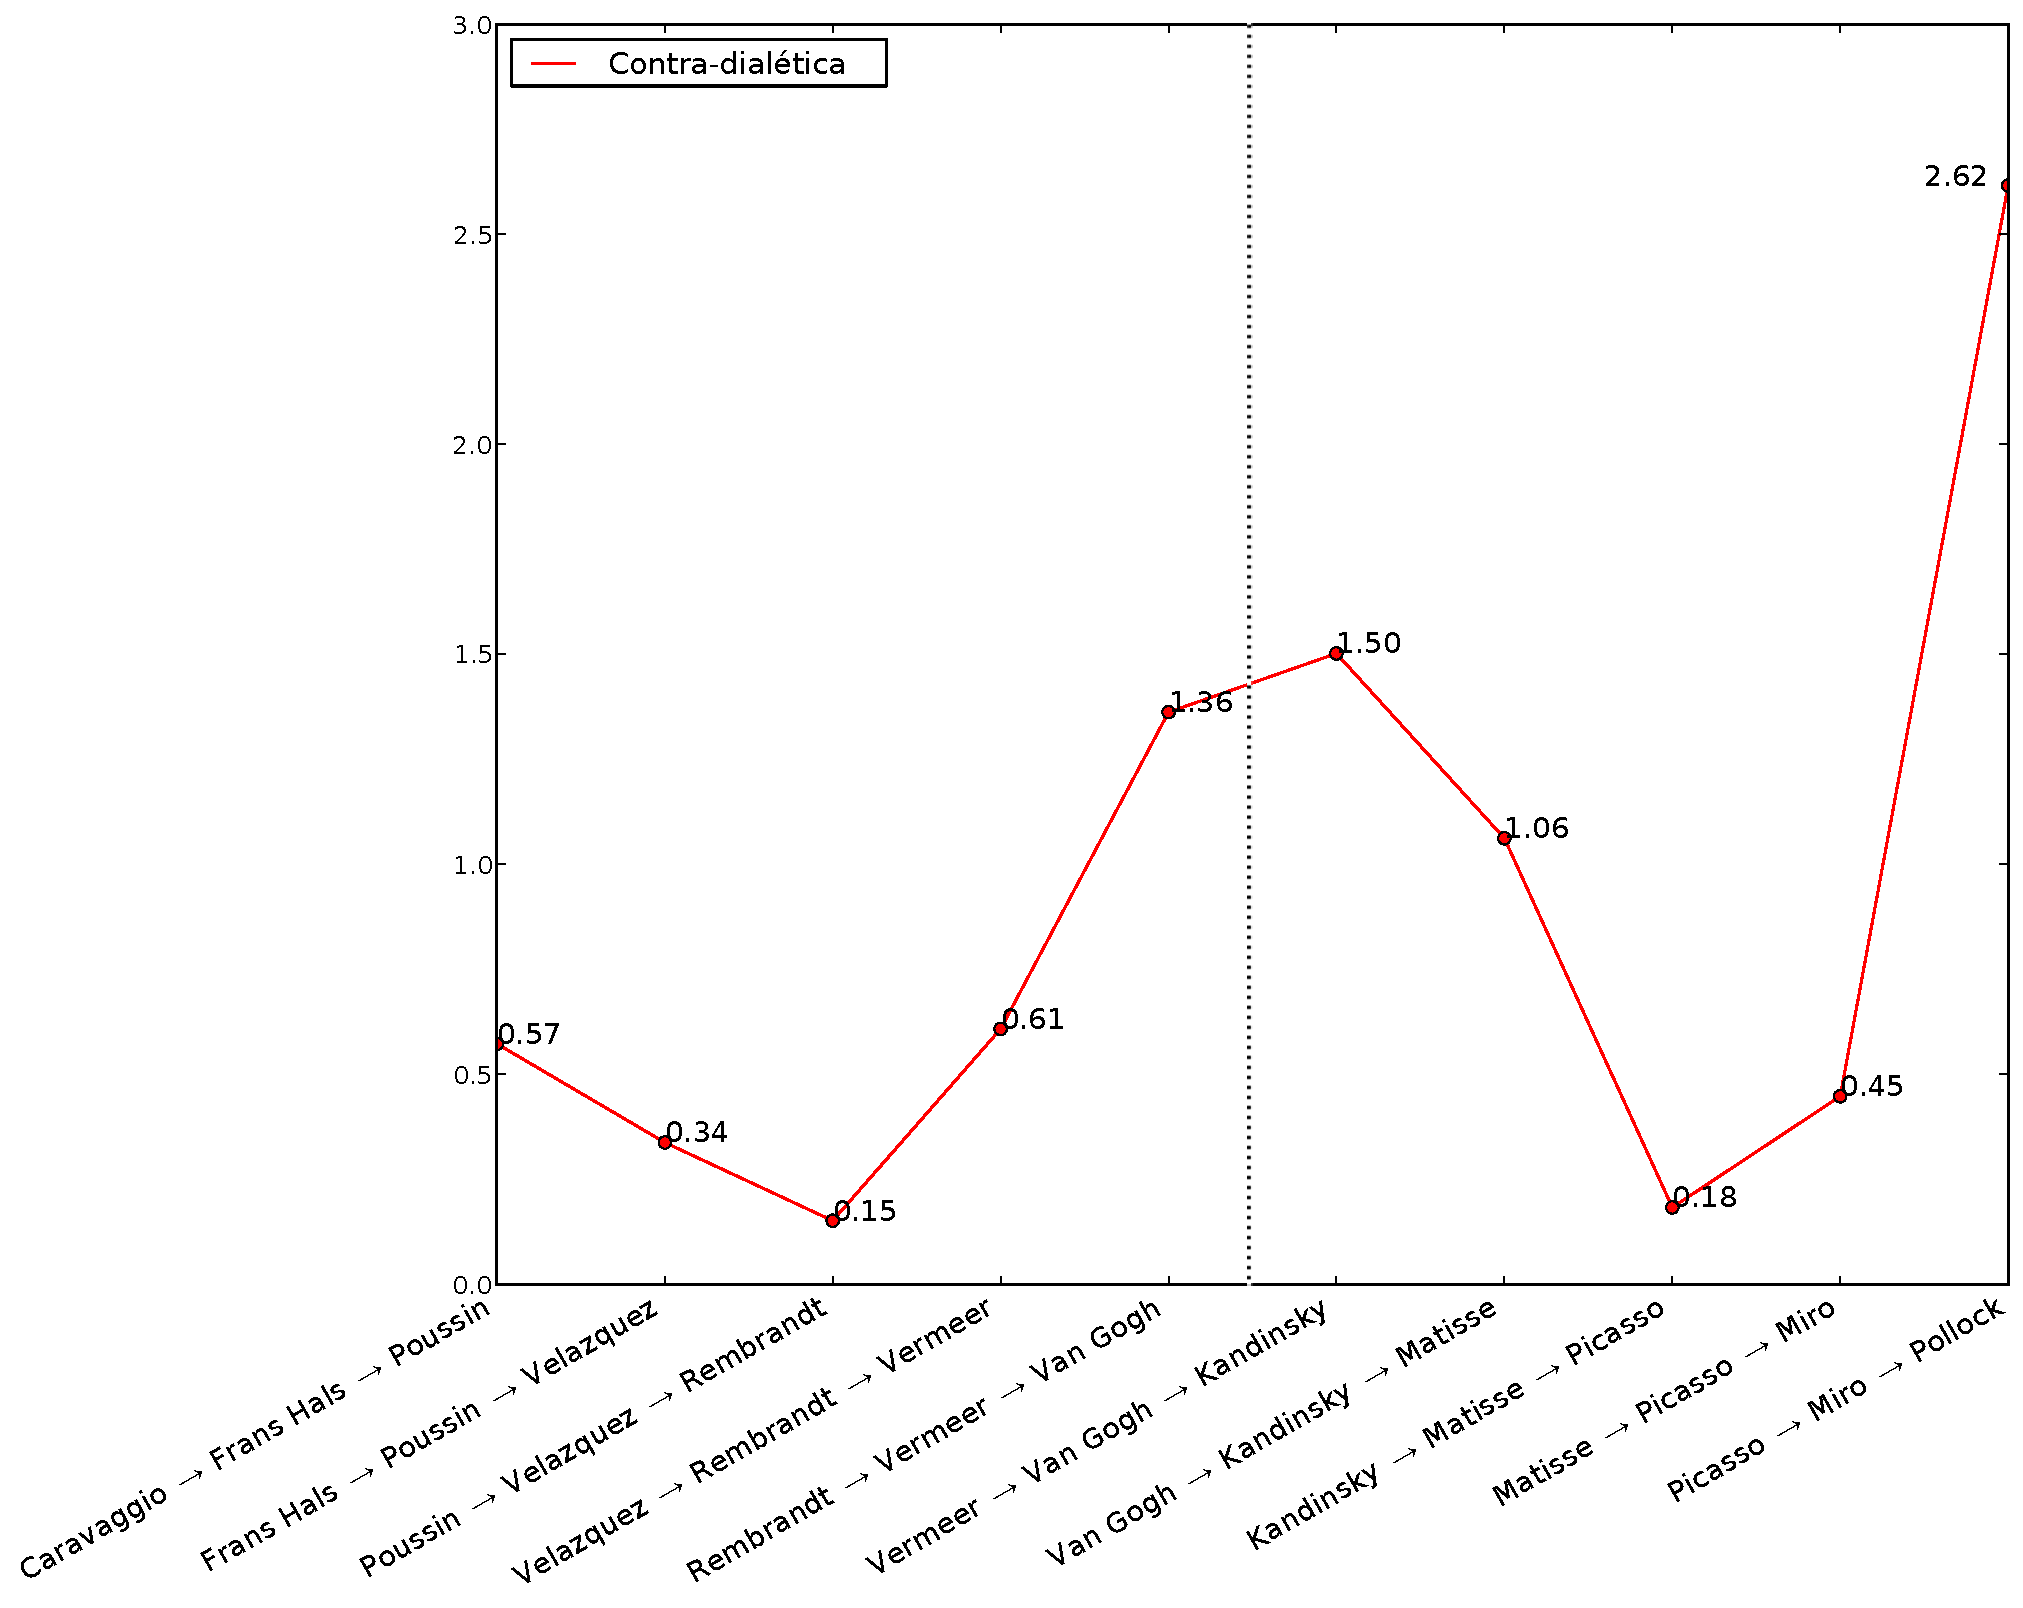
\includegraphics[width=.7\textwidth]{figs/caso1_dialetica}
         \caption{Valores de contra-dialética considerando os dois melhores atributos.}
        \label{fig:caso1_dialetica}
\end{center}
\end{figure}
\end{frame}

\begin{frame}{Dialética}
\setstretch{1.5}
      \begin{itemize}

  \item<1> Grande contra-dialética em Van Gogh.
  \item<1> $\to$ Início modernismo

  \item<2> Grande contra-dialética entre Caravaggio, Frans Hals e Poussin.
  \item<2> $\to$ Poussin realmente não representa a síntese entre Caravaggio e Frans Hals.

  \item<3> Maior dialética da série está em Poussin, Velázquez e Rembrandt.
  \item<3> $\to$ Rembrandt parece ser síntese entre Poussin (paisagens) e Velázquez (\textit{chiaroscuro}).

    \end{itemize}
\end{frame}

% \begin{frame}{Dialética}

%   \begin{columns}
%     \begin{column}{.49\textwidth}
%       \begin{itemize}

%   \item Kandinsky, por ser abstrato, diferencia-se de Vermeer e Van Gogh, apresentando a maior contra-dialética da série temporal.

%   \item Picasso possui grande dialética entre Kandinsky e Matisse.
%   %: suas pinturas retratam tanto elementos abstratos (Kandinsky) quanto figuras humanas (Matisse)

%   \item Pollock novamente apresenta o maior valor de contra-dialética.
%   %, distanciando-se de todos os demais artistas

%     \end{itemize}
%   \end{column}

%   \begin{column}{.49\textwidth}
%  \begin{figure}[h!]
% \begin{center}
%    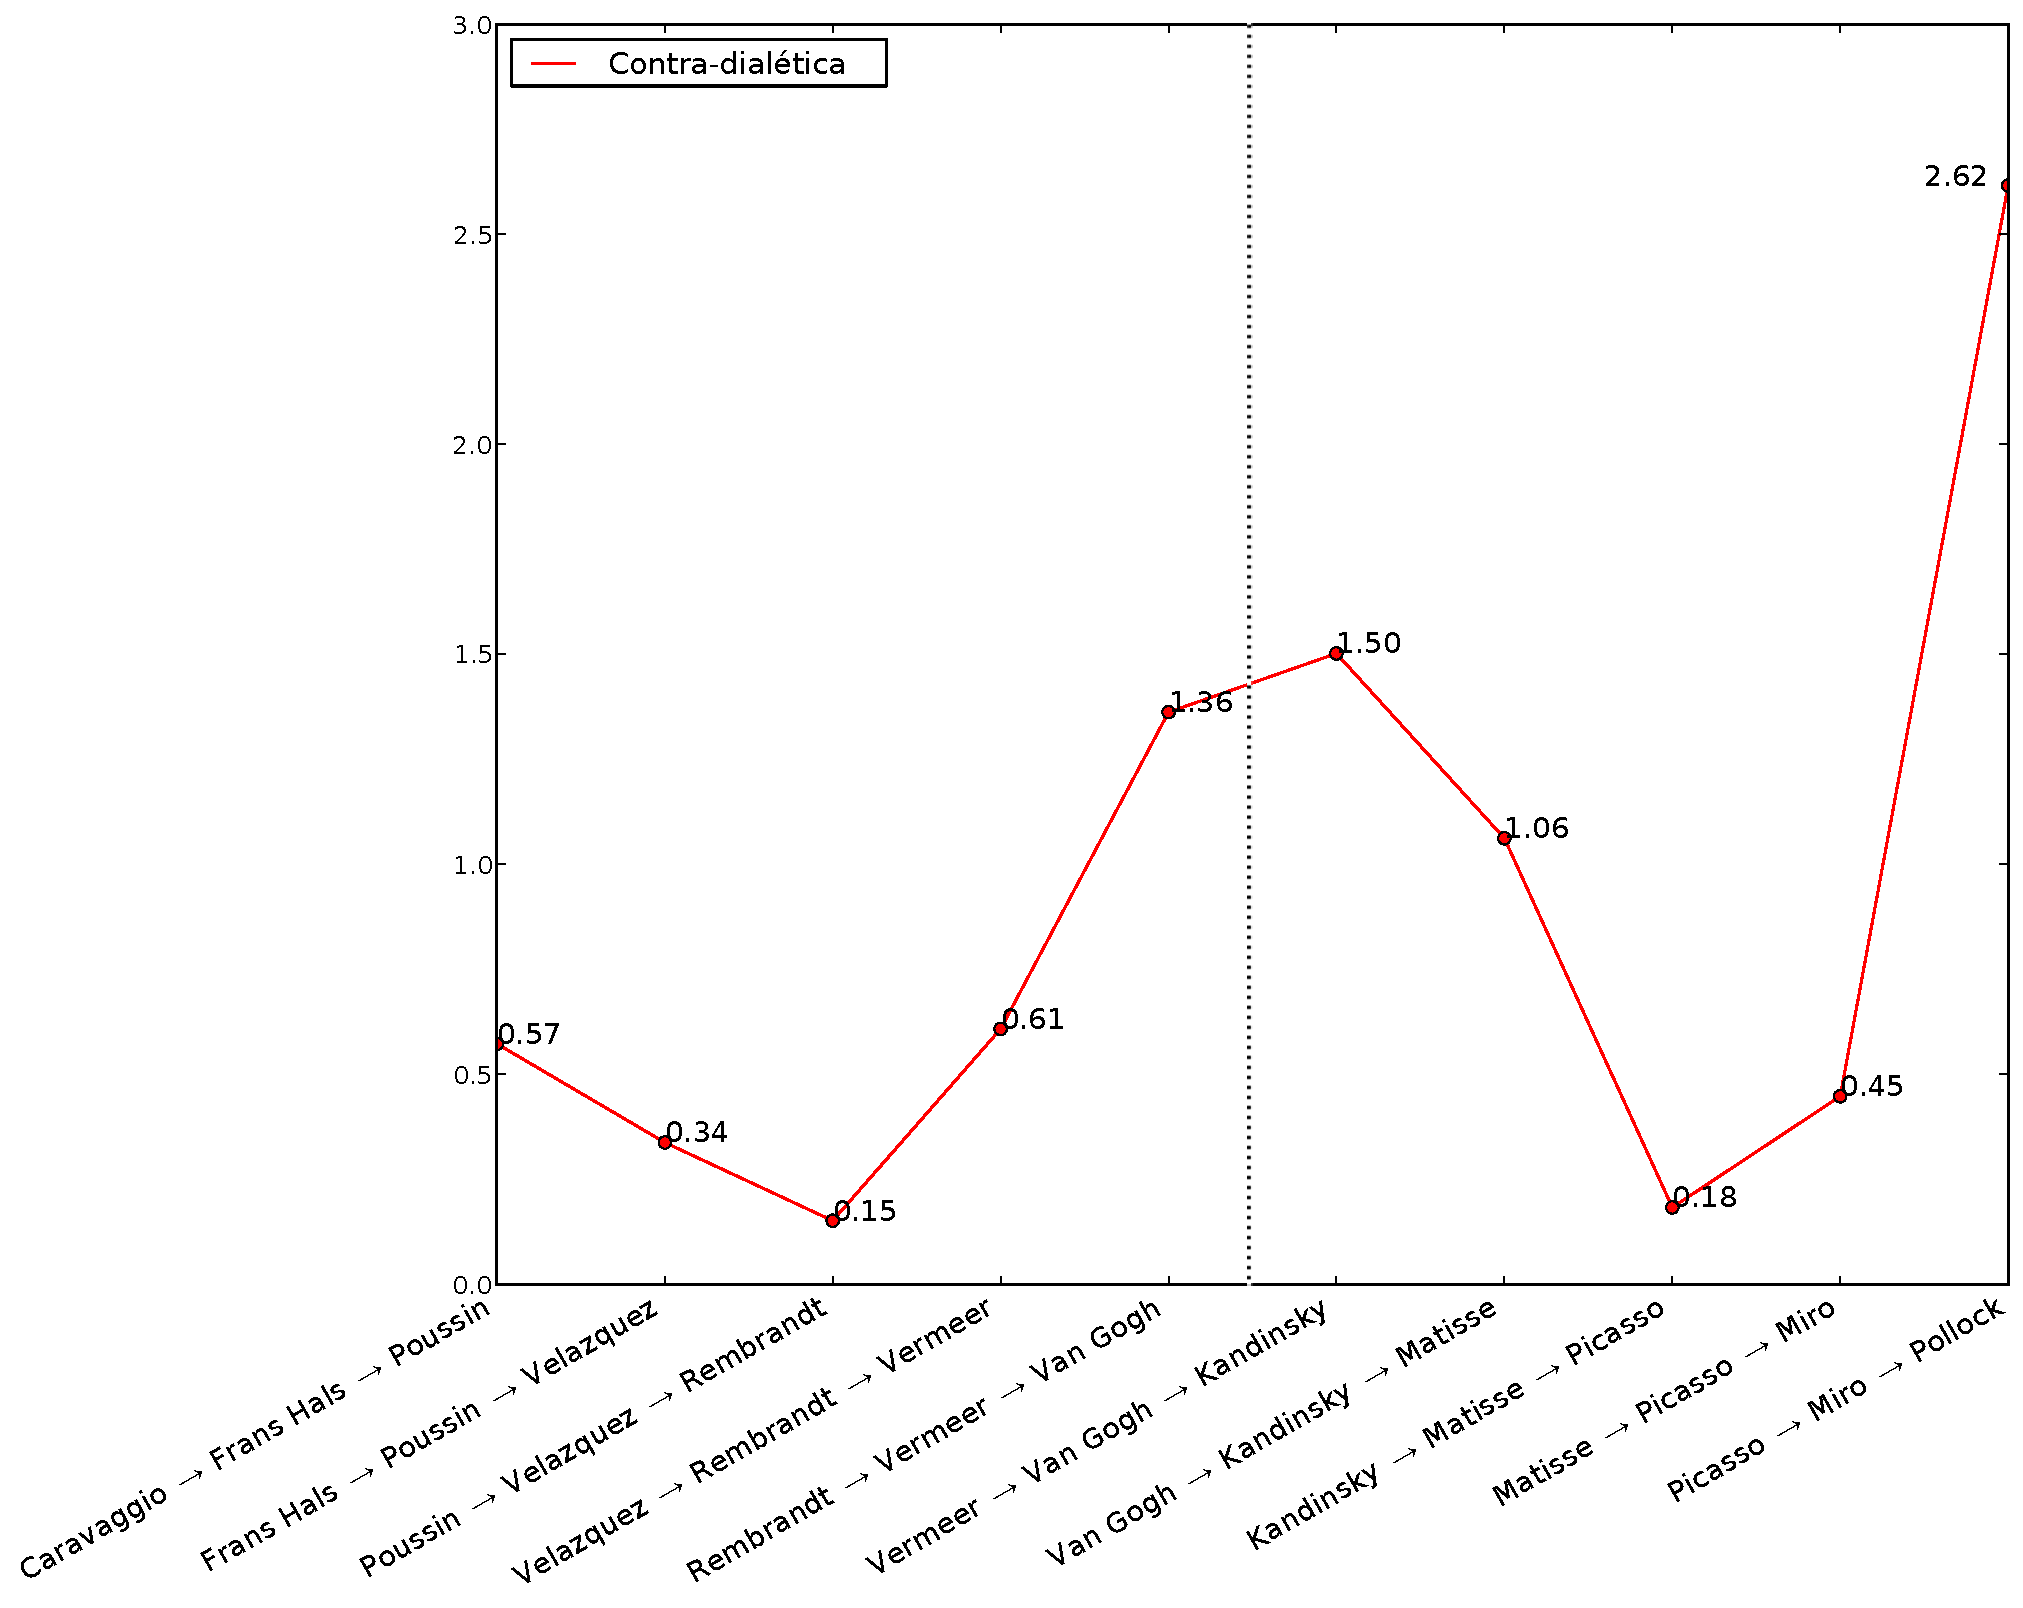
\includegraphics[width=\columnwidth]{figs/caso1_dialetica}
%        % \caption{Valores de contra-dialética considerando os dois melhores atributos.}
%        %  \label{fig:caso1_dialetica}
% \end{center}
% \end{figure}
%   \end{column}
% \end{columns}

% \end{frame}

% resultados => resultados para LDA

\begin{frame}{Resultados para LDA: projeções}

  \begin{columns}

   \begin{column}{.49\textwidth}
\begin{figure}[h!]
\begin{center}
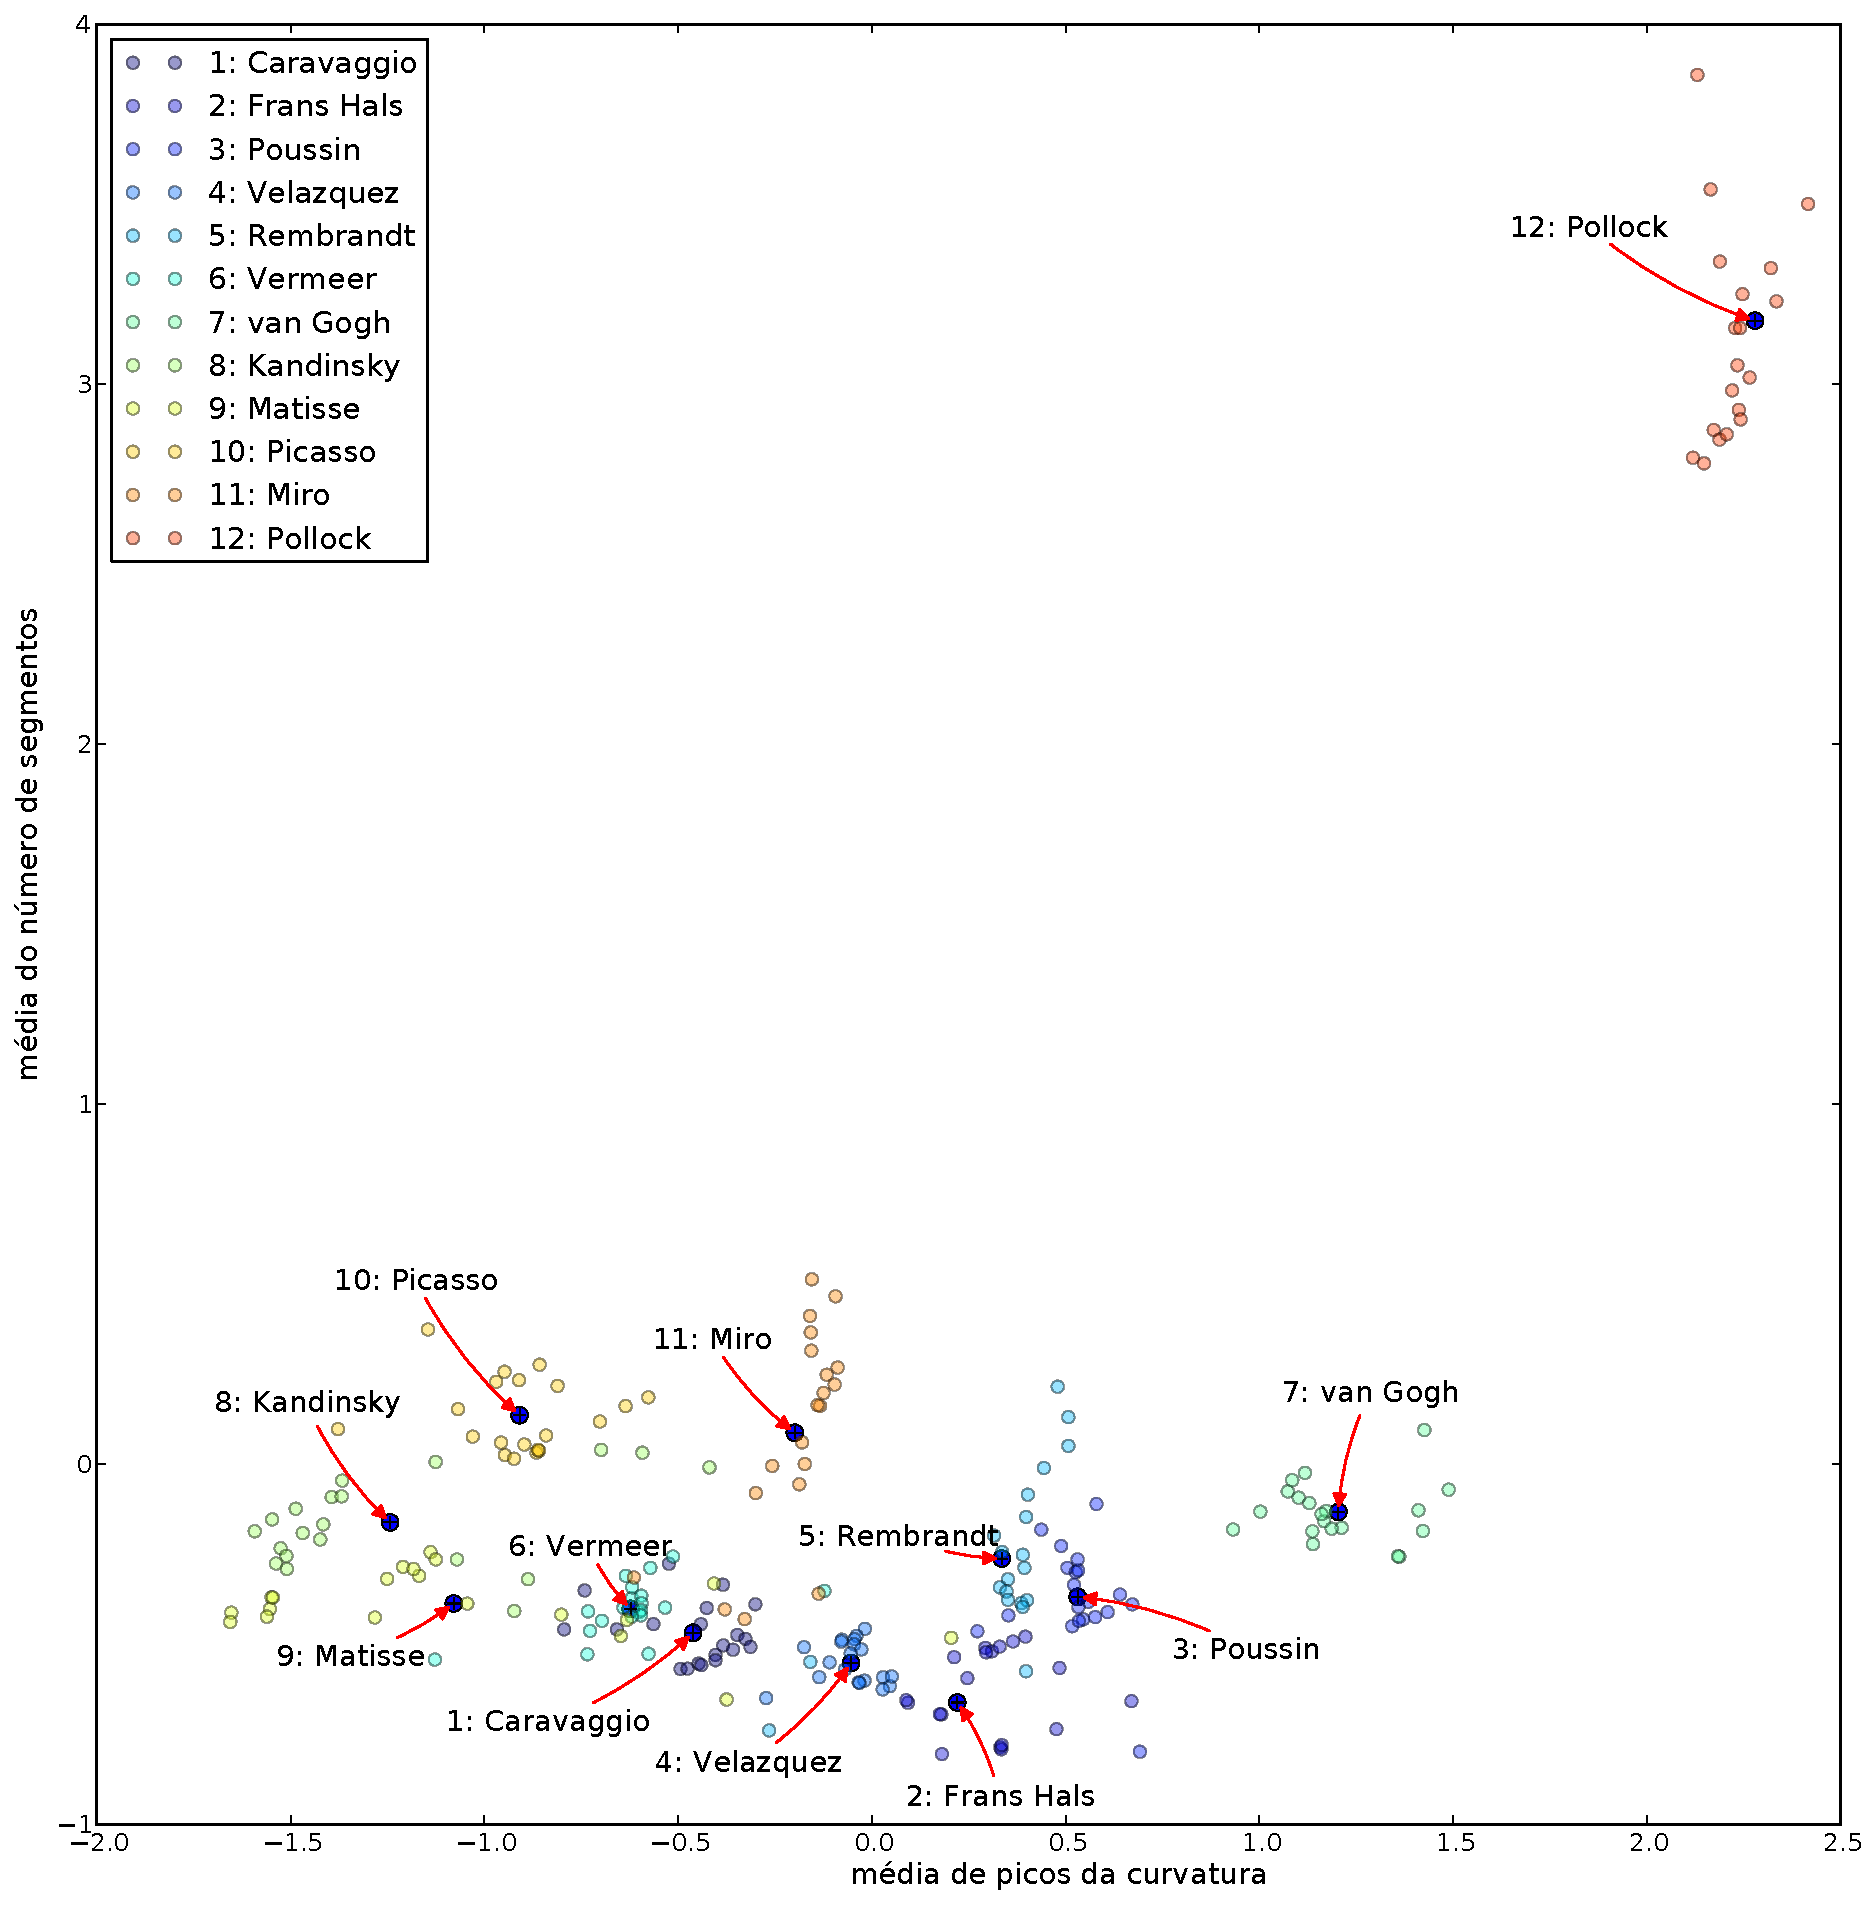
\includegraphics[width=\columnwidth]{figs/caso1_g1}
        \caption{Melhores atributos.}
\end{center}
\end{figure}
\end{column}


    \begin{column}{.49\textwidth}
\begin{figure}[h!]
\begin{center}
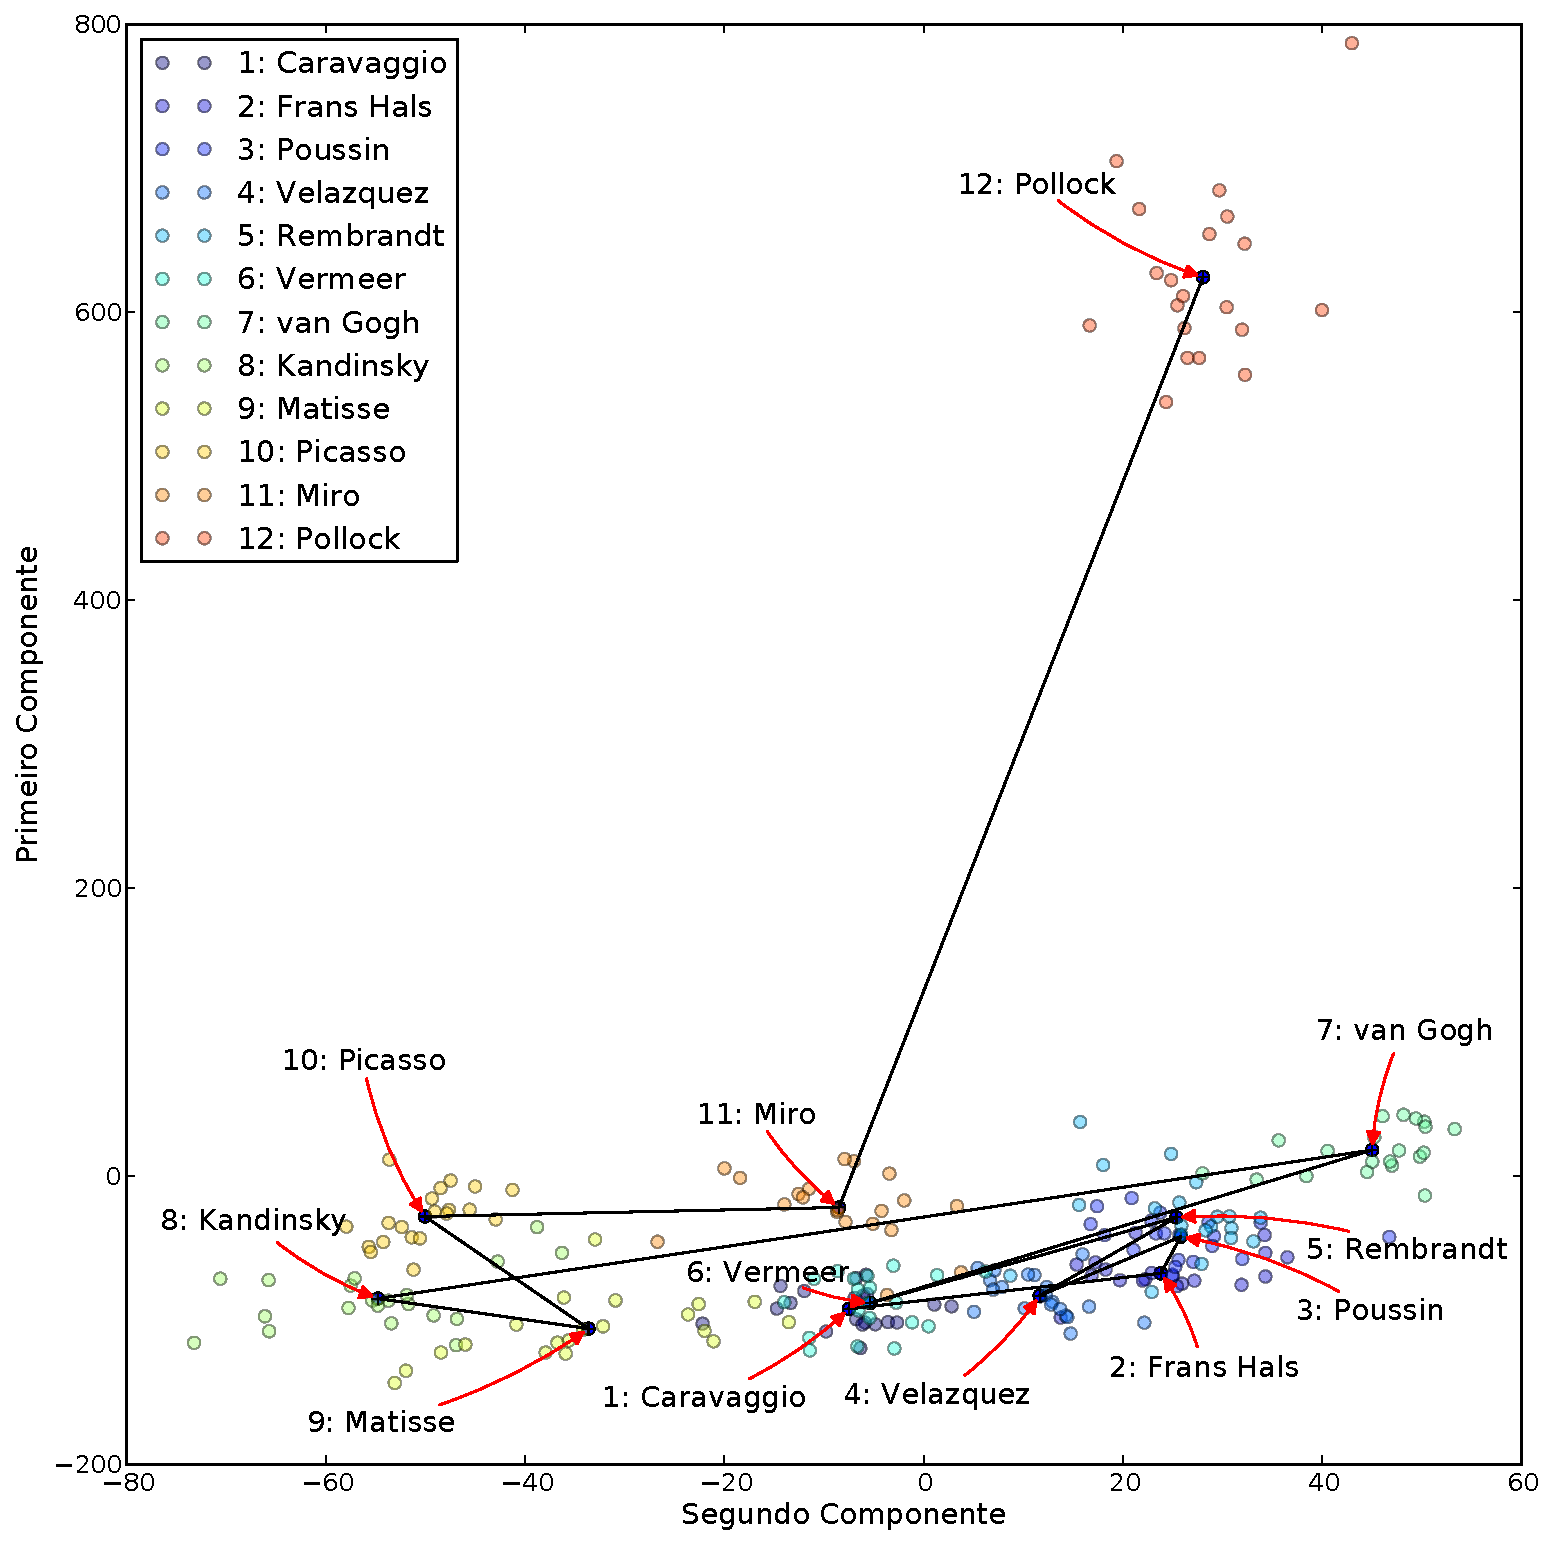
\includegraphics[width=\columnwidth]{figs/caso3_g1}
        \caption{LDA.}
\end{center}
\end{figure}
\end{column}
\end{columns}

\end{frame}

\begin{frame}{Resultados para LDA: oposição e inovação}

  \begin{columns}

   \begin{column}{.49\textwidth}
\begin{figure}[h!]
\begin{center}
\includegraphics[width=\columnwidth]{figs/caso1_oposEinov}
        \caption{Melhores atributos.}
\end{center}
\end{figure}
\end{column}


    \begin{column}{.49\textwidth}
\begin{figure}[h!]
\begin{center}
\includegraphics[width=\columnwidth]{figs/caso3_oposEinov}
        \caption{LDA.}
\end{center}
\end{figure}
\end{column}
\end{columns}

\end{frame}

\begin{frame}{Resultados para LDA: dialética}

  \begin{columns}

   \begin{column}{.49\textwidth}
\begin{figure}[h!]
\begin{center}
\includegraphics[width=\columnwidth]{figs/caso1_dialetica}
        \caption{Melhores atributos.}
\end{center}
\end{figure}
\end{column}


    \begin{column}{.49\textwidth}
\begin{figure}[h!]
\begin{center}
\includegraphics[width=\columnwidth]{figs/caso3_dialetica}
        \caption{LDA.}
\end{center}
\end{figure}
\end{column}
\end{columns}

\end{frame}

% resultados => validação por sampling aleatório (ver nome)

\begin{frame}{Validação do método LDA}
\setstretch{1.5}
  \begin{itemize}
    \item \textit{Cross validation} por \textit{repeated random sub-sampling}.

    \item 240 pinturas divididas em conjuntos de treino e teste.

    \item Para cada pintor, 10 pinturas de treino e 10 pinturas de teste.

    \item Processo repetido 100 vezes.
  \end{itemize}
\end{frame}

\begin{frame}{Validação do método}
\begin{figure}[h!]
\begin{center}
\includegraphics[width=.6\textwidth]{figs/matriz_confusao} 
      \caption{Matriz de confusão média para o método LDA calculada
        durante 100 iterações.}  \label{fig:cm}
\end{center}
\end{figure}
\end{frame}

% conclusões

\section{Conclusões}

% NEGRITO, PAUSE, SETSTRETCH

\begin{frame}{Conclusões}
\setstretch{1.5}
\begin{itemize}
  \item<1> Método quantitativo revelou resultados que encontram \textbf{fundamento na História das Artes}.

  \item<2> Medidas de \textbf{oposição, inovação e dialética} apresentaram resultados relevantes para o estudo da evolução artística na Pintura.

  \item<3> \textbf{Música} parece guiada pela \textbf{dialética} e \textbf{Filosofia} pela \textbf{oposição}.

  \item<4> Pintura teve \textbf{valores crescentes de inovação}; \textbf{picos de oposição e contra-dialética} em momentos de transição na história.
\end{itemize}

\end{frame}

\begin{frame}{Conclusões}
\setstretch{1.5}
\begin{itemize}
  \item<1> Um dos fatos mais marcantes na Pintura foi a \textbf{sobreposição dos Barrocos} e a \textbf{independência em estilo dos Modernos}.

  \item<2> Maior cobertura do \textit{espaço criativo} pelos Modernos.

  \item<3> Atributos de análise de forma (\textbf{número médio de picos de curvatura} e de \textbf{segmentos por imagem}) apresentaram melhor separação de classes.

  \item<4> LDA reforçou os resultados obtidos.
\end{itemize}

\end{frame}

\begin{frame}{Publicações}

  \begin{columns}

   \begin{column}{.49\textwidth}
\begin{figure}[h!]
\begin{center}
\includegraphics[width=\columnwidth]{figs/pub1} 
      \caption{\textit{A quantitative approach to evolution of music and philosophy}. \textbf{Journal of Statistical Mechanics}. 2012.}
\end{center}
\end{figure}
\end{column}

\begin{column}{.49\textwidth}
\begin{figure}[h!]
\begin{center}
\includegraphics[width=\columnwidth]{figs/physicaa1} 
      \caption{\textit{A quantitative approach to painting styles}. \textbf{Physica A: Statistical Mechanics and its Applications}. (arXiv 2013)}
\end{center}
\end{figure}
\end{column}

\end{columns}

\end{frame}

\begin{frame}{Contribuições artísticas}

\only<1>{
\begin{figure}[h!]
\begin{center}
\includegraphics[width=.7\textwidth]{figs/posterA} 
      \caption{Imagens generativas por triangulação de Delaunay.}
\end{center}
\end{figure}
}

\only<2>{
\begin{figure}[h!]
\begin{center}
\includegraphics[width=.8\textwidth]{figs/quiosque1} 
      \caption{Publicação impressa em revista independente. \textit{Fonte: Quiosque}.}
\end{center}
\end{figure}  
}

\end{frame}

\begin{frame}{Trabalhos futuros}
\setstretch{1.5}
  \begin{itemize}
    \item<1> Número de pintores e pinturas pode ser expandido, incluindo novos períodos.

    \item<2> Pode-se focar em apenas um período, buscando especificidades do período.

    \item<3>{Um conjunto de pintores específico pode ser analisado.
    \begin{itemize}
      \item Rafael, Poussin, Reni e Carracci;
      \item Filhos de Frans Hals e ele próprio;
      \item Cézanne, Matisse e Picasso.
    \end{itemize}
    }

    \item<4> Aplicação do mesmo método para outras áreas (e.g.\ MPB, Cinema e Literatura).

    \item<5> Utilização do método para geração de pinturas.

  \end{itemize}

\end{frame}

\begin{frame}{Agradecimentos}
\setstretch{1.5}
  \begin{itemize}
    \item Orientador prof. Gonzalo Travieso e co-orientador prof. Luciano da Fontoura Costa.

    \item Familiares, amigos e minha Gabriela.

    \item LabMacambira.sf.net e meus irmãos Renato e Ricardo Fabbri.

    \item \includegraphics[scale=.3]{figs/logo_capes} (2011-2013).
  \end{itemize}

\end{frame}

 \nocite{*}

\section{Referências}

\begin{frame}[allowframebreaks]{Referências}

%\bibliographystyle{apacite}
\bibliographystyle{plainnat}
\bibliography{main}
\end{frame}

\end{document}
